%% Template for Master thesis
%% ===========================
%%
\documentclass  [
  paper    = a4,
  BCOR     = 10mm,
  twoside,
  fontsize = 12pt,
  fleqn,
  toc      = bibnumbered,
  toc      = listofnumbered,
  numbers  = noendperiod,
  headings = normal,
  listof   = leveldown,
  version  = 3.03
]                                       {scrreprt}

\usepackage     [T1]                    {fontenc}
\usepackage                             {color}
\usepackage     [english]               {babel}
\usepackage                             {natbib}
\usepackage                             {hyperref}
\usepackage{graphicx}
\usepackage{framed}

\usepackage{amsmath}
\usepackage{amsfonts}
\usepackage[utf8]{inputenc}
\usepackage{hyperref}
\usepackage{cleveref}

\usepackage{algorithm}
\usepackage{algpseudocode}
%\usepackage{algcompatible}
%\usepackage{algorithm2e}

\usepackage{appendix}

\usepackage{float}


\newcommand\listappendixname{List of Appendices}
\makeatletter
\newcommand\listofappendices{%
	\chapter*{\listappendixname}\@starttoc{app}
}


\usepackage{enumerate}
%\usepackage[utf8]{inputenc}
\usepackage[top=1 in,bottom=1in, left=1 in, right=1 in]{geometry}
\usepackage[nottoc, notlof, notlot]{tocbibind}
%\usepackage{dsfont}

\newcommand{\matlab}{{\sc Matlab} }
\newcommand{\cvec}[1]{{\mathbf #1}}
\newcommand{\rvec}[1]{\vec{\mathbf #1}}
\newcommand{\ihat}{\hat{\textbf{\i}}}
\newcommand{\jhat}{\hat{\textbf{\j}}}
\newcommand{\khat}{\hat{\textbf{k}}}
\newcommand{\minor}{{\rm minor}}
\newcommand{\trace}{{\rm trace}}
\newcommand{\spn}{{\rm Span}}
\newcommand{\rem}{{\rm rem}}
\newcommand{\ran}{{\rm range}}
\newcommand{\range}{{\rm range}}
\newcommand{\mdiv}{{\rm div}}
\newcommand{\proj}{{\rm proj}}
\newcommand{\R}{\mathbb{R}}
\newcommand{\N}{\mathbb{N}}
\newcommand{\Q}{\mathbb{Q}}
\newcommand{\Z}{\mathbb{Z}}
\newcommand{\E}{\mathbb{E}}
\newcommand{\<}{\langle}
\renewcommand{\>}{\rangle}
\renewcommand{\emptyset}{\varnothing}

\newcommand{\mtrx}[1]{\begin{bmatrix}#1\end{bmatrix}}

\newtheorem{theorem}{Theorem}
\newtheorem{corollary}{Corollary}
\newtheorem{proposition}{Proposition}
\newtheorem{definition}{Definition}
\newtheorem{lemma}{Lemma}
\newtheorem{exercise}{Exercise}
\definecolor{darkblue}{rgb}{0.0,0.0,0.4}
\definecolor{darkgreen}{rgb}{0.0,0.4,0.0}
\hypersetup{
    colorlinks,
    linkcolor=black,
    citecolor=darkgreen,
    urlcolor=darkblue
}

\begin{document}
  %% title pages similar to providet template instead of maketitle
  %% This template was adjusted from the template of the department
%% for Physics and Astronomy for the master's program ``Scientific
%% Computing
%%
%% CC 2017 Michael Winckler
%%
%% More information:
%% http://www.physik.uni-heidelberg.de/aktuelles/studium/
%% (PDF link: ...studium/download/145/Vorlage_Diplomarbeit_Formular.pdf)

%% Titleintro
\thispagestyle{empty}
\begin{center}
  \renewcommand{\baselinestretch}{2.00}
  \Large\sffamily
  Department of Mathematics and Computer Science\\
  \large Heidelberg University
  \par\vfill\normalfont
  Master thesis\\
  in Scientific Computing\\
  submitted by\\
  Yu Xiang\\
  born in November 10, 1989\\
  2023
\end{center}
\newpage

%% Titlepage
\thispagestyle{empty}
\begin{center}
  \renewcommand{\baselinestretch}{2.00}
  \Large\bfseries\sffamily
    %Gradient method of solving parameterized optimal control problems, with a case study in state constrained rocket car %\\
    Numerical methods for optimal control problems, with a case study in state constrained rocket car %\\
    % (of)\\    
  \par
  \vfill
  \large\normalfont
  This master thesis has been carried out by Yu Xiang\\
  at the\\
  Heidelberg University \\
  under the supervision of\\
  Professor Dr. Ekaterina A. Kostina
  %% additionally insert second supervisor here if applicable
\end{center}\par
\vspace{5\baselineskip}

% reset baselinestretch
\renewcommand{\baselinestretch}{1.00}\normalsize 
   \tableofcontents
    \let\clearpage\relax
   \newpage
   % 

\chapter{Introduction}

Many real life problems, can be modeled as parameterized optimization problems, such as the therapy design of Cerebral Palsy (CP) problem described in \cite{MatSch22}. In this paper, we focus on using gradient method to solve parameterized optimization problems, with a case study in state constrained rocket car. 

Without giving a rigorous condition and definition\footnote{We do not give a rigorous definition on purpose so that the problem we have described here can be applied to more general cases when such condition and definition are more clearly defined.},  a general optimization problem is typically of the form
\begin{equation}
	\begin{aligned}
		 \  \  \ & min \  f(x) \\
		s.t.  \  \  \ & g(x) = 0, \\ 
		              &  h(x)  \geq  0 
	\end{aligned}
    \label{GeneralMin}
\end{equation}
where $f(x)$ is the objective or cost function, $g(x) = 0$ and $h(x)  \geq  0$ are the constraints. Some optimization problems may have uncertain parameters whose value are priori unknown, and the optimal objective value depends on the parameter value. This kind of problem is called the parameterized optimization problems and is of the form 


\begin{equation}
	\begin{aligned}
		\  \  \ & min \  f(x, p) \\
		s.t.  \  \  \ & g(x, p) = 0, \\ 
		&  h(x,p)  \geq  0  \\ 
		& x = x(p) \\
		& x = x(p^0) \  if \  p = p^0 \\
		& p \in \Omega_P		
	\end{aligned}
    \label{ParaMin}
\end{equation}
where $p^0$ is a fixed value in the feasible uncertainty set $\Omega_P$, where the parameter $p$ can take value from.

Parameterized optimization problems are very difficult to solve due to the uncertainty in the parameter $p$. In the paper \cite{MatSch22}, multiple methods of solving the parameterized optimization problem have been discussed. The main focus (of solving the Cerebral Palsy problem) of the paper \cite{MatSch22}, is the "worst-case treatment planning by bilevel optimal control", i.e. a bilevel optimization problem. The bilevel optimisation method in paper \cite{MatSch22} solves the parameterized optimization problems, e.g. the Cerebral Palsy problem, in a conservative way.


One method of solving the original CP problem in a conservative way is to transform the problem \ref{ParaMin} into another form. Assuming that the parameter $\tilde{p}$ lies in an uncertainty set $\Omega_P$, we can firstly reach one objective, i.e. identifying a worst possible solution with respect to $\tilde{p}$, i.e. solving a lower level problem. Based on the result of lower level, we can continue to find the best solution with respect to $x$, i.e. solving a upper level problem. The "worst-case treatment planning by bilevel optimal control", i.e. a  bilevel optimization problem, is an optimization problem in which another optimization problem enters the constraints. Mathematically, the problem \ref{ParaMin} is transformed into another form, and can be formulated in a simplified notation, as following


%\begin{equation}
%	\begin{aligned}
%		\  \  \ &  \underset{x}{min} \  \tilde f(x) \\
%		where  \  \  \ & \tilde f(x) =    \begin{cases}
%		  	\underset{p \in \Omega_P}{max} & \ f(x,p) \\
%			s.t.   & \  g(x, p) = 0, \  h(x,p)  \geq  0 \\
%		\end{cases}  	
%	\end{aligned}
%    \label{Bilevel}
%\end{equation}


%In a simplified notation, the problem can be written as 
\begin{equation}
	\begin{aligned}
		\underset{x}{min} \   \underset{p \in \Omega_P}{max} & \  f(x,p) \\ 
		s.t.  & \  g(x, p) = 0, \  h(x,p)  \geq  0 \\
	\end{aligned}
 \label{minmax}
\end{equation}


Due to the $min \ max$ notation, this classical approach of solving the bilevel problem can also be called $min max$ approach. 

As stated in \cite{MatSch22}, many different methods can be used to solve a bilevel problem, three approaches have been discussed in detail, i.e. a transformation of the bilevel problem to a single level problem, a classical approach and a training approach. A intuitive approach is to transfer the bilevel problem into a single level problem, however, in general the resulting single level problem is not equivalent to the original bilevel problem and this approach is also out of the focus of the paper \cite{MatSch22} as well as this paper at hand. A classical approach, aka a robust optimization appraoch, is consistent with the $minmax$ appoach, which will be discussed in more detail in Chapter 2.

The paper \cite{MatSch22} introduces the "Training Approach".  It is based on the idea that in the real world, during the training period, an intervention is introduced and a certain, but a priori unknown, parameter $p \in \Omega_P$ is realized. What follows the training period (during which the parameter $p$ is realized), the patient is able to react to it in an optimal manner, i.e. an optimal value $f(x,p)$ will be obtained given the  realized parameter $p$. The paper \cite{MatSch22} call this approach "worst case modeling Training Approach", and it can be written as 

\begin{equation}
	\begin{aligned}
		\underset{p \in \Omega_P}{max} \ \underset{x}{min} & \  f(x,p) \\ 
		s.t.  & \  g(x, p) = 0, \  h(x,p)  \geq  0 \\
	\end{aligned}
      \label{maxmin}
\end{equation}

Due to the $max \ mix$ notation, this approach of solving the bilevel problem can also be called $max min$ approach. 

The paper \cite{MatSch22} use a derivative free method in the Training Approach. This paper at hand will focus on a gradient method to solve the $maxmin$ problem.  In particular, we are interested in how to compute the derivatives theoretically and numerically.  We would like to apply the quasi-Newton and multiple shooting method when solving the problem numerically. The approaches discussed in this paper at hand will be demonstrated with a case study in state constrained rocket car. 

We choose this rocket car case for two reasons: firstly, the case is relatively easy to understand and is quite representative of the general usage in real life; secondly, the case has theoretical solution and we can compare the numerical results with the theoretical value so that we can check whether our gradient method can find the optimal solution and how fast it converges. 
 
The structure of this paper is as follows: in Chapter 1, i.e. this chapter,  we give an introduction on what problems this paper intends to address. In the Chapter 2, we introduce the case of the state constrained rocket car. In the Chapter 3, we discuss the classical approach and training approach, and show the theoretical value of the chosen case. In Chapter 4, we give the mathematical background of the quasi-Newton and multiple shooting method. In Chapter 5, we show how we can solve the case numerically using the methods described in Chapter 4. In Chapter 6, we compare our theoretical and numerical results and conclude the paper. 

\label{Chapter1}




\chapter{Rocket car case}
Since the approaches we are going to use in this paper will be demonstrated with the case of rocket car, we decide to describe the rocket car case first. So that, when we are discussing our approaches, we can directly describe how they can be used in solving the rocket car case. The description of the rocket car case is mostly coming from the paper \cite{MatSch22}, with content either verbatim or in a modified form. 

We consider the rocket car case with state constraints, i.e. the one-dimensional movement of a mass point under the influence of some constant acceleration/deceleration, e.g. modeling head-wind or sliding friction, which can accelerate and decelerate in order to reach a desired position. The mass of the car is normalized to 1 unit\footnote{We do not specify the unit on purpose since the actual unit, either one kilogram or meter, does not play a role in the modeling. We are more concerned about the scale.} and the constant acceleration/deceleration enters the model in form of an unknown parameter $p \in \Omega_P \subset \mathbb{R}$ suffering from uncertainty, with the uncertainty set $\Omega_P$ convex and compact. We consider a problem in which the rocket car shall reach a final feasible position and velocity in a minimum time: 



\begin{subequations}
	\begin{align}
	\underset{T, u(\cdot), x(:,p)}{min} \   & \  T \\ 
	s.t.  & \ \ x = (x_1, x_2)   \label{rc_x} \\ 
	& \ \  \dot{x} = T  \begin{pmatrix}  x_2(t;p) \\ u(t)-p   \end{pmatrix}, & \ t \in [0,1],  \label{rc_partial} \\
	& \ \ x(0,p) = 0, \label{rc_t0}\\
	& \ \ x_1(1;p) \geq 10, \label{rc_x1_t1} \\
	& \ \ x_2(t;p) \leq 4, & t \in [0,1], \label{rc_x2_tc} \\
	& \ \ x_2(1;p) \leq 0, \label{rc_x2_t1}  \\
	& \ \ T \geq 0, \\
	& \ \ u(t) \in [-10, 10], & t \in [0,1]. 
	\end{align}
	\label{rc}
\end{subequations}

where $x$ represents the variables of the rocket car, and it has two components $ x = (x_1, x_2)$. The first component $x_1$ is the (time-transformed) position of the rocket car. The second component $x_2$ is (time-transformed) velocity of the rocket car. The condition \ref{rc_t0}, i.e. $x(0,p) = 0$, indicates that at $t=0$, both the position and velocity of the car is $0$. The condition \ref{rc_x1_t1}, i.e. $x_1(1;p) \geq 10$, indicates that the position of the car at $t=1$ must be greater or equal to $10$. The condition \ref{rc_x2_t1}, i.e. $x_2(t;p) \leq 4$, indicates that the velocity of the car is always smaller or equal to 4 across the whole period. The condition \ref{rc_x2_t1}, i.e. $x_2(1;p) \leq 0$, indicates that the velocity of the car at $t=1$ is always smaller or equal to $0$. Here, a negative velocity means that the car is moving in a direction that decreases the position. To make the rocket car case even simpler, we can limit the size of the uncertainty set, as following
\begin{equation}
p \in \Omega_P = [p_l, p_u] \subset [0,9],
\end{equation}
where $p_l < p_u$, with $p_l$ and $p_u$ the lower and upper boundary of the parameter $p$.  

The decision variable in the problem \ref{rc} is the controllable parameter T, which encodes the process duration of the corresponding problem with free end time. The control function $ u: [0,1] \rightarrow \mathbb{R}$ represents the acceleration/deceleration value, and is dependent on the unknown parameter $p$, as shown in the condition \ref{rc_partial}. The second component of the condition \ref{rc_partial}, i.e. $\dot{x_2} = T (u(t)-p)$, indicates the change in the velocity of the car at time $t$ is subject to the value of $T, u(t)$ and $p$. The first component of the condition \ref{rc_partial}, i.e. $\dot{x_1} = Tx_2(t;p)$, indicates the position of the car at time $t$ is subject to the value of $T$ and the velocity $x_2(t;p)$ at time $t$. The variable $x(t:p)$ is a dependent variable, and is uniquely determined by $T, u(\cdot)$ and $p$. The goal is to minimize $T$ such that the variable $x(t:p)$ satisfies all the conditions in \ref{rc}. 

\section{Theoretical solution to rocket car case}
As explained in Chapter \ref{Chapter1}, we choose the rocket car case for two main reasons, i.e. the easyness of understanding and the existence of theoretical solution, which will be shown in this section. 



%There are three optimization variables in the optimization problem \ref{rc}, i.e. $T, u$ and $x$, and they belong to the following normed space
%\begin{equation}
%	(T, u(\cdot), x(:,p)) \in \mathbb{R} \times \mathbb{L}^\infty([0,1], \mathbb{R}) \times  \mathbb{W}^{1,\infty}([0,1], \mathbb{R}^2)
%\end{equation}
The optimization problem \ref{rc} has a unique global solution, and no further local solution exists. The optimal controllable parameter is given by 
\begin{equation}
T^\star = T^\star(p) = 2.5 + \frac{40}{100-p^2},
\end{equation}
and the optimal control function $u^\star(\cdot) (= u^\star(\cdot; p))$ by 
\begin{equation}
u^\star(\cdot) =     \left\{
\begin{array}{ll}
10, & for \  0 \leq t <  \frac{4}{(10-p)T^\star}\\
p  &  for \ \frac{4}{(10-p)T^\star} \leq t < 1- \frac{4}{(10+p)T^\star} \\
-10  & for \  1- \frac{4}{(10+p)T^\star} \leq t \leq 1 
\end{array}
\right.
\end{equation}

In words, we accelerate as strongly as possible (the acceleration value $u^\star(t)=10$) until the velocity $x^\star_2(t;p)=4$, and then keep the velocity $x^\star_2(t;p)$ constant for a certain periofd of time\footnote{The acceleration value cancels out with a inherent deceleration value so that the velocity can stay constant. The inherent deceleration value can be result of a friction or head wind.}, and eventually decelerate as as strongly as possible until the velocity is $x_2(1;p) \leq 0, \label{rc_x2_t1}$. The moment $x_2(1;p)$ reaching the value of $0$ is the moment that we finds the optimal/smallest $T$ that all the conditions are satisfied. 

The proof of the theoretical solution is given in Appendix B of \cite{MatSch22}. Because of the simplicity nature of the rocket car case, we can find the theoretical solution of the nominal/original problem for our case \ref{rc}. But for many real life problems, it is very difficult to find a direct solution to the original problem, and for some cases not feasible, due to the uncertainty in the parameter $p$. That is why in the paper \cite{MatSch22}, a classical (in the form $minmax$) approach and a training (in the form $maxmin$) approach have been discussed, and both approaches will lead to a conservative solution to the original problem. A conservative solution to the CP problem is a acceptable (or desired) result since less risk should be taken regarding the therapy design of CP problem. In the next chapter, we discuss, in details, the classical approaches and training approach for the rocket car problem. After that, we focus on the quasi-Newton and multi shooting approach to the same problem.  





\chapter{The Classical and Training Approach}

The paper on hand focuses on using quasi-Newton and multi-shooting method for the Training Approach. In this chapter, we shortly introduce the Classical Approach first and then we discuss the Training Approach in greater detail. In the next chapter, we can introduce the quasi-Newton and multi-shooting method, and elaborate in detail how they can be used for the Training Approach. 



\section{The Classical Approach}

As stated in the introduction part, the classical approach is consistent with the $minmax$ approach, during which, two level optimization problems are solved. 

In the lower level, we solve an optimization problem ($max \  f(x,p)$) with respect to $p$, and in the upper level, we continue to find the best solution with respect to $x$, as shown in \ref{minmax}. In the case of the rocket car, the classical approach will be expressed in the following form

\begin{subequations}
	\begin{align}
	\underset{T, u(\cdot)}{min} \  \underset{ p \in \Omega_P, x(\cdot,p)}{max}  \ \   & \  T \\ 
	s.t.  & \ \ x = (x_1, x_2)   \label{ca_rc_x} \\ 
	& \ \  \dot{x} = T  \begin{pmatrix}  x_2(t;p) \\ u(t)-p   \end{pmatrix}, & \ t \in [0,1],  \label{ca_rc_partial} \\
	& \ \ x(0,p) = 0, \label{ca_rc_t0}\\
	& \ \ x_1(1;p) \geq 10, & \ for \ all \ p \in \Omega_P, \label{ca_rc_x1_t1} \\
	& \ \ x_2(t;p) \leq 4, & t \in [0,1], \ for \ all \ p \in \Omega_P,  \label{ca_rc_x2_tc} \\
	& \ \ x_2(1;p) \leq 0, & \ for \ all \ p \in \Omega_P, \label{ca_rc_x2_t1}  \\
	& \ \ T \geq 0, \\
	& \ \ u(t) \in [-10, 10], & t \in [0,1]. 
	\end{align}
	\label{ca_rc}
\end{subequations}

In the Classical Approach, the set of feasible controllable parameters and control functions are given by those $T$ and $u(\cdot)$, which yield feasible trajectories $x(\cdot, p)$ for all $p \in \Omega_P$. The value of the objective function in the lower level does not depend on $p$ and $x(\cdot, p)$. In other words, in this approach, the driver has no prior knowledge about the value of the parameter $p$ and gets no feedback during the process and has to set up the driving strategy in advance. 

\section{The Training Approach}
Contrast to the Classical Approach, in the Training Approach it is assumed that the driver of the rocket car is able to perform optmially for every $p$ because of a preceding training period. Thus the worst possible optimal performance is given by a solution of the problem
\begin{subequations}
	\begin{align}
	\underset{p \in \Omega_P, T, u(\cdot), x(\cdot,p)}{max}  \ 	\underset{}{min} \   & \  T \\ 
	s.t.  & \ \ x = (x_1, x_2)   \label{ta_rc_x} \\ 
	& \ \  \dot{x} = T  \begin{pmatrix}  x_2(t;p) \\ u(t)-p   \end{pmatrix}, & \ t \in [0,1],  \label{ta_rc_partial} \\
	& \ \ x(0,p) = 0, \label{ta_rc_t0}\\
	& \ \ x_1(1;p) \geq 10, \label{ta_rc_x1_t1} \\
	& \ \ x_2(t;p) \leq 4, & t \in [0,1], \label{ta_rc_x2_tc} \\
	& \ \ x_2(1;p) \leq 0, \label{ta_rc_x2_t1}  \\
	& \ \ T \geq 0, \\
	& \ \ u(t) \in [-10, 10], & t \in [0,1]. 
	\end{align}
	\label{TA_rc}
\end{subequations}

The solution of the Training Approach in paper \cite{MatSch22} is given by a gradient-free method, more precisely, a so-called model-based Derivative-Free Optimization (DFO) approach for box-constrained optimization problems is used. The BOBYQA algorithm is chosen for such approach to solve problems of the form
\begin{equation}
\begin{aligned}
\underset{x \in \mathcal{R}^n}{min} & \  F(x)  \\ 
s.t.  & \ a_i \leq x_i \leq b_i, i = 1, ..., n \\
\end{aligned}
\label{DFO_bc}
\end{equation}

The name BOBYQA is an acronym for "Bound Optimization BY Quadratic Approximation", and is used to solve lower level problem of \ref{TA_rc}. In the general DFO method, the objective function $F(\cdot)$ is considered a black box. For a given $p$, the parametric lower level OCP of the Training Approach \ref{TA_rc} is solved with a direct DFO approach and the resulting (finite dimensional) solution is viewed as dependent variable. Furthermore, the uncentainty set $\Omega_P$ is box-shaped, and hence the BOBYQA algorithm is applicable to the problem in the Training Approach. The BOBYQA algorithm has been introduced in details in the paper \cite{MicPow09}, and we reiterate the main idea in the text that follows.  

The method of BOBYQA is iterative, $k$ and $n$ being reserved for the iteration number and the number of variables, respectively. Further, $m$ is reserved for the number of interpolation conditions that are imposed on a quadratic approximation $Q_k(x) \xrightarrow{} F(x), \ x \in  \mathcal{R}^n$, with $m$ is a chosen constant  integer from the interval $[n+2, \frac{1}{2}(n+1)(n+2)]$. 

The approximation is available at the beginning of the $k$-th iteration, the interpolation equations have the form
\begin{equation}
Q_k(y_j)= F(y_j),\   j = 1, 2, ..., m.
\end{equation}
We let $x_k$ be the point in the set $\{y_j : j = 1, 2, ... , m\}$ that has the property
\begin{equation}
F(x_k)= min\ \{F(y_j), \  j = 1, 2, ..., m\}, 
\end{equation}
with any ties being broken by giving priority to an earlier evaluation of the least function value $F(x_k)$. A positive number $\Delta_k$, called the “trust region radius”, is also available at the beginning of the $k$-th iteration. If a termination condition\footnote{Typically, a termination condition is satified when the objective value can not be improved further after some iterations. for the termination condition of BOBYQA algorithm, please refer the paper \cite{MicPow09} for more details.} is satisfied, then the iteration stops. Otherwise, a step $d_k$ from $x_k$ is constructed such that $ \Vert d_k \Vert \leq \Delta_k $ holds, $x = x_k+d_k$ is within the bounds of equation \ref{DFO_bc}, and $x_k+d_k$ is not one of the interpolation points $y_j : j = 1, 2, ... , m$. Then the new function value $F(x_k+d_k)$ is calculated, and one of the interpolation points, $y_t$ say, is replaced by $x_k+d_k$, where $y_t$ is different from $x_k$. It follows that $x_{k+1}$ is defined by the formula
\begin{equation}
x_{k+1} =
\begin{cases}
x_k, & F(x_k+d_k) \geq F(x_k) \\
x_k+d_k  , & F(x_k+d_k) < F(x_k) 
\end{cases}
\end{equation}

Further, $\Delta_{k+1}$ and $Q_{k+1}$ are generated for the next iteration, $Q_{k+1}$ being subject to the constraints 
\begin{equation}
Q_{k+1}(\hat{y}_j)= F(\hat{y}_j), \  j = 1, 2, ..., m, 
\end{equation}
at the new interpolation points
\begin{equation}
\hat{y}_j =
\begin{cases}
y_j, & j \neq t, \\
x_k+d_k  , & j =t 
\end{cases},  \  j = 1, 2, ..., m.
\end{equation}

The operations of BOBYQA algorithm requires the user to provide an initial vector of variables $x_0 \in \mathcal{R}^n$, the initial trust region $\Delta_1$, and the number $m$ of interpolation conditions where $n+2 \leq m \leq \frac{1}{2}(n+1)(n+2)$. Two different ways have been proposed for constructing the step $d_k$ from $x_k$ and updating procedures from the $k$-th iteration to the $k+1$-th iteration in the paper \cite{MicPow09}, with both methods having utilized the "quadratic" nature of the approximation function $Q(\cdot)$.

The lower level OCP of the Training Approach \ref{TA_rc} can be solved with the BOBYQA algorithm for a given $p$, since the lower level problem can be re-written into the form of \ref{DFO_bc} and the constraints are box-shaped. With the BOBYQA algorithm computing local extrema, the upper level problem still needs to be solved globally. In our rocket car case, this is straight-forward, i.e. maximizing over all $p$. 

Nevertheless, the BOBYQA algorithm has limitations with several strong assumptions being made. Firstly, it has been assumed the uncertainty set is of moderate size and is box-shaped. Secondly, it has been assumed that there is only one local extrema, i.e. the lower level problem has only one solution for each $p \in \Omega_P$. In general, we cannot expect the second assumption to be valid. The BOBYQA algorithm is a gradient-free method with repect to the objective function $F(\cdot)$, it still utilizes the gradient of the approximation function $Q(\cdot)$ while updating the iteration. Therefore, this BOBYQA algorithm, or a general DFO approach, is still subject to the numerical errors and computational costs while calculating the gradients of the approximation function $Q(\cdot)$  and updating them in each iteration.  

The paper at hand, instead, is utilizing the gradient of the objective function $F(\cdot)$ directly, with some approximation applied as well. We have used the multiple shooting and quasi-Newton method for solving the lower level problem of the Training Approach \ref{TA_rc}. In the chapter that follows, we introduce the quasi-Newton and multiple shooting method. 


\chapter{quasi-Newton and Multiple Shooting Method}
In this chapter, we first introduce the classical Newton method used for solving optimization problems and then focus on the quasi-Newton and multiple shooting method. 

As stated in the introduction chapter \ref{Chapter1}, a general optimization problem is typically of the form 
\begin{equation}
\begin{aligned}
\  \  \ & min \  f(x) \\
s.t.\ \  & x \in \Omega
\end{aligned}
\label{OptGen}
\end{equation}
Here $x \in \Omega$ represents the constraints for which $x$ must satisfy, it may be in the form of $ g(x) = 0,  h(x)  \geq  0$ as in the problem \ref{GeneralMin}, i.e. the feasible set $\Omega = \underset{x}{arg} \ \{ g(x) = 0,  h(x)  \geq  0 \}$. Various methods exist for eliminating the constraints, therefore, we can solve the resulting problem with algorithms for unconstrained minimization. For the sake of simplicity, we focus on explaining the Newton and quasi-Newton method without constraints in this chapter. How the quasi-Newton can be expanded for problems with constraints, will be explained in the next chapter. 


\section{Newton method}
The problem \ref{OptGen} without constraints, i.e. $min \  f(x)$  can be solved via Newton's method, which attempts to solve this problem by constructing a sequence $\{x_k\}$ from an initial guess (starting point) $x_0$ that converges towards a minimizer $x^\star$ of $f(x)$  by using a sequence of second-order Taylor approximations of $f(x)$ around the iterates. The second-order Taylor expansion of $f(x)$ around $x_k$ is
%\begin{multline*}
\begin{align*}
f(x_k + \delta_x) \approx h(x_k) : = f(x_k) + f'(x_k)\delta(x_k) +\frac{1}{2}f''(x_k)\delta(x_k)^2 
\end{align*}
where $\delta$ represents a small change (with respect to $x$), and $f', f''$ are the first and second order derivatives of the original function $f(x)$, and are usually denoted as $\nabla f$ and the Hessian matrix $H$ of $f(x)$ respectively when $x$ is a vector of multiple variables. In the text that follows, we will use the symbol $\nabla f$ and $H$ directly, therefore, the Talyor expansion can be written as 
\begin{align*}
f(x_k + \delta_x) \approx h(x_k) : = f(x_k) + \nabla f(x_k)^T\delta(x_k) +\frac{1}{2}H(x_k)\delta(x_k)^2 
\end{align*}
The next iterate $x_{k+1}$ is defined so as to minimize this quadratic approximation $h(\cdot)$. The function $h(\cdot)$ is a quadratic function of $\delta(x)$, and is minimized by solving $\nabla h(\cdot) = 0$. The gradient of $h(\cdot)$ with respect to $\delta(x_k)$ at point $x_k$ is
\begin{align*}
\nabla h(x_k) = \nabla f(x_k) + H(x_k) \delta(x_k) 
\end{align*}
We are motivated to solve $\nabla h(x_k) =0$, which leads to solve a linear system
%\begin{align*}
\begin{equation}
\nabla f(x_k) + H(x_k) \delta(x_k) =0
\label{HessianEq}
\end{equation}
%\end{align*}
Therefore, for the next iteration point $x_{k+1}$, we can just add the small change $\delta(x_k)$ to the current iterate, i.e. 
\begin{align*}
x_{k+1}  = x_k + \delta(x_k) = x_k - H^{-1}(x_k)\nabla f(x_k), 
\end{align*}
here $ H^{-1}(\cdot)$ represents the inverse of the Hessian matrix $H(\cdot)$. The Newton's method performs the iteration until the convergence, i.e. $x_k$ and $f(x_k)$ converge to $x^\star$ and $f(x^\star)$, respectively \footnote{In another word, the Newton mehtod has converged when the small change $\delta(x_k) =0$ or $\delta(x_k)$ is small enough that the change in the objective function is below a pre-defined tolerance level.}. The details of the Newton method is as follows: 
\begin{description}
	\item[Newton method steps]\ 
	\begin{itemize}
		\item Step 0, $k=0$, choose an initial value $x_0$ 
		\item Step 1, $\delta(x_k)  =- H^{-1}(x_k)\nabla f(x_k)$, if $\delta(x_k) =0$, then stop
		\item Step 2, choose a step-size $\alpha_k$ (typically $\alpha_k =1$)
		\item Step 3, set $x_{k+1}  = x_k + \alpha_k \delta(x_k) $, let $k= k+1$. Go to Step 1
	\end{itemize}
\end{description}

The parameter $\alpha_k$ is introduced to augment the Newton method such that a line-search of $f(x_k + \alpha_k \delta(x_k))$ is applied to find an optimal value of the step size parameter $\alpha_k$. 

Though the Newton method is straightforward and easy to understand, it has two main limitations. Firstly, it is sensitive to initial conditions. This is especially apparent if the objective function is non-convex. Depending on the choice of the starting point $x_0$, the Newton method may converge to a global minimum, a saddle point, a local minimum or may not converge at all. In another word, due to the sensitivity with respect to the initialization, the Newton method may be not able to find the global solution. Secondly, the Newton method can be computationally expensive, with the second-order derivatives, aka, the Hessian matrix $H(\cdot)$ and its inverse very expensive to compute. It may also happen that the Hessian matrix is not positive definite, therefore, Newton method can not be used at all for solving the optimization problem. Due to these limitations of the Newton method, we have chosen the quasi-Netwon method instead for solving our problem in the rocket car case. 

\section{quasi-Newton method}
We have stated that one limitation or the downside of the Newton method, is that Newton method can be computationally expensive when calculating the Hessian (i.e. second-order derivatives)  matrix and its inverse, especially when the dimensions get large. The quasi-Newton methods are a class of optimization methods that attempt to address this issue. More specifically, any modification of the Newton methods employing an approximation matrix $B$ to the original Hessian matrix $H$, can be classified into a quasi-Newton method. 

The first quasi-Newton algorithm, i.e. the Davidon–Fletcher–Powell (DFP) method, was proposed by William C. Davidon in 1959 \cite{WilDav59}, which was later popularized by Fletcher and Powell in 1963 \cite{FlePow63}. Some of the most common used quasi-Newton algorithms currently are the symmetric rank-one (SR1) method \cite{ANP91} and Broyden–Fletcher–Goldfarb–Shanno(BFGS) method. The family of the quasi-Newton algorithms are similar in nature, with most of the difference arising in the part how the approximation Hessian matrix is decided and the updating distance $\delta(x_k) $ is calculated. One of the chief advantages of the quasi-Newton methods over Newton's method is that the approximation Hessian matrix $B$ can be chosen in a way that no matrix needs to be directly inverted. The Hessian approximation $B$ is chosen to satisfy the equation \ref{HessianEq}, with the approximation matrix $B$ replacing the original Hessian matrix $H$, i.e. 
\begin{equation}
\nabla f(x_k) +B_k\delta(x_k) =0
\label{HessianAppro}
\end{equation}

In the text that follows, we explain how the iteration is performed in the BFGS method, as an example illustrating the quasi-Newton method. In the BFGS method, instead of computing $B_k$ afresh at every iteration, it has been proposed to update it in a simple manner to account for the curvature measured during the most recent step. To determine an update scheme for $B$, we will need to impose additional constraints. One such constraint is the symmetry and positive-definiteness of $B$, which is to be preserved in each update for $k = 1,2, 3, ...$. Another desirable property we want is for $B_{k+1}$ to be sufficiently close to $B_k$ at each update $k+1$, and such closeness can be measured by the matrix norm, i.e. the quantity $\Vert B_{k+1} - B_{k} \Vert$. We can, therefore, formulate our problem during the $k+1$ update as 
\begin{equation}
\begin{aligned}
\underset{B_{k+1}}{min} \  &  \Vert B_{k+1} - B_{k} \Vert\\
s.t.\ \  & B_{k+1}= B_{k+1}^T, \ B_{k+1}\delta(x_k)  = y_k \\
\end{aligned}
\label{BFGSB}
\end{equation}
where $\delta(x_k) = x_{k+1} -x_k$ and $y_k = \nabla f(x_{k+1}) - \nabla f(x_k)$. In the BFGS method, the norm is chosen to be the Frobenius norm:
\begin{align*}
\Vert B \Vert_F = \sqrt{\sum_{i}^{m} \sum_{j}^{n} |b_{ij}|^2} 
\end{align*}
Solving the problem \ref{BFGSB} directly is not trivial, but we can prove that problem ends up being equivalent to updating our approximate Hessian $B$ at each iteration by adding two symmetric, rank-one matrices $U$ and $V$:
%Solving the problem \ref{BFGSBUp} directly is not trivial, but we can prove that problem ends up being equivalent to updating our approximate Hessian $B$ at each iteration by adding two symmetric, rank-one matrices $U$ and $V$:
\begin{align*}
B_{k+1} = B_k + U_k + V_k
\end{align*}
where the update matrices can then be chosen to be of the form $U = a u u^T$ and $V = b v v^T$, where $u$ and $v$ are linearly independent non-zero vectors, and $a$ and $b$ are constants.  The outer product of any two non-zero vectors is always rank one, i.e. $U_k$ and $V_k$ are rank-one. Since $u$ and $v$ are linearly independent, the sum of $U_k$ and $V_k$ is rank-two, and an update of this form is known as a rank-two update. The rank-two condition guarantees the “closeness” of $B_k$ and $B_{k+1}$ at each iteration. 

Besides, the condition $B_{k+1}\delta(x_k) = y_k$ has to be imposed.
\begin{align*}
B_{k+1}\delta(x_k) = B_k\delta(x_k)  + a u u^T\delta(x_k) + b v v^T\delta(x_k) = y_k
\end{align*}

Then, a natural choice of $u$ and $v$ would be $u=y_k$ and $v=B_k\delta(x_k)$, we then have

\begin{align*}
B_k\delta(x_k) + a y_ky^T_k\delta(x_k) + bB_k\delta(x_k) \delta(x_k)^TB_k^T\delta(x_k) = y_k  \\
y_k(1-ay_k^T\delta(x_k) ) = B_k\delta(x_k)(1+ b \delta(x_k)^TB_k^T\delta(x_k)) \\
\Rightarrow a = \frac{1}{y_k^T\delta(x_k)}, \  b= - \frac{1}{\delta(x_k)^TB_k\delta(x_k)}
\end{align*}
Finally, we get the update formula as follows: 
\begin{align*}
B_{k+1} = B_k +  \frac{y_ky_k^T}{y_k^T\delta(x_k)}  - \frac{B_k\delta(x_k)\delta(x_k)^TB_k}{\delta(x_k)^TB_k\delta(x_k)}
\end{align*}

Since $B$ is positive definite for all $k = 1,2, 3, ...$, we can actually minimize the change in the inverse $B^{-1}$ at each iteration, subject to the (inverted) quasi-Newton condition and the requirement that it be symmetric. Applying the Woodbury formula , we can show (see the Appendix for more details) that the updating formula of inverse $B^{-1}$ is as follows

\begin{align*}
B_{k+1}^{-1} = (I - \frac{\delta(x_k)y_k^T}{y_k^T\delta(x_k)})B_k^{-1}(I - \frac{y_k\delta(x_k)^T}{y_k^T\delta(x_k)}) +  \frac{\delta(x_k)\delta(x_k)^T}{y_k^T\delta(x_k)} 
\end{align*}
As shown in the formula above, at each iteration, we update the value of $B^{-1}$ using only the values of $\delta(x_k) = x_{k+1} -x_k$ and $y_k = \nabla f(x_{k+1}) - \nabla f(x_k)$. Since an update of $B^{-1}$ depends on the previous value, we need to initialize $B^{-1}$, either as an identity matrix or as the true Hessian matrix $H(x_0)$, calculated based on the starting point $x_0$.

The problem \ref{TA_rc} involves constraints in the partial differential equation form. Therefore, we can apply multiple shooting method to transform the original problem into  discretized non-linear optimal control problem, with the constraints applied in each subinterval. Together with the matching conditions, we can then apply quasi  , apply multiple shooting and quasi-Newton method to get the optimal solution. In the text the follows, we explain the multilpe shooting method first and then focus on how it, together with quasi-Newton method, can be used for solving the rocket car problem.  

\section{Multiple Shooting Method}
Multiple shooting method was initially introduced to solve boundary value problem (BVP) in differential equation scope \cite{DJJ62}. This method, therefore, is well suited for solving optimal control problem which consists of differential equations with constraints. However, some modification is necessary so that the multiple shooting method can be applied to solve optimal control problem. In the text that follows, we first explain how the multiple shooting can be used for solving BVP in the differential equation scope. After that, we explain how mutilple shooting can be applied to a general optimal control problem, and particularly how it can be used for solving the rocket car case \ref{TA_rc}.

To illustrate the concept of shooting method to solve boundary value problem (BVP), we use the the following example.
\begin{align*}
\dot{x} = x(t), t_0 \leq t \leq t_f	
\end{align*}
The analytical solution of above equation is 
\begin{align*}
x(t) = x(t_0)e^{t - t_0}
\end{align*}
where $e$ is the exponential number. Then $x(t_0) = x_0$ will be determined such that it will satisfy
$x(t_f)=b$ for given value $b$. Therefore, the equation $x(t_f)-b = 0$ or $x_0e^{t - t_0}-b =0$ is obtained. This derivation is called as shooting method. Generally, the shooting method can be summarized as follow
\begin{description}
	\item[shooting method] \
	\begin{itemize}
		\item Step 1, choose an initial value $x_0 = x(t_0)$ 
		\item Step 2, form a solution of the differential equation from $t_0$ to $t_f$
		\item Step 3, evaluate an error of the boundary condition, if $x(t_f) - b = 0$, then stop, otherwise continue to Step 4 
		\item Step 4, update the guess for $x_0$ based on some updating schema, go to Step 2
	\end{itemize}
\end{description}

In multiple shooting method, the "shoot" interval is partitioned into some short intervals. We define a general differential equation with boundary value of the following form
\begin{equation}\label{eqn:ori_dae}
\begin{aligned}
& \dot{y} = f(t, y, p) \\ 
& y(t_f) = y_f  \\
\end{aligned}
\end{equation}
where $y$ denotes the differential variables, $p$ is some parameter, $t \in [t_0, t_f]$,  $y_f$ is the boundary value at $t_f$.  With multiple shooting method, one chooses a suitable grid of multiple shooting nodes $\tau_j \in [t_0,t_f] $, where $t_0 = \tau_0 < \tau_1 < ... < \tau_m = t_f$,  i.e. $m$ subintervals covering the whole interval. At the beginning of each subinterval, $[\tau_k, \tau_{k+1}], k = 0, 1, ..., m-1$, we have the initial guess of the starting value $\hat{y}_k$. Then in each subinterval, we have the initial value problem of the following form: 
\begin{equation}\label{eqn:msh}
\begin{aligned}
& \dot{y} = f(t, y, p) , t \in [\tau_k, \tau_{k+1}], \ k = 0, 1, ..., m-1   \\ 
& y(\tau_k) = \hat{y}_k, k = 0, 1, ..., m-1  \\
\end{aligned}
\end{equation}
In each subinterval, we introduce the new unkown parameter $\hat{y}_k$, we solve an initial value problem and will get a solution $y(t), t \in [\tau_k, \tau_{k+1}]$. The piecewise solution is not necessary continuous and also not necessarily satisfy the boundary condition $y(t_f) = y_f$. The continuity has to be enforced by additional matching conditions at each subinterval point, i.e. 
\begin{equation}\label{eqn:mc}
\begin{aligned}
& y(\tau_{k+1}; \hat{y}_k) = \hat{y}_{k+1}, \  k = 0, 1, ..., m-1  \\
& \hat{y}_{m} = \hat{y}_{\tau_m} = \hat{y}_{t_f} =  y_f 
\end{aligned}
\end{equation}

The procedure of multiple shooting method can then be summarized as
\begin{description}
	\item[Mutilple shooting method] \
	\begin{itemize}
		\item Step 1, choose multiple shooting nodes $t_0 = \tau_0 < \tau_1 < ... < \tau_m = t_f$ 
		\item Step 2, choose initial guess for $\hat{y}_k, k = 0, 1, ..., m-1$ 
		\item Step 3, form solutions of the differential equation in each subinterval $[\tau_k, \tau_{k+1}], k = 0, 1, ..., m-1$
		\item Step 4, evaluate the error at boundary of each interval condition, if $y(\tau_{k+1}; \hat{y}_k) - \hat{y}_{k+1} = 0, \  k = 0, 1, ..., m-1$ and $\hat{y}_{m} = y_f$, then stop, otherwise cotinue to Step 5
		\item Step 5, update the guess for $\hat{y}_k, k = 0, 1, ..., m-1$ based on some updating schema, go to Step 3
	\end{itemize}
\end{description}

In practice, there are many details to be decided when using (multiple) shooting methods, which we will introduce briefly without giving a rigorous formation. In Step 1 \& 2, when choosing the shooting nodes and the initial guess $\hat{y}_k$, how they are chosen usually depends on nature of the problem as well as a balance between accuracy and computational cost. For example, the nodes can be equally spaced and the $\hat{y}_k$ can be initialized with the same value, or they can be addressed in other methods. In Step 3, polynomial functions can be used as the approximate solutions, leveraging the fact that Taylor expansion can be used to approximate any continuous functions. In Step 4, "evaluate the error" is usually in the form of evaluating an objective function, which, e.g. can be defined as the sum of quadratic errors. In Step 5, the "updating schema" can be defined to so that the $\hat{y}_k$ can move in a direction that decreases the objective function. The (quasi) Newton method, for example, can be used as an updating method in Step 5. 


The multiple shooting method can be used for many problems. For example, it can be applied to the twice differential system of the following form 
\begin{equation*}
y''(t) = f(t, y(t), y'(t))  \quad y(t_0) = y_0, \quad y(t_f) = y_f,  \quad t \in [t_0, t_f]
\label{eqn:tdode}
\end{equation*}
The problem above is similar to the problem \ref{eqn:ori_dae}. In each subinterval, a boudary value problem (BVP) is to be solved and matching conditions at the boundary of each subinterval  are to be enforced applied so that the final solution found is applicable to the whole interval. 


With the same idea, we can use mutiple shooting to solve a optimal control problem. For the rocket car problem \ref{TA_rc}, we can discretize the time $t \in [0, 1]$ and the original OCP problem is split into multiple intervals, with the constraints also applied to each subinterval. We also need to introduce the initial guess for each interval and add the matching constraints. In the end, we turn the original problem  \ref{TA_rc} into piecewise OCPs with augmented parameters and constraints. But the piecewise OCPs can be solved as as a whole due to their non-overlapping properties and same structure, i.e. they can be aggregated to one objective function with the constraints expressed in matrix form. The final problem can then be solved with quasi-Newton method. In the next chatper, we discuss in detail how the problem \ref{TA_rc} can be solved with mutiple shooting method and quasi-Newton method in details. 


\chapter{Rocket Car Case}
Before we dive into the mathematics, we first re-introduce the physics of the rocket car case so that we can model the problem more precisely. Within the training approach, with a given $p$, we want to solve the lower level problem of the following form \ref{TA_lower}
\begin{subequations}
	\begin{align}
	\underset{}{min} \   & \  T \\ 
	s.t.  & \ \ x = (x_1, x_2)   \label{ta_rc_x} \\ 
	& \ \  \dot{x} = T  \begin{pmatrix}  x_2(t;p) \\ u(t)-p   \end{pmatrix}, & \ t \in [0,1],  \label{ta_rc_partial2} \\
	& \ \ x(0,p) = 0, \label{ta_rc_t2}\\
	& \ \ x_1(1;p) \geq 10, \label{ta_rc_x1_t2} \\
	& \ \ x_2(t;p) \leq 4, & t \in [0,1], \label{ta_rc_x2_tc2} \\
	& \ \ x_2(1;p) \leq 0, \label{ta_rc_x2_t1_2}  \\
	& \ \ T \geq 0, \\
	& \ \ u(t) \in [-10, 10], & t \in [0,1], \\
	& \ \ p, \   a \ given \ value
	\end{align}
	\label{TA_lower2}
\end{subequations}

In summary, we want to find the minimum time that the rocket car moves from the starting state (the position is at the origin point, and the speed is zero) to an ending state when the position is at least at point 10 or beyond, and the speed is less than or equal to zero (a negative speed indicates the car is moving in a direction that decreases the position), with constraints on the acceleration/deceleration value and the speed during the whole process. 

Because our objective is to minimize the time between starting state and ending state, i.e. the variable $T$, which is unknown, we cannot define a time horizon over which we will discretize and optimize. Therefore, a new variable $t$ is defined as follows: 
\begin{equation*}
t= \frac{\tau}{T} \in [0,1] \quad \tau \in [0, T]
\label{eqn:timet}
\end{equation*}

Where $\tau$ is the real time between starting time $0$ and ending time $T$, and $t$ is the relative time between $0$ and $1$.  The equation \ref{ta_rc_partial2} can be also written as 

\begin{subequations}
	\begin{align}
	\dot{x} =  \begin{pmatrix} \dot{x_1} \\ \dot{x_2} \end{pmatrix}  & =  T  \begin{pmatrix}  x_2(t;p) \\ u(t)-p   \end{pmatrix} = \begin{pmatrix}  Tx_2(t;p) \\ T(u(t)-p)   \end{pmatrix} \label{eq_difT} \\ 
	\begin{pmatrix} \dot{x_1} \\ \dot{x_2} \end{pmatrix} &= \begin{pmatrix} \frac{\partial x_1}{\partial t} \\ \frac{\partial x_2}{\partial t} \end{pmatrix} = \begin{pmatrix} \frac{\partial x_1}{\partial \tau} \frac{\partial \tau}{\partial t} \\ \frac{\partial x_2}{\partial \tau} \frac{\partial \tau}{\partial t} \end{pmatrix} =  \begin{pmatrix} \frac{\partial x_1}{\partial \tau} T \\ \frac{\partial x_2}{\partial \tau}T \end{pmatrix} =     \begin{pmatrix}  Tx_2(t;p) \\ T(u(t)-p)   \end{pmatrix} \\
	\begin{pmatrix} \frac{\partial x_1}{\partial \tau}  \\ \frac{\partial x_2}{\partial \tau} \end{pmatrix} & =     \begin{pmatrix}  x_2(t;p) \\ (u(t)-p)   \end{pmatrix} \label{eq_difTau}
	\end{align}
\end{subequations}

In summary, the equation $\frac{\partial x_1}{\partial \tau}= x_2(t;p) $ means the change in the position in real time is proportional to the speed at that moment. And the equation $\frac{\partial x_2}{\partial \tau} = u(t)-p $ means the change in speed is proportional to the acceleration/deceleration value at that moment. 

To use multiple shooting and quasi-Newton method, we discretize the interval $t\in [0,1]$ into subinterval $[t_{k-1}, t_k], k = 1, 2, ..., m$, where $0 =t_0, t_1, t_2, ...,t_{k-1}, t_k, ..., t_m=1$. We solve the OCP within each interval, and enforce the matching condition at the boundary of each interval. 

The equation \ref{eq_difT} is equivalent to \ref{eq_difTau}





% t&= \frac{\tau}{T} \in [0,1] \quad \tau \in [0, T]
%\\
%i.e. \ \begin{pmatrix} \dot{x_1} \\ \dot{x_2} \end{pmatrix} &= \begin{pmatrix} \frac{\partial x_1}{\partial t} \\ \frac{\partial x_2}{\partial t} \end{pmatrix} = 
%\begin{pmatrix} \frac{\partial x_1}{\partial \tau} \frac{\partial \tau}{\partial t}  \\ \frac{\partial x_2}{\partial \tau} \frac{\partial \tau}{\partial t} \end{pmatrix} 

%\begin{equation*}
%	\begin{align}
%		\dot{x} =  \begin{pmatrix} \dot{x_1} \\ \dot{x_2} \end{pmatrix}  & =  T  \begin{pmatrix}  x_2(t;p) \\ u(t)-p   \end{pmatrix} = \begin{pmatrix}  Tx_2(t;p) \\ T(u(t)-p)   \end{pmatrix} \\
%		i.e. \ \begin{pmatrix} \dot{x_1} \\ \dot{x_2} \end{pmatrix} &= \begin{pmatrix} \frac{\partial x_1}{\partial t} \\ \frac{\partial x_2}{\partial t} \end{pmatrix} = 
%		\begin{pmatrix} \frac{\partial x_1}{\partial \tau} \frac{\partial \tau}{\partial t}  \\ \frac{\partial x_2}{\partial \tau} \frac{\partial \tau}{\partial t} \end{pmatrix} 
%	\end{align}
%\end{equation*}







   
   
 \chapter{Introduction}  
 \label{Chapter1}
Many real-life problems can be modeled as an optimal control problem (OCP), for example, launching a rocket to the moon with minimum fuel expenditure as the objective, or maximizing the profit from factory production, with constraints on resources available and uncertain market demand. This paper focuses on solving optimal control problems with numerical approaches, particularly with multiple shooting and (quasi) Newton type methods. 

In general, optimal control deals with the problem of finding control over the state of a dynamic system over a period of time such that an objective function is optimized. Generally, an optimal control problem can be formulized as follows: 
      \begin{equation}
   	\begin{aligned}
   	\underset{x(\cdot), u(\cdot)}{\text{min}}  \ &  F(x(\cdot), u(\cdot)) \\
   		s.t.\ \  &  \dot{x} (t) = f(x(t), u(t))\\ 
   		        & x(t) \in \Omega \\
   		          & u(t) \in \mathbb{U}  \\
   		          & t \in [t_0, t_f]
   	\end{aligned}
   	\label{P1_OPH}
   \end{equation}
% Here $t$ is the independent variable (generally speaking, time), usually using $t_0$ and $t_f$ representing the initial and terminal time respectively. $x(t)$ is the state variables, and $u(t)$ is the control variables, $F(\cdot)$ is the objective function, also called the cost function. $\dot{x} (t) = f(x(t), u(t))$ represents the underlying dynamic system,  $x(t) \in \Omega$ and  $ u(t) \in \mathbb{U}$ represent the constraints for which the state variables $x(t)$ and control variable $u(t)$ must satisfy respectively.  Sometimes, the constraints are expressed as functions of $x(t)$ and $u(t)$ together. 
 
 
Here $t$ is the independent variable (generally speaking, time), usually using $t_0$ and $t_f$ to represent the initial time and terminal time, respectively. The state variable is $x(t)$, and the control variable is $u(t)$. The objective function, also known as the cost function, is denoted by $F(\cdot)$. The underlying dynamic system is represented by $\dot{x} (t) = f(x(t), u(t))$. $x(t) \in \Omega$ and  $u(t) \in \mathbb{U}$, represent the conditions that state variable $x(t)$ and control variable $u(t)$ must meet. The constraints are sometimes expressed as functions of $x(t)$ and $u(t)$  together.

Generally speaking, there are three basic approaches to address optimal control problems: (a) dynamic programming; (b) indirect approaches; and (c) direct approaches (ref \cite{MHHP05}). This paper focuses on direct approaches, which transform the original infinite optimal control problem into a finite-dimensional nonlinear programming problem (NLP). This NLP can then solved by variants of numerical optimization methods, and the approach is therefore often sketched as "first discretize, then optimize."

The multiple shooting method can be used in the "first discretize" part of the direct approach. The main idea is to transform the original optimal control problem into a nonlinear programming problem by coupling the control parameterization with a discretization of the state variables. The whole interval $[t_0, t_f]$ is, therefore discretized into $m$ subintervals, with $t_0 = \tau_0 < \tau_1 < ... < \tau_m = t_f$. In each subinterval $\mathbb{I}_j = [\tau_{j}, \tau_{j+1}]$, the control variables $u(t)$ can be approximated by piecewise functions, and the state variables $x(t)$ are solved numerically with an initial value of $x(\tau_j)=s_j$ at the shooting node $\tau_j$. The initial value $x(\tau_j)$ for the state variables at nodes $\tau_j$ must be guessed. Then in each subinterval, the state equations must be integrated individually from $\tau_j$ to $\tau_{j+1}$. In addition, the continuity conditions (matching conditions) must be satisfied, which require that on each node the values $x(\tau_{j+1})$ should equal the final value of the preceding subinterval.

With multiple shooting methods applied, the optimal control problem is transformed into the NLP with constraints, which can be solved within Newton type framework. Newton type methods are iterative methods based on second order derivatives of the cost function (in the unconstrained case) or Lagrange function (in the constrained case). Newton type methods generally, but not always, converges faster than methods using first-order derivatives (e.g. gradient methods), with respect to computational time. The Newton method needs to calculate the second order derivatives, i.e. the Hessian matrix and its inverse in each iteration, which is very expensive to compute. Quasi Netwon methods employ an approximation to the original Hessian matrix and takes an efficient way to update the approximation matrix. Therefore, quasi Newton method is generally, but not always, faster than Newton method in computational time. For our constrained NLP, we use sequential quadratic programming (SQP), i.e. an iterative method for constrained nonlinear optimization. The SQP methods solve a sequence of optimization subproblems, each of which optimizes a quadratic model of the objective, subject to a linearization of the constraints.





%Applying multiple shooting methods, 

%ethods are iterative methods based on second order derivatives of the cost function (in the unconstrained case) or Lagrange function (in the constrained case).

%The main idea is to divide the whole interval $t \in [t_0, t_f]$ into multiple subintervals, introduce an initial guess for each subinterval, discretize control variables at each subinterval, introduce initial guess for state variables solve the problem in each subinterval with the initial guess, and impose additional matching conditions at the boundary of each subinterval to form a solution for the whole interval. In each subinterval, with multiple shooting methods applied, the system of differential equations will be turned into a system of ordinary non-linear algebraic equations. Therefore, the original OCP is converted into a piecewise nonlinear programming problem (NLP). We can use the Karush–Kuhn–Tucker (KKT) approach to combine the constraints and the original objective function into a new Lagrange function. 

%Minimizing this new Lagrange function is then an optimization problem without constraints, and its optimum value can be determined via derivative methods. To solve any unconstrained NLP, we can work within an iterative sequential quadratic programming (SQP), or Newton style framework. Newton style methods are second-order derivatives iterative optimization algorithm and generally, but not always, converges faster than first-order derivatives method (e.g. gradient descent). The Newton method needs to calculate the second order derivatives, i.e. the Hessian matrix and its inverse in each iteration, which is very expensive to compute. Quasi Netwon methods employs an approximation to the original Hessian matrix and takes an efficient way to update the approximation matrix. Therefore, quasi Newton method is generally faster than Newton method. 

% we are actually solving a NLP problem with constraints, i.e. the "then optimize" part of the direct approaches. % whose optimal point, under some conditions (details in Chapter \ref{Chapter3}), can be found via its derivatives. 
% The multiple shooting method first discretizes the whole interval into subintervals and has initial guess introduced for each subinterval, and solves the problem in each subinterval. Then the solution of each subinterval needs to be updated by iteration so that matching condition can be reached. To update the solution in each subinterval, we can actually aggregate the problems in the subinterval together and form a new objective function with the introduced initial guess in each subinterval as independent variables. By iteration to minimize the objective function, we can update the guess step by step so that the guess can satisfy the matching codition and all other constraints defined in the original problem.  The details of solving optimal control problems with mutiple shooting and quasi Netwon method will be given Chapter \ref{Chapter2}. 

Besides the control variables $u$ and state variables $x$, some optimal control problems may have uncertain parameters whose value are priori unknown, and the optimal objective value depends on the parameter value. This kind of problem is called the parametric optimal control problems and is of the form 
      \begin{equation}
	\begin{aligned}
	\underset{x(\cdot), u(\cdot)}{\text{min}}  \ &  F(x(\cdot), u(\cdot), p) \\
	s.t.\ \  &  \dot{x} (t) = f(x(t), u(t),p)\\ 
	& x(t) \in \Omega \\
	& u(t) \in \mathbb{U}  \\
	& p  \in   \mathbb{P}  \\
	& t \in [t_0, t_f]
\end{aligned}
\label{P3_POP}
\end{equation}
%where $p^\star$ is a fixed value in the feasible uncertainty set $ \mathbb{P}$, where the parameter $p$ can take value from. Equation \ref{P3_POP} derives from the equation \ref{P1_OPH}, with the paramter $p$ added.
%Similarly, Equation \ref{P2_OPM} can be expanded to have parameter $p$ included. 
  
The difference between equation \ref{P3_POP} and equation  \ref{P1_OPH}, is that the solution of equation \ref{P3_POP} depends on the $p$ from uncertainty set $ \mathbb{P}$, the solution here refers to the trajectory of $x(t)$ and $u(t)$ as well as the optimal function value $F^\star(p)$, as defined in equation \ref{Eq_optFp}.
\begin{equation}
	F^\star(p) = min \{ F(x(\cdot), u(\cdot), p) \ s.t. \  all \ constraints\},
	\label{Eq_optFp}
\end{equation}	

Because of the uncertainty in the parameter $p$, parametric optimal control problems are extremely difficult to solve. The parameter $p$, as well as the corresponding solutions $u(t), x(t)$, and $F^\star(p)$, can have different values. Since $p$ is priori unknown, in real life problems, it usually makes sense to solve the parametric optimal control problems in a conservative way, so that a robust solution can be obtained. For example, in the paper \cite{MatSch22}, when modeling the therapy design of Cerebral Palsy (CP) for the patient, a conservative solution is a desirable result. Two different ways of solving the parametric optimal control problem will be discussed in detail, i.e., the classical approach and the training approach. Both are in the form of a bilevel optimization problem, i.e., an optimization problem in which another optimization problem enters the constraints. Details about these two approaches will be discussed in Chapter \ref{Chapter3}. The approaches discussed above will be demonstrated with a case study of a state-constrained rocket car, with the description of the case and its numerical result given in Chapter \ref{Chapter4}.


%Parametric optimal control problems are very difficult to solve due to the uncertainty in the parameter $p$. The parameter $p$ can take different values, so does the corresponding solution of $u(t), x(t)$ and $F^\star(p)$. Since $p$ is priori unknown, in real life problems, it usually makes sense to solve the parametric optimal control problems in a conservative way, so that a robust solution can be obtained. For example, in the paper \cite{MatSch22}, when modelling the therapy design of Cerebral Palsy (CP) for the patient, a conservative solution is a desirable result. Two different ways of solving the parametric optimal control problem will be discussed in details, i.e. the classical approach and the training approach. Both are in the form of a bilevel optimization problem, i.e. an optimization problem in which another optimization problem enters the constraints. Details about these two approaches will be discussed in Chapter \ref{Chapter3}. The approaches discussed above will be demonstrated with a case study in state constrained rocket car, with the description of the case and its numerical result given in Chapter \ref{Chapter4}.  

%of equation \ref{P3_POP}, i.e. $x(t)$, $u(t)$ and optimal function value 
%objective function $F(\cdot)$. Then, the solution of \ref{P3_POP},  i.e. $min \  F(\cdot; p)$ can be regarded as a function of parameter $p$. One $p$ value corresponds to one solution, if such solution can be found.
% The main idea of solving the parametric optimal control problem in a conservative way is to transform the problem \ref{P3_POP} into another form. 

The structure of this paper is as follows. Following this introduction Chapter \ref{Chapter1}, in next Chapter \ref{Chapter2}, we focus on explaining in details how to solve optimal control problems with direct approaches using multiple shooting and quasi Newton method. In Chapter \ref{Chapter3}, we discuss the approaches for solving parametric optimal control problem, i.e. the classic approach and the training approach. In Chapter \ref{Chapter4}, we give the description of our case study, i.e. the state constrained rocket car case and compare the numerical solutions of the classical approach and training approach. In the final Chapter \ref{Chapter5}, we conclude the analysis with the numerical results. 

%Within the training apporach, the knowledge from Chapter \ref{Chapter2} will be utilized. 



\chapter{Numerical methods}
\label{Chapter2}
Optimal control theory deals with systems that can be controlled, i.e. whose evolution can be influenced by some external agent. In this paper we only consider the case that the control variable $u$ is a function of only time $t$, and not function of the state variable $x$. This type of problem is known as open loop, or controllability problem. The system dynamics of the optimal control problem can be generalized as a system of differential equations as
\begin{equation}
	  \dot{x} (t) = f(x(t), u(t)), \ x(t_0) = x_0, \ t \in [t_0, t_f]
\end{equation}	  

We would like to have such a dynamic system run in an optimal way, subject to the constraints that are applicable in real life. This indicates that the problem will have a clearly defined objective function, with the dynamic system and the constraints expressed in an explicit formula. With the example of launching the rocket to the moon, the objective function can be minimizing the fuel used or minimizing the time horizon of the system, subject to the constraints, e.g., gravity, fuel efficiency, velocity limitation, etc. Differential equations are used to express the trajectories of the dynamic system. 

In Chapter \ref{Chapter1},  equation \ref{P1_OPH} provides a basic formulation of an optimal control problem. Here we augment equation \ref{P1_OPH}  with mathematical details, with the objective function and the constraints expressed in explicit formulas. For real-life problems, the optimal control formulation can typically be generalized in the following form  
	\begin{subequations}
		\begin{align}
			\underset{x(\cdot), u(\cdot)}{\text{min}}   \ &  F(x(\cdot), u(\cdot))  = \int_{t_0}^{t_f}L(x(t), u(t))dt + E (x(t_f)) \label{P2_cost} \\
			s.t.\ \ &  \dot{x} (t) = f(x(t), u(t)), \ \ (system \ dynamics)   \label{P2_sd} \\
			& g(x(t)) = 0 \  or \leq 0, \ t \in [t_0, t_f]\  (path\  equality\ or\ inequality\ constraints)  \label{P2_ec}\\
			& h(x(t), u(t)) =0\  or  \leq 0,\ t \in [t_0, t_f] \ (mixed \ control-state  \ constraints)  \label{P2_inc}\\
			& x(t_0) = x_0, \ \ (initial \ value) \\
			& r(x(t_f)) \leq 0, \ \ (terminal \ constraints)  \label{P2_final} \\
			& u^{lower} \leq u(t) \leq u^{upper}   \label{P2_box_u} \\ 
			& t \in [t_0, t_f]
		\end{align}
		\label{P2_OPM}
	\end{subequations}  

Here $L(\cdot)$ and $E(\cdot)$ are called the running cost and end cost, with their sum $F(\cdot)$ the cost/objective function. $g(\cdot)$, $h(\cdot)$ and $r(\cdot)$ are functions representing path constraints, control-state constraints and terminal constraints respectively. The time horizon is $[t_0, t_f]$, with the initial value $x_0$.   

Depending on the nature of the underlying optimal control problems, the mathematical expression can take a modified form of the equation \ref{P2_OPM}. Some of the constraints defined in equation \ref{P2_OPM} may not be applicable to certain problems, while others may require the addition of new constraints or the modification of existing constraints. Nevertheless, equation \ref{P2_OPM} gives us a general mathematical formulation of the typical optimal control problems in real life, and we do not go further into discussion of possible (minor) modifications to equation \ref{P2_OPM}. 

Various methods exist for solving optimal control problems. The paper \cite{MHHP05} summarizes three general approaches to address optimal control problems: (a) dynamic programming, (b) indirect approaches, and (c) direct approaches. The optimality principle is used in dynamic programming to recursively compute a feedback control for all time $t$ and all time $x_0$. Indirect methods use the necessary conditions of optimality of the infinite problem to derive a boundary value problem (BVP) in ordinary differential equations.


This paper highlights direct approaches as a widely-used and effective technique for solving optimal control problems. Direct approaches involve converting the infinite optimal control problem into a finite-dimensional NLP, which is then solved using numerical optimization methods. This approach is often summarized as "first discretize, then optimize." One of the primary advantages of direct approaches is their ability to handle inequality constraints, such as the path constraints presented in equation \ref{P2_ec}. NLP methods are equipped to handle structural changes in active constraints during the optimization process, making direct approaches suitable for addressing inequality constraints and active set changes (ref \cite{MHHP05}).

The multiple shooting method is first explained as a technique that can be used in the "first discretize" step of the direct approach. Following that, the KKT conditions, which serve as necessary conditions for optimality in nonlinear programming problems, are explained. These conditions enable a way to verify the optimality of a solution obtained through an optimization algorithm, and inspire the use of the Newton type method in this paper for NLP solving. By solving the NLP, the original OCP of the form \ref{P1_OPH} or \ref{P2_OPM} is consequently solved.

% which can treat equality and inequality constraints in optimal control problems. With the background knowledge of multiple shooting methods and KKT conditions, we continue to explain the Newton type method and sequential quadratic programming. These methods, together, can serve as the "then optimize" part of the direct approach and solve the optimal control problems of the form as in equation \ref{P1_OPH}, or in more mathematical details as in equation \ref{P2_OPM}.

%%However, some modification is necessary so that the multiple shooting method can be applied to solve optimal control problem. I

\section{Multiple shooting}
The multiple shooting method was originally developed to address boundary value problems (BVPs) in the context of differential equations (\cite{DJJ62} and \cite{Michael69}). With some modifications, this method is well-suited to solve optimal control problems with constraints defined by differential equations. The upcoming text will first outline the main concept of using multiple shooting to solve BVPs in the differential equation context. Subsequently, we will describe how the multiple shooting method can be applied to solve a general optimal control problem, with a specific focus on solving the optimal control problem presented in form \ref{P2_OPM}.


We will illustrate the shooting method for solving a boundary value problem (BVP) using the following example:
\begin{align*}
	\dot{x} = x(t), t_0 \leq t \leq t_f
\end{align*}
The analytical solution to this equation is given by:
\begin{align*}
	x(t) = x(t_0)e^{t - t_0}
\end{align*}
where $e$ denotes the exponential number. Suppose we want to find the initial condition $x(t_0) = x_0$ that satisfies $x(t_f) = b$ for a given value of $b$. We can express this condition as $x(t_f)-b = 0$ or equivalently $x(t_0)e^{t_f - t_0}-b = 0$. This procedure is known as the shooting method.

The shooting method can be summarized as follows:

\begin{description}
	\item[shooting method] \
	\begin{enumerate}
		\item Choose an initial value $x(t_0)=x_0$.
		\item Use numerical integration (see appendix \ref{App1}) to obtain the solution $x(t), t \in [t_0, t_f]$ for the given initial condition $x(t_0)=x_0$.
		\item Define a cost function for the error at the boundary and evaluate the cost function. If the cost function value is below a tolerance level (e.g., $1e-8$), then stop. Otherwise, continue to the next step.
		\item Update the guess for $x(t_0)$ based on some updating schema and go back to step 2.
	\end{enumerate}
\end{description}
In practice, we use numerical integration (see appendix \ref{App1}) to obtain the solution $x(t), t \in [t_0, t_f]$ in step 2. We define the cost function as $(x(t_f)-b)^2$ and set the tolerance level as a small number to balance accuracy and computation cost.

The multiple shooting method partitions the "shooting" interval into short subintervals and solves a differential equation with boundary value of the form:
\begin{equation}\label{eqn:ori_dae}
	\begin{aligned}
		& \dot{y} = f(t, y) \
		& y(t_f) = y_f \
	\end{aligned}
\end{equation}
Here, $y$ represents the differential variables, $t \in [t_0, t_f]$, and $y_f$ is the boundary value at $t_f$. The method selects a suitable grid of multiple shooting nodes $\tau_j \in [t_0,t_f]$, where $t_0 = \tau_0 < \tau_1 < ... < \tau_m = t_f$, to create $m$ subintervals covering the entire interval. In each subinterval, the initial guess of the starting value $\hat{y}_j$ is given at $\tau_j$. An initial value problem of the following form is then solved:
\begin{equation}\label{eqn:msh}
	\begin{aligned}
		& \dot{y} = f(t, y), \quad t \in [\tau_j, \tau_{j+1}], \quad j = 0, 1, ..., m-1  \\
		& y(\tau_j) = \hat{y}_j, \quad j = 0, 1, ..., m-1 \
	\end{aligned}
\end{equation}
The piecewise solution is not necessarily continuous and does not necessarily satisfy the boundary condition $y(t_f) = y_f$. Therefore, additional matching conditions at each subinterval boundary are enforced to ensure continuity.
\begin{equation}\label{eqn:mc}
	\begin{aligned}
		& y(\tau_{j+1}; \hat{y}_j) = \hat{y}{j+1}, \quad j = 0, 1, ..., m-1 \\
		& \hat{y}_{m} \ (i.e. \ \hat{y}_{\tau_m} = \hat{y}_{t_f}) = y_f \
	\end{aligned}
\end{equation}


The procedure of multiple shooting method can then be summarized as
\begin{description}
	\item[mutilple shooting method] \
	\begin{itemize}
		\item Step 1, choose multiple shooting nodes $t_0 = \tau_0 < \tau_1 < ... < \tau_m = t_f$ 
		\item Step 2, select initial guesses for $\hat{y}_j, j = 0, 1, ..., m-1$ 
		\item Step 3, form solutions to the differential equation in each subinterval $[\tau_j, \tau_{j+1}], j= 0, 1, ..., m-1$
		\item Step 4, define a cost function for the sum of the error at the boundary of each subinterval. If such cost function value is below a tolerance level, stop; otherwise, move to Step 5
		\item Step 5, update the guess for $\hat{y}_k, k = 0, 1, ..., m-1$ using some updating scheme, and go back to Step 3
	\end{itemize}
\end{description}
In Step 4, the cost function can be defined as 
\begin{equation}
	\sum_{j=0}^{j=m-1}(y(\tau_{j+1}; \hat{y}_j) - \hat{y}_{j+1})^2
\end{equation}
and the tolerance level is set as a reasonable small number, e.g. $1e-8$.

The main idea of using the multiple shooting method to solve a boundary value problem has been summarized above, but the explanation lacks mathematical rigor and completeness. Many details need to be decided in practice when using shooting methods. For instance, in Steps 1 and 2, the shooting nodes and initial guess $\hat{y}_k$ are usually selected based on the problem's nature and a balance between accuracy and computational cost. In Step 3, polynomial functions can approximate the solutions using Taylor expansion. In Step 4, the cost function typically measures the sum of quadratic errors, but other forms are possible. In Step 5, an updating schema moves $\hat{y}_k$ towards decreasing the cost function, such as the (quasi) Newton method.


The multiple shooting method is a versatile approach that can be applied to various problems. For instance, it can be used to solve the second-order differential system in the form of Equation \ref{eqn:tdode}. 




%The multiple shooting method can be used for many problems. For example, it can also be applied to the second order differential system of the following form 
\begin{equation}
	y''(t) = f(t, y(t), y'(t))  \quad y(t_0) = y_0, \quad y(t_f) = y_f,  \quad t \in [t_0, t_f]
	\label{eqn:tdode}
\end{equation}

This problem \ref{eqn:tdode}  is similar to the problem \ref{eqn:ori_dae}. Within this problem, a boundary value problem (BVP) needs to be solved in each subinterval, and the matching conditions at the boundary of each subinterval need to be enforced to ensure a continuous and valid solution for the entire interval.

The examples discussed above do not consider control variables and only require an initial guess $\hat{y}_j$ for each subinterval. However, in optimal control problems, the multiple shooting method requires the introduction of piecewise local support functions to address control variables. In addition, separate initial guesses for the state and control variables need to be provided.



\subsection{Mutiple shooting method for OCP}
\label{Sec_MS_OCP}

The multiple shooting method is a useful approach for solving optimal control problems of the form described in equation \ref{P2_OPM}. This method can serve as the "first discretize" step of the direct approaches. When dealing with optimal control problems, both control variables and state variables need to be discretized. To simplify the process, we choose the same discretization grid points for both variables. Additionally, we introduce a 'local support' ansatz function for the control variables in each subinterval.

The first step in this approach remains the same, which is to choose the appropriate time grid to discretize the entire interval $[t_0, t_f]$ into $m$ subintervals $t_0 = \tau_0 < \tau_1 < ... < \tau_m = t_f$, where the $j$-th subinterval is denoted as $\mathbb{I}_j = [\tau_j, \tau_{j+1}]$. In the second step, we define a local support function for the control variables in each subinterval, which can be denoted as $u(t) \mid_{t \in \mathbb{I}_j} = \psi_j(t;w_j), t \in \mathbb{I}_j$. The local support function can take the following form


\begin{enumerate}
	\item piecewise constant controls
	\begin{align}
	 u(t) \mid_{t \in \mathbb{I}_j} = \psi_j(t;w_j)= w_j, t \in \mathbb{I}_j
	 \end{align}
	\item piecewise linear controls
		\begin{align}
		u(t) \mid_{t \in \mathbb{I}_j} &= \psi(t;w_j)= w_j^l (\frac{\tau_{j+1} -t }{\tau_{j+1} - \tau_j}) + w_j^r (\frac{t- \tau_j}{\tau_{j+1} - \tau_j}) , t \in \mathbb{I}_j \\
		w_j &= (w_j^l, w_j^r)
	\end{align} 
\end{enumerate}

The introduced variable for the control support function in subinterval $\mathbb{I}_j$ is denoted as $w_j$. For piecewise constant controls, $u(t)$ takes a constant value of $w_j$ within the subinterval $\mathbb{I}_j$. For piecewise linear controls, $u(t)$ takes the value from the linear interpolation between the left boundary $w_j^l$ and right boundary $w_j^r$ in the subinterval $\mathbb{I}_j$. To ensure continuity of the control variables, an additional equality constraint is enforced as follows
\begin{equation}
	\psi_j(\tau_{j+1};w_j) =  \psi_{j+1}(\tau_{j+1};w_{j+1}).
\end{equation}

To solve the OCP described in equation \ref{P2_OPM}, we begin by dividing the time horizon $[t_0, t_f]$ into a set of subintervals with common grid points for both the control and state variables. These subintervals are defined by the points $t_0 = \tau_0 < \tau_1 < ... < \tau_m = t_f$. We choose the support function for the control variables to be constant over each subinterval, i.e. $\psi_j(t;w_j) = w_j$ for $t \in \mathbb{I}_j$. We do this for two reasons: first, it is easy to implement; and second, we can obtain accurate numerical solutions quickly for our chosen case study. Since the control variables are constant over each subinterval, we need to specify an initial guess for both $x$ and $u$ in each subinterval. We denote these initial guesses as $x(\tau_j) = s_j$ and $u_j(t) = w_j$ for $t \in \mathbb{I}_j = [\tau_j, \tau_{j+1}]$.

We can the follow the steps

\begin{enumerate}
	\item Choose multiple shooting nodes $t_0 = \tau_0 < \tau_1 < \dots < \tau_m = t_f$.
	\item Choose initial guesses $s_j$ and $w_j$ for each subinterval $\mathbb{I}_j$, with $x(\tau_j) = s_j$, $j=0,1,\dots,m-1$ and $u_j(t) = w_j$, $t \in \mathbb{I}_j = [\tau_j,\tau_{j+1}]$, $j=0,1,\dots,m-1$.
	\item Solve the dynamic system using a numerical method such as Runge-Kutta 4 (see appendix \ref{App1}) to obtain a solution $x(t; s_j, w_j)$, $t\in\mathbb{I}_j = [\tau_j, \tau_{j+1}]$.
	\item Check if the solution is feasible, i.e., satisfies the constraints in each subinterval. If the solution is feasible, compute a cost of the error for the subinterval $\mathbb{I}_j$, which is denoted as $F_j$ and defined as:
	%$$F_j = \int_{\tau_j}^{\tau{j+1}} L(x(t;s_j,w_j), u(t;w_j)) dt$$ 
	\begin{equation}\label{eq_PW_obj}
		\begin{aligned}
			F_j &= \int_{\tau_j}^{\tau{j+1}} L(x(t;s_j,w_j), u(t;w_j)) dt   \ \    j= 0, 1, ..., m-2 \\ 
			F_j  & = \int_{\tau_j}^{\tau{j+1}} L(x(t;s_j,w_j), u(t;w_j)) +  E (x(t_f))  \ \  j =m-1 
		\end{aligned}
%	\label{Eq_CostFj}
	\end{equation}
	where $L$ is the running cost function, $E$ is the terminal cost function, and $u$ and $x$ are the control and state variables, respectively. The term $\lambda \cdot \left\Vert x(\tau_{j+1};s_j,w_j)-\psi(\tau_{j+1})\right\Vert^2$ is the cost of the error at the bounary of each subinterval, and serves as a penalty term for violatiting the matching condition, and can be added to the cost function $F_j$. In fact, if the solution is not feasible in a subinterval,  a penalty term for each constraint violation in that subinterval should be added to the cost function $F_j$.
	\item Compute the cost function value, which is the sum of $F_j$ over all subintervals:
	$$F = \sum_{j=0}^{m-1} F_j$$
	If the cost function value is below some tolerance level, stop. Otherwise, update the guesses $s_j$ and $w_j$ and go back to Step 3.
\end{enumerate}

In Step 3, it is possible to obtain an infeasible solution, which means that the computed solution obtained by solving the dynamic system equation \ref{P2_sd} does not satisfy the constraints \ref{P2_ec}, \ref{P2_inc}, \ref{P2_final} and \ref{P2_box_u}. To deal with this situation, a penalty term is typically added to the cost function $F_j$ for each constraint violation within that subinterval. Besides the penalty term for the violation of the matching condition, penalty terms can be defined in other forms to handle other constraints. For example, suppose we have a constraint that $g(x(t), u(t)) \leq 0$ for all $t\in\mathbb{I}_j = [\tau_j, \tau_{j+1}]$, but our computed solution violates this constraint at some point $t^*$. We can add a penalty term to update the cost function $F_j$ as follows:
$$F_j = F_j + \mu \cdot \sum_{t^*}\max\{0, g(x(t^*), u(t^*))\}$$
where $\mu$ (as well as $\lambda$ for the matching condition) is a positive constant that controls the strength of the penalty. The max function ensures that the penalty term is only added when the constraint is violated. If the constraint is not violated, the penalty term is zero and has no effect on the cost function. This approach encourages the solver to find solutions that satisfy the constraints. There are different ways to define the penalty term, but the one mentioned is commonly used. 

In Step 5, a sequential programming approach (a Newton type method, details in Section \ref{Section_SQP}) can used as the the updating schema. Multiple shooting combined with Newton type methods can be used for finding the numerical solution of the OCP. In this approach, a sequential programming approach is used to directly solve a subproblem with constraints, without the need to define a penalty term. Within this approach, we can update $s_j$ and $w_j$ iteratively until feasible solutions are found and an optimal solution is reached.  The solution is optimal if a minimum cost function value in the subinterval $\mathbb{I}_j$  is obtained while satisfying all the constraints  \ref{P2_ec}, \ref{P2_inc}, \ref{P2_final} and \ref{P2_box_u}. In practice, we do not aim to find the optimal solution for each subinterval; instead, we aim to find the optimal solution for the whole interval, i.e., $min  \sum_{j=1}^{m} F_j $. With the matching condition added, the original OCP is transferred into NLP in the following form
	\begin{subequations}
	\begin{align}
		\underset{w}{\text{min}}   \ &  \sum_{j=1}^{m} F_j   \label{P3_obj}   \\
		s.t. \ \ & x(\tau_{j+1}; s_j, w_j) - s_{j+1} = 0,   \ \  j = 0, 1, ...,m -1 \label{P3_eq}  \\
		& x(\tau_j) = s_j, \  u(t) = w_j, \ \  t \in \mathbb{I}_j =[\tau_j, \tau_{j+1}], j = 1, 2, ... , m-1 \\
		 &  g(x(t); s_j, w_j)  = 0 \  or \leq 0,     \ \  t \in \mathbb{I}_j =[\tau_j, \tau_{j+1}], j = 1, 2, ... , m-1 \\
		 & h(x(t),w_j; s_j, w_j) = 0 \  or \leq 0,    \ \  t \in \mathbb{I}_j =[\tau_j, \tau_{j+1}], j = 1, 2, ... , m-1   \\
    	& x(t_0) = s_0, \ \ (initial \ value) \\
	& r(x(t_f)) \leq 0, \ \ (terminal \ constraints) \\
	& u^{lower} \leq w_j \leq u^{upper} ,   j = 0, 1, ... , m-1 \\ 
		         &   t_0 = \tau_0 < \tau_1 < ... < \tau_m = t_f 
	\end{align}
	\label{P3_MSNLP}
\end{subequations}  

The  solution  $x(t; s_j, w_j)$ comes from solving the dynamic system \ref{P2_sd} numerically for the subinterval  $\mathbb{I}_j =[\tau_j, \tau_{j+1}]$,  and $F_j$ is defined as in equation \ref{eq_PW_obj}.


\section{KKT condition}
\label{Sec_KKT}
As mentioned in Chapter \ref{Chapter1}, direct approaches are used to convert the original infinite optimal control problem into a finite-dimensional nonlinear programming problem (NLP). In the previous section \ref{Sec_MS_OCP}, it was demonstrated that an OCP of the form \ref{P2_OPM} can be transformed into an NLP of the form \ref{P3_MSNLP}. Variants of numerical optimization methods are then used to solve this NLP. The KKT condition serves as the necessary optimality condition for NLP, and it motivates the methods presented in this paper for solving the NLP. Before discussing the KKT condition, several definitions and theorems need to be introduced. We will consider a general NLP in the following form:
 

\begin{equation}
	\label{eq:OCP_discret_compact}
	\begin{aligned}
		\underset{x \in \mathbb{R}^n}{\text{min}} \qquad &f(x)\\
		\qquad \text{s.t.}\qquad&  g(x) = 0   \\
		&  h(x)\leq 0 
	\end{aligned}
\end{equation}
where $f: \mathbb{R}^n \rightarrow \mathbb{R}, g: \mathbb{R}^n \rightarrow \mathbb{R}^{n_g}$ and $h: \mathbb{R}^n \rightarrow \mathbb{R}^{n_h}$ are assumed to be twice continuously differentiable.

\begin{definition}(Feasible set) The feasible set $\Omega$ is the set 
	\begin{align}
		\Omega:= \{x \in \mathbb{R}^n \ | \ g(x)= 0 , \ h(x)\leq 0 \}
	\end{align}
\end{definition}

\begin{definition}(Global minimizer ) In the optimization problem given by equation \ref{eq:OCP_discret_compact}, a global minimizer is a point $x^\star$ in the feasible set $\Omega$, such that $f(x^\star) \leq f(x)$ for all $x$ in the feasible set. In other words, a global minimizer is the point that achieves the minimum value of the objective function $f(x)$ over the entire feasible set.
\end{definition}

\begin{definition}(Local minimum and local minimizer) The point $x^\star \in \mathbb{R}^n$ is a local minimizer iff $x^\star \in  \Omega$ and there exists a neighborhood $\mathbb{N}$ (e.g. an open ball around $x^\star$) so that $ \forall \ x \in \Omega \cap \mathbb{N}: f(x) \geq f(x^\star)$. The value $f(x^\star)$ is a local minimum.
\end{definition}

\begin{definition}(Active constraints and active set) An inequality constraint $h_i(x) \leq 0$ is called active at $x^\star \in  \Omega$  iff  $h_i(x^\star) = 0$ and otherwise inactive. The index set $\mathcal{A}(x^\star) \subset \{1, ..., n_h\}$  of active inequality constraint indices is called the "active set".
\end{definition}
Often, the name active set also includes all equality constraint indices, as equality could be considered to be always active. 
\begin{definition} (LICQ) The linear independence constraint qualification (LICQ) holds at $x^\star \in  \Omega $ iff all vectors $\nabla g_i(x^\star)$ for $i \in \{1, ..., n_g \}$ and $\nabla h_i(x^\star)$ for  $i \in \mathcal{A}(x^\star)$ are linearly independent.
	\label{df_LICO}
\end{definition}
To give further meaning to the LICQ condition, let us combine all active inequalities with all equalities in a map $\tilde{g}$ defined by stacking all functions on top of each other in a column vector as follows:
\begin{equation}
	\tilde{g}(x) =  \begin{pmatrix} g(x) \\ h_i(x), \ i \in \mathcal{A}(x^\star)    \end{pmatrix}
\end{equation}


With the definitions above, we are ready to formulate the KKT conditions.
\begin{theorem}(KKT Conditions)
	If $x^\star$ is a local minimizer of the problem \ref{eq:OCP_discret_compact} and the LICQ holds at $x^\star$, then there exists
	so called multiplier vectors $\lambda \in \mathbb{R}^{n_g}$ and $\mu \in \mathbb{R}^{n_h}$ with 
	\begin{subequations}
		\begin{align}
			\nabla f(x^\star) + \nabla g(x^\star) \lambda^\star +  \nabla h(x^\star) \mu^\star &= 0 \\
			g(x^\star) &= 0   \\
			h(x^\star)&\leq 0  \label{kkt_smaller}\\
			\mu^\star & \geq 0 \\
			\mu_i^\star  h_i(x^\star) &=0 , \  i = 1, ..., n_h \label{kkt_active}
		\end{align}
	\end{subequations}
	\label{TH_KKT}
\end{theorem}
The "KKT Conditions" are also known as "First Order Necessary Conditions (FONC)" for constrained optimization, and are thus the equivalent to $\nabla f(x^\star)=0$ in unconstrained optimization.


\begin{theorem} If a NLP is a convex NLP and there exists a point $x^\star$ at which LICQ holds, then for this conver NLP \\
	$x^\star$ is a global minimizer $\Longleftrightarrow \  \	\exists \ \lambda ,\  \mu $ so that the KKT conditions hold.
\end{theorem}

A convex optimization problem is an optimization problem in which the objective function is a convex function and the feasible set is a convex set (ref \cite{JorSte06} for more details). 
\begin{definition}(KKT Point)
	We call a triple $(x^\star, \lambda^\star; \mu^\star)$ a "KKT point" if it satisfies LICQ (Definition \ref{df_LICO}) and the KKT conditions (Theorem \ref{TH_KKT}).
\end{definition}


\begin{definition}
Regard a KKT point $(x^\star, \lambda^\star; \mu^\star)$. For $i \in \mathcal{A}(x^\star)$, we say the constraint $h_i$ is weakly active if $u_i^\star=0$, otherwise if  $u_i^\star>0$, we call it strictly active. 	
\end{definition}	

\begin{definition}(Lagrange Function)
	We define the "Lagrange function" as
	\begin{equation}
		\mathcal{L}(x,\lambda, \mu) = f(x) + \lambda^\top g(x) +  \mu^\top h(x) 
		\label{eq_Lagrangian}
	\end{equation}
\end{definition}
Here, we have used the "Lagrange multipliers" $\lambda \in \mathbb{R}^{n_g}$ and $\mu \in \mathbb{R}^{n_h}$. 
The last three KKT conditions \ref{kkt_smaller} - \ref{kkt_active} are called the complementarity conditions.  
If  $h_i(x^\star)=0$ and also $\mu_i^\star = 0$, this is a weakly active constraint, and often we want to exclude this case. On the other hand, an active constraint with $\mu_i^\star > 0$ is called strictly active.

\begin{definition}
	Regard a KKT point $(x^\star, \lambda^\star; \mu^\star)$. We say that strict complementarity holds at this KKT point iff all active constraints are strictly active.
\end{definition}

\begin{theorem}(Second Order Optimality Conditions) Let us regard a point $x^\star$ at which LICQ holds together with
	multipliers $\lambda^\star, \mu^\star$ so that the KKT conditions are satisfied and let strict complementarity hold. Regard a basis matrix $\mathbb{Z} \in  \mathbb{R}^{n*(n-n_{\tilde{g}})}$ of the null space of $\frac{\partial \tilde{g}}{\partial x} (x^\star) \in \mathbb{R}^{n_{\tilde{g}} *n}$, i.e., $\mathbb{Z}$ has full column rank and $\frac{\partial \tilde{g}}{\partial x} (x^\star)\mathbb{Z} =0$. Then the following two statements hold:
\end{theorem}
\begin{itemize}
	\item  If $x^\star$ is a local minimizer, then $\mathbb{Z}^\top \nabla_x^2 \mathcal{L}(x^\star, \lambda^\star, \mu^\star)\mathbb{Z} \succeq 0 $. (Second Order Necessary Condition (SONC))
	\item  If $\mathbb{Z}^\top \nabla_x^2 \mathcal{L}(x^\star, \lambda^\star, \mu^\star)\mathbb{Z} \succ 0 $, then $x^\star$ a local minimizer. This minimizer is unique in its neighborhood, i.e., a strict local minimizer, and stable against small differentiable perturbations of the problem data. (Second Order Sufficient Condition (SOSC)).
\end{itemize}


The matrix $\nabla_x^2 \mathcal{L}(x^\star, \lambda^\star, \mu^\star)$ plays an important role in optimization algorithms and is called the Hessian of the Lagrange, while its projection on the null space of the Jacobian, $\mathbb{Z}^\top \nabla_x^2 \mathcal{L}(x^\star, \lambda^\star, \mu^\star)\mathbb{Z}$, is called the reduced Hessian. 

For an optimization problem, if we can start with an initial guess of $x_0$ and find an updating schema that decreases the objective value while maintaining the Hessian matrix positive, if such an updating schema can converge, it will converge to a local minimizer. If the original problem is convex, the local minimizer is, therefore, the global minimizer. Taking advantage of these properties, with the multiple shooting method applied, the OCP can be transferred into NLP, which can then be solved by the Newton type method.


\section{Newton type methods}
As explained in Section \ref{Sec_KKT}, KKT condition is the first order necessary optimal condition for constrained optimization, and if the Larange function is twice continuous differentiable and the Second Order Optimality Conditions hold, an updating schema can be applied to an initial guess to find a local minimizer (i.e., a local optimal solution). If such NLP is a convex problem, then the local minimizer is the global minimizer.
The Newton and quasi Newton methods can be used as the updating method to find the (local) optimal solution. For the sake of simplicity, in this section, we first explain how the Newton and quasi Newton methods can be applied to problems without constraints. In the section that follows, we expand our explanation on how the Newton type method can be used to solve NLP with constraints.

\subsection{Newton method}
\label{Sec:NewtonMethod}
A general optimization problem typically takes the form of 
\begin{equation}
	\begin{aligned}
		\    min &\ \   f(x) \\
		s.t.  & \ \ x \in \Omega
	\end{aligned}
	\label{OptGen}
\end{equation}
Here $x \in \Omega$ represents the constraints for which $x$ must satisfy, it may be in the form of $\{g(x) = 0,  h(x)  \leq  0 \}$ as in the equation \ref{eq:OCP_discret_compact}, i.e. the feasible set $\Omega = \underset{x}{arg} \ \{ g(x) = 0,  h(x)  \leq  0 \}$. 
In this section, we only focus on the problems without constraints, i.e., the problems of the form
\begin{equation}
	\underset{x \in \mathbb{R}^n}{\text{min}} \qquad f(x)
	\label{Opt_withoutContr}
\end{equation}
The problem \ref{Opt_withoutContr} can be solved via Newton's method, by constructing a sequence $\{x_k\}$ from an initial guess (starting point) $x_0$ that converges towards a minimizer $x^\star$ of $f(x)$, using a sequence of second-order Taylor approximations of $f(x)$ around the iterates. The second-order Taylor expansion of $f(x)$ around $x_k$ is


\begin{align*}
	f(x_k + \delta_x) \approx h(x_k) : = f(x_k) + f'(x_k)\delta(x_k) +\frac{1}{2}f''(x_k)\delta(x_k)^2 
\end{align*}
where $\delta$ represents a small change (with respect to $x$), and $f', f''$ are the first and second order derivatives of the original function $f(x)$. The notations $f', f''$ are usually expressed as $\nabla f$ and  $H$ (the Hessian matrix), respectively, when $x$ is a vector of variables. In the text that follows, we will use the symbols $\nabla f$ and $H$ directly. Therefore, the Talyor expansion can be written as 
\begin{align*}
	f(x_k + \delta_x) \approx h(x_k) : = f(x_k) + \nabla f(x_k)^T\delta(x_k) +\frac{1}{2}\delta(x_k) ^TH(x_k)\delta(x_k) 
\end{align*}
The next iteration, $x_{k+1}$ is defined so as to minimize this quadratic approximation $h(\cdot)$. The function $h(\cdot)$ is a quadratic function of $\delta(x)$, and is minimized by solving $\nabla h(\cdot) = 0$. The gradient of $h(\cdot)$ with respect to $\delta(x_k)$ at point $x_k$ is
\begin{align*}
	\nabla h(x_k) = \nabla f(x_k) + H(x_k) \delta(x_k) 
\end{align*}
We are motivated to solve $\nabla h(x_k) =0$, which turns out to solve a linear system

%\begin{align*}
\begin{equation}
	\nabla f(x_k) + H(x_k) \delta(x_k) =0
	\label{HessianEq}
\end{equation}
%\end{align*}
Therefore, for the next iteration point $x_{k+1}$, we can just add the small change $\delta(x_k)$ to the current iterate, i.e. 
\begin{align*}
	x_{k+1}  = x_k + \delta(x_k) = x_k - H^{-1}(x_k)\nabla f(x_k), 
\end{align*}
here $ H^{-1}(\cdot)$ represents the inverse of the Hessian matrix $H(\cdot)$. The Newton method performs the iteration until the convergence, i.e. $x_k$ converge to the local minimizer $x^\star$. The steps of the Newton method are as follows


\begin{description}
	\item[Newton method]\ 
    \begin{enumerate}		
		\item Choose an initial point $x_0$ and set $k=0$
		\item Compute the gradient $\nabla f(x_k)$ and the Hessian matrix $H(x_k)$
		\item Solve the linear system $H(x_k) \delta(x_k) = -\nabla f(x_k)$ for the search direction $\delta(x_k)$
		\item Choose a step size $\alpha_k$ by line search along the direction $\delta(x_k)$, such that $f(x_k + \alpha_k \delta(x_k)) < f(x_k)$
		\item Update the current iterate: $x_{k+1} = x_k + \alpha_k \delta(x_k)$
		\item Check whether the stopping criterion is satisfied. If the stopping criterion is satisfied, stop and output $x_{k+1}$ as the solution. Otherwise, set $k=k+1$ and go to step 2
	\end{enumerate}
\end{description}

Note that in Step 3, we compute $\delta(x_k)$ by solving the linear system with $H(x_k)$, and in Step 4, we choose a step size $ \alpha_k$ that satisfies the Armijo condition along the direction of $\delta(x_k)$. The Armijo condition can be written as:
$$f(x_k + \alpha_k \delta(x_k)) \leq f(x_k) + c_1 \alpha_k \nabla f(x_k)^T \delta(x_k)$$
The Armijo parameter $c_1$ is a small constant (typically $c_1=10^{-4}$ or $c_1=10^{-5}$) that determines the amount of decrease in the objective function that is required to accept a step. Larger values of $c_1$ require a larger decrease in the objective function for the step to be accepted, making the method more conservative. Finally, in Step 5, we update the current iterate by taking a step in the direction of $\delta(x_k)$ with step size $\alpha_k$. The step size $\alpha_k$ is a positive scalar that determines the size of the step taken in the descent direction. The Armijo condition ensures that the step size is chosen such that it results in sufficient decrease in the objective function. 

In Step 6, the Newton method is said to have converged if either of the following conditions is satisfied as the stopping criterion:
\begin{enumerate}
	\item The Newton step $\delta(x_k)$ is considered sufficiently small, i.e., $|\delta(x_k)|^2 \leq \epsilon$.
	\item The norm of the change in the objective function value $|f(x_{k+1}) - f(x_k)|$ is sufficiently small, either $\frac{\left| f(x_{k+1}) - f(x_{k}) \right|}{\left| f(x_{k}) \right|} \leq \epsilon$ or $\left| f(x_{k+1}) - f(x_{k}) \right| \leq \epsilon$. Typically, the relative difference is preferred as it measures the change in the objective function relative to its current value, which is more informative and less dependent on the magnitude of the function.
\end{enumerate}

where $\epsilon$ is a user-defined tolerance level. Note that these conditions are not mutually exclusive, and one can use a combination of both to check for convergence. If the stopping criterion is satisfied, the algorithm is terminated and the current iterate $x_{k+1}$ is returned as the approximate solution.

Though the Newton method is straightforward and easy to understand, it has two main limitations. Firstly, it is sensitive to initial conditions. This is especially apparent if the objective function is non-convex. Depending on the choice of the starting point $x_0$, the Newton method may converge to a local minimum, a saddle point or may not converge at all. In other words, because of the sensitivity of initialization, the Newton method may fail to find the local solution. Secondly, the Newton method can be computationally expensive (with respect to time), with the second-order derivatives, aka the Hessian matrix $H(\cdot)$ and its inverse being very expensive to compute. It may also happen that the Hessian matrix is not positive definite, therefore, the Newton method cannot be used at all for solving the optimization problem. Due to these limitations of the Newton method, the quasi Newton method is, therefore, usually preferred for solving optimal control or general optimization problems.


\subsection{Quasi Newton method}
We have stated that one limitation or the downside of the Newton method is that it can be computationally expensive when calculating the Hessian (i.e., second-order derivatives)  matrix and its inverse, especially when the dimensions get large. The quasi Newton methods are a class of optimization methods that attempt to address this issue. More specifically, any modification of the Newton methods employing an approximation matrix $B$ to the original Hessian matrix $H$ can be classified as a quasi Newton method. 

The first quasi Newton algorithm, i.e., the Davidon–Fletcher–Powell (DFP) method, was proposed by William C. Davidon in 1959 \cite{WilDav59}, which was later popularized by Fletcher and Powell in 1963 \cite{FlePow63}. Some of the most commonly used quasi Newton algorithms currently are the symmetric rank-one (SR1) method (\cite{ANP91}) and the Broyden–Fletcher–Goldfarb–Shanno(BFGS) method. The family of quasi Newton algorithms is similar in nature, with most of the differences arising in how the approximation Hessian matrix is decided and the updating distance $\delta(x_k) $ is calculated. One of the main advantages of the quasi Newton methods over the Newton method is that the approximation Hessian matrix $B$ can be chosen in such a way that no matrix needs to be directly inverted. The Hessian approximation $B$ is chosen to satisfy the equation \ref{HessianEq}, with the approximation matrix $B$ replacing the original Hessian matrix $H$, i.e.


\begin{equation}
	\nabla f(x_k) +B_k\delta(x_k) =0
	\label{HessianAppro}
\end{equation}

In the text that follows, we explain how iteration is performed in the BFGS method as an example illustrating the quasi Newton method. In the BFGS method, instead of computing $B_k$ afresh at every iteration, it has been proposed to update it in a simple manner to account for the curvature measured during the most recent step. To determine an update scheme for $B$, we need to impose additional constraints. One such constraint is the symmetry and positive-definiteness of $B$, which are to be preserved in each update for $k = 1,2, 3, ...$. Another desirable property is that $B_{k+1}$ is sufficiently close to $B_k$ at each update $k+1$, and such closeness can be measured by the matrix norm, i.e., the quantity $\Vert B_{k+1} - B_{k} \Vert$. We can, therefore, formulate our problem during the $k+1$ update as 
\begin{equation}
	\begin{aligned}
		\underset{B_{k+1}}{min} \  &  \Vert B_{k+1} - B_{k} \Vert\\
		s.t.\ \  & B_{k+1}= B_{k+1}^T, \ B_{k+1}\delta(x_k)  = y_k \\
	\end{aligned}
	\label{BFGSB}
\end{equation}
where $\delta(x_k) = x_{k+1} -x_k$ and $y_k = \nabla f(x_{k+1}) - \nabla f(x_k)$. In the BFGS method, the norm is chosen to be the Frobenius norm:
\begin{align*}
	\Vert B \Vert_F = \sqrt{\sum_{i}^{m} \sum_{j}^{n} |b_{ij}|^2} 
\end{align*}
Solving the problem \ref{BFGSB} directly is not trivial, but it has been proved (ref \cite{JorSte06}) that problem  \ref{BFGSB} ends up being equivalent to updating our approximate Hessian $B$ at each iteration by adding two symmetric, rank-one matrices $U$ and $V$:

\begin{align*}
	B_{k+1} = B_k + U_k + V_k
\end{align*}
where the update matrices can then be chosen of the form $U = a u u^T$ and $V = b v v^T$, where $u$ and $v$ are linearly independent non-zero vectors, and $a$ and $b$ are constants.  The outer product of any two non-zero vectors is always rank one, i.e., $U_k$ and $V_k$ are rank-one. Since $u$ and $v$ are linearly independent, the sum of $U_k$ and $V_k$ is rank-two, and an update of this form is known as a rank-two update. The rank-two condition guarantees the "closeness" of $B_k$ and $B_{k+1}$ at each iteration.

Besides, the condition $B_{k+1}\delta(x_k) = y_k$ has to be imposed.
\begin{align*}
	B_{k+1}\delta(x_k) = B_k\delta(x_k)  + a u u^T\delta(x_k) + b v v^T\delta(x_k) = y_k
\end{align*}

Then, a natural choice of $u$ and $v$ would be $u=y_k$ and $v=B_k\delta(x_k)$, we then have

\begin{align*}
	B_k\delta(x_k) + a y_ky^T_k\delta(x_k) + bB_k\delta(x_k) \delta(x_k)^TB_k^T\delta(x_k) = y_k  \\
	y_k(1-ay_k^T\delta(x_k) ) = B_k\delta(x_k)(1+ b \delta(x_k)^TB_k^T\delta(x_k)) \\
	\Rightarrow a = \frac{1}{y_k^T\delta(x_k)}, \  b= - \frac{1}{\delta(x_k)^TB_k\delta(x_k)}
\end{align*}

Given that $B_k$ is  positive definite, by enforcing the curvature condition $\delta(x_k)^Ty_k >0$, then the update $B_{k+1}$ will also be positive definite.  Finally, we get the update formula as follows: 
\begin{align*}
	B_{k+1} = B_k +  \frac{y_ky_k^T}{y_k^T\delta(x_k)}  - \frac{B_k\delta(x_k)\delta(x_k)^TB_k}{\delta(x_k)^TB_k\delta(x_k)}
\end{align*}

With the starting matrix $B_1$ initialized as positive definite, and the curvature condition ($\delta(x_k)^Ty_k >0$) and closeness condition satisfied in each update step, then $B_k$ will remain positive definite for all $k = 1,2, 3, ...$. Instead of updating $B_k$ directly, we can actually minimize the change in the inverse $B^{-1}$ at each iteration, subject to the (inverted) quasi Newton condition and the requirement that it be symmetric. Applying the Woodbury formula (ref \cite{Wood50} for more details), we can show that the updating formula of inverse $B^{-1}$ is as follows

\begin{equation}
	B_{k+1}^{-1} = (I - \frac{\delta(x_k)y_k^T}{y_k^T\delta(x_k)})B_k^{-1}(I - \frac{y_k\delta(x_k)^T}{y_k^T\delta(x_k)}) +  \frac{\delta(x_k)\delta(x_k)^T}{y_k^T\delta(x_k)} 
	\label{eq_updateB_}
\end{equation}
As shown in the formula \ref{eq_updateB_}, at each iteration, we update $B^{-1}$ by using  $\delta(x_k) = x_{k+1} -x_k$ and $y_k = \nabla f(x_{k+1}) - \nabla f(x_k)$. Since an update of $B^{-1}$ depends on the previous value, we need to initialize $B^{-1}$, either as an identity matrix or based on the true Hessian matrix $H(x_0)$, calculated with the starting point $x_0$. If necessary, we can adjust $H(x_0)$ slightly to ensure the starting matrix is positive definite.

We have shown that with the quasi Newton method, with an initial guess of $x_0$,  we can iteratively update $x_k$ until convergence, so that an optimal solution to the unconstrained optimization problem as in \ref{Opt_withoutContr} can be obtained. In the next section, we explain how the quasi Netwon method can be applied to NLP with constraints, i.e. the problem \ref{P3_MSNLP}.



\section{Sequential quadratic programming}
\label{Section_SQP}
As explained in Section \ref{Sec_MS_OCP}, the original OCP \ref{P2_OPM} can be transferred into a NLP \ref{P3_MSNLP}. Such a NLP \ref{P3_MSNLP} can then be solved with the sequential quadratic programming (SQP) method. 

%With all the background knowledge of multiple shooting, KKT conditions, and the Newton type method, we are ready to explain how to solve the NLP \ref{P3_MSNLP}. Therefore, by solving the NLP \ref{P2_OPM}, we are solving the original OCP within an iterative sequential quadratic programming (SQP) approach. 

For the NLP \ref{P3_MSNLP}, the independent variables are the initial guess
for $x$ and $u$ in each subinterval, denoted as $x(\tau_j) = s_j$ and $u_j(t) = w_j, t \in \mathbb{I}_j = [\tau_j, \tau_{j+1}]$. The constraints in the NLP \ref{P3_MSNLP} are applied to the independent variables $s_j, w_j, j =0, 1, ..., m-1$. Together with the matching condition \ref{P3_eq}, the NPL \ref{P3_MSNLP} is in fact with the form as in the NLP \ref{eq:OCP_discret_compact}, with the $x$ in NLP \ref{eq:OCP_discret_compact} replaced by $(s_j, w_j), j =0, 1, ..., m-1$.

SQP is one of the most successful methods for the numerical solution of constrained NLP. For the NLP \ref{eq:OCP_discret_compact}, SQP is an iterative procedure that models the NLP for a given iterate $x_k, k =1, 2, 3, ...$, by a quadratic programming (QP) subproblem, solves that QP subproblem, and then uses the solution to construct a new iterate $x_{k+1}$. This is done so that the sequence $x_k, k =1, 2, 3,...$ converges to a local minimum $x^\star$ of the NLP  \ref{eq:OCP_discret_compact} as $k \rightarrow \infty$. In this sense, the NLP resembles the Newton and quasi Newton methods for the numerical solution of the NLP without constriants. However, the presence of constraints makes both the analysis and the implementation of SQP methods more complicated. A major advantage of SQP is that the iterates $x_k$ need not to be feasible points, since the computation of feasible points in case of nonlinear constraint functions may be as difficult as the solution of the NLP itself.

To solve NLP of the form  \ref{eq:OCP_discret_compact}, we need to use the KKT conditions and introduce the Lagrange function as \ref{eq_Lagrangian}, which we re-rewrite here 
\begin{equation}
	\mathcal{L}(x,\lambda, \mu) = f(x) + \lambda^\top g(x) +  \mu^\top h(x) 
\end{equation}

The QP subproblems that have to be solved in each iteration step should reflect the local properties of the NLP with respect to the current iteration $x_k$. Therefore, a natural idea is to replace the
\begin{itemize}
	\item objective functional $f$ by its local quadratic approximation\\
	$f(x_k + \delta_x) \approx f(x_k) + \nabla f(x_k)^T\delta(x_k) +\frac{1}{2}\delta(x_k) ^TH(x_k)\delta(x_k) $
	\item constraint functions $g$ and $h$ by their local affine approximations \\
	$g(x_k + \delta_x) \approx  g(x_k) + \nabla g(x_k)\delta(x_k) $ \\
	$h(x_k + \delta_x) \approx  h(x_k) + \nabla h(x_k)\delta(x_k)$
\end{itemize}

where the definitions of $\nabla f(x_k), \delta(x_k) , H(x_k)$ and the notation $\nabla$ are given in Section \ref{Sec:NewtonMethod}. This leads to the following form of the QP subproblem
\begin{subequations}
	\label{eq:ocp_QP}
	\begin{align}
		\underset{\delta(x_k) }{\text{min}} \qquad & \frac{1}{2} \delta(x_k)^\top \nabla^2 \mathcal{L}(\cdot)\delta(x_k) +\delta(x_k) f(x_k)^T \delta(x_k)	\\
		\qquad \text{s.t.}\qquad	& g(x_k) + \nabla g(x_k)^T\delta(x_k) = 0 \\
		& h(x_k) + \nabla h(x_k)^T\delta(x_k) \leq 0
	\end{align}
	\label{P4_QP}
\end{subequations}
where $\nabla^2 \mathcal{L}(\cdot)$ is the Hessian matrix of function $\mathcal{L}(\cdot)$, whose updating can follow the quasi Newton method. With a solution $\delta(x_k), \lambda_k^{QP}, \mu_k^{QP}$ found from the subproblem \ref{P4_QP}, we can therefore update the $x, \lambda, \mu$ as 
\begin{subequations}
	\begin{align}
		x_{k+1} &= x_k + \delta(x_k) \\
		\lambda_{k+1} &= \lambda_k^{QP} \\ 
		\mu_{k+1}&= \mu_k^{QP} 
	\end{align}
\end{subequations}
until convergence. 


We have shown that the NLP \ref{P3_MSNLP} can be solved using Newton-type methods, such as Sequential Quadratic Programming (SQP) approach with quasi-Newton method for updating, after rewriting it in the form \ref{eq:OCP_discret_compact}. The numerical implementation details for a case study of a rocket car using this approach will be given in Chapter \ref{Chapter4}.

%We have shown that the original OCP of the form \ref{P2_OPM} can be transferred into a NLP of the form \ref{P3_MSNLP} using the multiple shooting method. The NLP \ref{P3_MSNLP} can then be re-written in the form  \ref{eq:OCP_discret_compact}, and can be solved using the Netwon type method, i.e. sequential quadrative programming approach with the quasi Netwon method as the updating schema. The numerical implementation details for a case study of a rocket car will be given in Chapter \ref{Chapter4}.
		

\chapter{Optimal control under uncertainty}
\label{Chapter3}
Besides the form \ref{P2_OPM}, some OCP may have uncertain parameters whose value is a priori unknown, and the optimal objective value depends on the parameter value, as shown in the formulation \ref{P3_POP} in Chapter \ref{Chapter1}. This kind of problem is called the parametric optimization problem, and the formulation \ref{P3_POP}  can be augmented with mathematical details as well, leading to an OCP under uncertainty of the following form
	\begin{subequations}
	\begin{align}
		\underset{x(\cdot), u(\cdot)}{\text{min}}   \ &  F(x(\cdot), u(\cdot), p)  = \int_{t_0}^{t_f}L(x(\cdot), u(\cdot), p)dt + E (x(t_f),p) \label{P4_cost} \\
		s.t.\ \ &  \dot{x} (t) = f(x(t), u(t), p), \ \ (system \ dynamics)   \label{P4_sd} \\
		& g(x(t), p) = 0 \  or \leq 0, \ t \in [t_0, t_f]\  (path\  equality\ or\ inequality\ constraints)   \label{P4_ec}\\
		&  h(x(t), u(t), p) =0\  or  \leq 0,\ t \in [t_0, t_f] \ (mixed \ control-state  \ constraints)   \label{P4_inc}\\
		& x(t_0) = x_0, \ \ (initial \ value) \\
		& r(x(t_f), p) \leq 0, \ \ (terminal \ constraints)  \label{P4_final} \\
		& u^{lower} \leq u(t) \leq u^{upper}   \label{P4_box_u} \\ 
		& p  \in   \mathbb{P}  \\
		& t \in [t_0, t_f] 
	\end{align}
	\label{P4_OCPPara}
\end{subequations}


In other words, the state $x(t)$ depends not only on the system dynamics \ref{P4_sd} and the control $u(t)$, but also on an uncertain parameter $p$. Parametric optimization problems are very difficult to solve due to the uncertainty in the parameter $p$. Since different parameter $p$ will lead to different solutions, it makes sense to solve the parametric optimal control problems in a conservative way. For simplicity and the sake of generalization, we use the more compact formulation \ref{P3_POP} in Chapter \ref{Chapter1} as the representation of a parametric optimal control problem for our subsequent discussion, which we show here
      \begin{equation}
	\begin{aligned}
	\underset{x(\cdot), u(\cdot)}{\text{min}}  \ &  F(x(\cdot), u(\cdot), p) \\
	s.t.\ \  &  \dot{x} (t) = f(x(t), u(t), p)\\ 
	& x(t) \in \Omega \\
	& u(t) \in \mathbb{U}  \\
	& p  \in   \mathbb{P}  \\
	& t \in [t_0, t_f]
\end{aligned}
	\label{P5_POP}
\end{equation}

In the paper \cite{MatSch22}, multiple methods of solving the parametric optimal control problem have been discussed. The main idea of solving the parametric optimal control problem \ref{P5_POP}  in a conservative way is to transform the problem into another form. Two different ways of solving the parametric optimal control problem will be discussed in detail in the following sections, i.e., the classical approach and the training approach.

\section{Classical approach}
\label{Sec:CA}

The classical approach belongs to the family of robust optimization. Robust optimization is an important subfield of optimization that deals with optimization problems under uncertainty. These uncertainties may influence the feasibility under constraints as well as the objective function value. The aim of robust optimization is to robustify or immunize a solution against uncertainty in terms of feasibility and optimality.  In this paper, we focus on problems with deterministic uncertainty, i.e., the uncertain parameters lie in a so-called uncertainty set. For deterministic uncertain problems, robustifying the solution of the considered problem means that the solution yields feasible parameter-dependent variables for all possible realizations of the uncertain parameters, and the robustified solution is optimal with regard to the worst possible value the objective function can take due to uncertainty. Therefore, the robustified solution is conservative. The dominant paradigm in this area of robust optimization is $minmax$ model, namely
\begin{equation}
	\underset{x \in \mathbb{R}^n}{min} \   \underset{p \in \mathbb{P}}{max}  \  f(x,p) 
\end{equation}
This is the classic format of the generic model and is often referred to as $minmax$ approach, also called the "classical approach." In this paper, we are particularly interested in the robustness of OCP under uncertainty. In our chosen case, the uncertainty appears in the form of an uncertain parameter that enters the differential equations.

For the original problem \ref{P5_POP}, the parameter $p$ lies in an uncertainty set $ \mathbb{P}$, we can firstly reach one objective, i.e., obtain one solution with respect to one particular $p$, say $p^\star$, i.e., solve a lower level problem. We continue solving many lower level problems with different $p$ values, and after identifying these solutions, we identify the worst possible solution. Based on the results of the lower level, we can continue to find the best solution with respect to $x$, i.e., solving an upper level problem. "Worst-case treatment planning by bilevel optimal control" is a bilevel optimization problem, which is an optimization problem in which another optimization problem enters the constraints. Mathematically, the problem \ref{P5_POP} is transformed into another form, as follows

\begin{equation}
	\begin{aligned}
		\underset{x(\cdot), u(\cdot)}{min} \   \underset{p  \in   \mathbb{P} }{max} & \ \ F(x(\cdot), u(\cdot), p)\\ 
	s.t.\ \   &  \dot{x} (t) = f(x(t), u(t), p)\\ 
& x(t) \in \Omega \\
& u(t) \in \mathbb{U}  \\
& p  \in   \mathbb{P}  \\
& t \in [t_0, t_f]
	\end{aligned}
	\label{minmax}
\end{equation}

The set of feasible controllable variables is given by $u(\cdot) \in \mathbb{U}$ in the classical approach, which yields feasible trajectories $x(cdot)$ for $p in mathbbP$.The value of the objective function at the lower level does not depend on $p$ and $x(\cdot)$. In other words, in this approach, the dynamic system has no prior knowledge about the value of the parameter $p$ and gets no feedback during the process, and has to decide the control strategy in advance. In some OCP, under conditions of uncertainty, it is not possible to find a unified control $u(\cdot)$ that has feasable solutions for all $p \in  \mathbb{P}$. In this case, we may need to find the pair for $x(\cdot;p), u(\cdot;p)$ for different $p$, and among the pairs, we find the worst solution.


In the papers \cite{Mas14} and \cite{KM16}, methods of solving bilevel problems have been discussed. In paper \cite{KM16}, the lower level problem is a bang-bang control problem, and a theoretical solution can be derived. The original bilevel problem then turns into a single-level problem, which can be solved with the numerical methods discussed in Chapter \ref{Chapter2}. In paper \cite{Mas14}, a general algorithm has been proposed for solving the robust optimization or $minmax$ problem. Basically, the idea is to break the bilevel problem into two parts and solve them collaboratively, one after another.
\begin{equation}
	   p^\star = \underset{p \in  \mathbb{P} }{arg\ max}   \ \ F(x^\star(\cdot), u^\star(\cdot), p)
\end{equation}
where $x^\star(\cdot), u^\star(\cdot)$ comes from the solution of 
\begin{equation}
	x^\star(\cdot), u^\star(\cdot) = \underset{\ x(\cdot), u(\cdot)}{arg\ min}   \ \ \{F(x(\cdot), u(\cdot), p^\star) \ s.t. \  all \ constraints \}
\end{equation}
Such an algorithm can be used to solve a general $minmax$ problem. Details on the implementation can be found in the paper \cite{Mas14}.


\section{Training approach}
The paper \cite{MatSch22} introduces the "Training Approach". It is based on the idea that in the real world, during the training period, an intervention is introduced and a certain, but a priori unknown, parameter $p \in \mathbb{P}$ is realized. What follows the training period (during which the parameter $p$ is realized), the dynamic system is able to react to it in an optimal manner, i.e., an optimal value of $ F(\cdot)$ will be obtained given the realized parameter $p$. The paper \cite{MatSch22} calls this approach "worst case modeling training approach", and it can be written as


\begin{equation}
	\begin{aligned}
		\underset{p_i \in \mathbb{P}}{\max} \ & F_i \\
		\text{s.t.}\ \ & F_i = \underset{x(\cdot), u(\cdot)}{\min} \ \ F(x(\cdot), u(\cdot), p_i) \\
		& \dot{x} (t) = f(x(t), u(t), p_i)\\
		& x(t) \in \Omega \\
		& u(t) \in \mathbb{U} \\
		& t \in [t_0, t_f]
	\end{aligned}
	\label{maxmin}
\end{equation}


Due to the $max mix$ notation, this approach to solving the bilevel problem can also be called the $max min$ approach. The method used in the paper \cite{MatSch22} for the training approach is a gradient free method; more precisely, a model based derivative free optimization (DFO) approach for box-constrained optimization problems, i.e. the BOBYQA algorithm, is used. It can be used to solve problems of the form
\begin{equation}
	\begin{aligned}
		\underset{x \in \mathcal{R}^n}{min} & \  F(x)  \\ 
		s.t.  & \ a_i \leq x_i \leq b_i, i = 1, ..., n \\
	\end{aligned}
	\label{DFO_bc}
\end{equation}

The name BOBYQA is an acronym for "Bound Optimization By Quadratic Approximation", and is used to solve the lower level problem of \ref{maxmin}. In the general DFO method, the objective function $F(\cdot)$ is considered a black box. For a given $p$, the lower-level parametric OCP of the training approach \ref{maxmin} is solved with a direct DFO approach, and the resulting (finite dimensional) solution is viewed as a dependent variable. Furthermore, the uncertain set $\mathbb{P}$ is chosen to be box-shaped, and hence the BOBYQA algorithm is applicable to the problem in the training approach. The BOBYQA algorithm has been introduced in detail in the paper \cite{MicPow09}, and we reiterate the main idea in the text that follows.

The method of BOBYQA is iterative, with $k$ and $n$ being reserved for the iteration number and the number of variables, respectively. Further, $m$ is reserved for the number of interpolation conditions that are imposed on a quadratic approximation $Q_k(x) \xrightarrow{} F(x), \ x \in  \mathcal{R}^n$, with $m$ being a chosen constant  integer from the interval $[n+2, \frac{1}{2}(n+1)(n+2)]$. 

The approximation is available at the beginning of the $k$-th iteration, and the interpolation equations have the form
\begin{equation}
	Q_k(y_j)= F(y_j),\   j = 1, 2, ..., m.
\end{equation}

We let $x_k$ be the point in the set $\{y_j : j = 1, 2, ... , m\}$ that has the property
\begin{equation}
	F(x_k)= min\ \{F(y_j), \  j = 1, 2, ..., m\}, 
\end{equation}

with any ties being broken by giving priority to an earlier evaluation of the least function value $F(x_k)$. A positive number $\Delta_k$, called the "trust region radius", is also available at the beginning of the $k$-th iteration. If a termination condition\footnote{Typically, a termination condition is satisfied when the objective value cannot be improved further after some iterations. If the termination condition of the BOBYQA algorithm, please refer to the paper \cite{MicPow09} for more details.} is satisfied, then the iteration stops. Otherwise, a step $d_k$ from $x_k$ is constructed such that $ \Vert d_k \Vert \leq \Delta_k $ holds, $x = x_k+d_k$ is within the bounds of equation \ref{DFO_bc}, and $x_k+d_k$ is not one of the interpolation points $y_j : j = 1, 2, ... , m$. Then the new function value $F(x_k+d_k)$ is calculated, and one of the interpolation points, say $y_t$, is replaced by $x_k+d_k$, where $y_t$ is different from $x_k$. It follows that $x_{k+1}$ is defined by the formula

\begin{equation}
	x_{k+1} =
	\begin{cases}
		x_k, & F(x_k+d_k) \geq F(x_k) \\
		x_k+d_k  , & F(x_k+d_k) < F(x_k) 
	\end{cases}
\end{equation}

Further, $\Delta_{k+1}$ and $Q_{k+1}$ are generated for the next iteration, with $Q_{k+1}$ being subject to the constraints
\begin{equation}
	Q_{k+1}(\hat{y}_j)= F(\hat{y}_j), \  j = 1, 2, ..., m, 
\end{equation}
at the new interpolation points
\begin{equation}
	\hat{y}_j =
	\begin{cases}
		y_j, & j \neq t, \\
		x_k+d_k  , & j =t 
	\end{cases},  \  j = 1, 2, ..., m.
\end{equation}

The operations of the BOBYQA algorithm require the user to provide an initial vector of variables $x_0 \in \mathcal{R}^n$, the initial trust region $\Delta_1$, and the number $m$ of interpolation conditions where $n+2 \leq m \leq \frac{1}{2}(n+1)(n+2)$. Two different ways have been proposed for constructing the step $d_k$ from $x_k$ and updating procedures from the $k$-th iteration to the $k+1$ -th iteration in the paper \cite{MicPow09}, with both methods having utilized the "quadratic" nature of the approximation function $Q(\cdot)$.


To use BOBYQA algorithm to solve the given bilevel optimization problem \ref{maxmin} (i.e. the training approach), the following steps can be taken:

\begin{description}
	\item[BOBYQA algorithm for the training approach]\ 
	\begin{enumerate}		
		\item Define the objective function for the upper level optimization problem as the maximum of the lower level objective function over the set of parameters $p_i$:
		\begin{equation}
			\max_{p_i \in \mathbb{P}} F_i = \max_{p_i \in \mathbb{P}} \min_{x(\cdot), u(\cdot)} F(x(\cdot), u(\cdot), p_i)
		\end{equation}
	    % where the $min F_i$ with contraints is defined in problem \ref{maxmin}
		\item Choose an initial set of parameter values $p_i$
		\item For each parameter value $p_i$, solve the lower level optimization problem by using BOBYQA algorithm to find the minimum of the objective function $F(x(\cdot), u(\cdot), p_i)$ over the variables $x(\cdot)$ and $u(\cdot)$. The BOBYQA algorithm requires specifying the lower and upper bounds for the variables $x(\cdot)$ and $u(\cdot)$
		\item Evaluate the objective function $F_i$ at the solution obtained in step 3 for each parameter value $p_i$
		\item Update the parameter values by choosing the parameter value that gives the highest value of $F_i$ as the next set of parameter values
		\begin{equation}
			p \leftarrow \arg\max_{p_i \in \mathbb{P}} F_i
		\end{equation}
		\item Repeat steps 3-5 until convergence is achieved, that is, until the change in the objective function values $F_i$ between iterations is below a specified tolerance level
		\item The final set of parameter values obtained in step 6 gives the solution to the bilevel optimization problem
	\end{enumerate}
\end{description}


Note the BOBYQA algorithm has certain limitations and strong assumptions that need to be considered. Firstly, the algorithm assumes that the uncertainty set is of moderate size and box-shaped. Secondly, it assumes that there is only one local extremum, i.e., the lower level problem has a unique solution for each $p \in \mathbb{P}$. In practice, this assumption may not hold, and the algorithm may not converge to the local optimum. Although the BOBYQA algorithm is a gradient-free method with respect to the objective function $F(\cdot)$, it still relies on the gradient of the approximation function $Q(\cdot)$ while updating the iteration. This can result in numerical errors and computational costs while calculating the gradients of the approximation function $Q(\cdot)$ and updating them in each iteration.


This paper, instead, utilizes the gradient of the objective function $F(\cdot)$ directly, with some approximation applied as well. We have used the multiple shooting and Newton type framework for solving the lower level problem of the training approach \ref{maxmin} with a specific $p_i$ value. We discretize the whole uncertainty set $\mathbb{P}$ into multiple points in an increasing order $[p_0, p_1, ..., p_n] \subset \mathbb{P}$ so that $p_i, i =0, 1, ..., n$ can approximately represent the whole set $\mathbb{P}$ when $n$ is large enough. Then we take the $max$ over all the lower level solutions (i.e., one $T_i$ corresponding to one $p_i$).

We discuss in detail in the following Chapter \ref{Chapter4} how the numerical methods discussed in Chapter \ref{Chapter2} can be used to solve the bilevel problem in the classical and training approaches, using a case study (i.e., a state constrained rocket car) as an example.

\chapter{Numerical solution}
\label{Chapter4}
In this chapter, we use a case study as an example to illustrate how the numerical methods discussed before can be used for solving OCPs and OCPs under uncertainty. In the next section we first give a description of the case we have chosen, the state constrained rocket car. After that, we present how the numerical methods are implemented for the chosen case and the numeric results.  

\section{Introduction to the rocket car case}


The description of the rocket car problem is based on the paper \cite{MatSch22}. The problem considers the one-dimensional movement of a mass point, representing the rocket car, under the influence of some constant acceleration/deceleration. The acceleration/deceleration is subject to uncertainty in the form of an unknown parameter $p \in \mathbb{P}$, with $\mathbb{P}$ being a convex and compact set. The goal is for the rocket car to reach a final feasible position and velocity in minimum time. The mass of the car is normalized to 1 unit, and the constant acceleration/deceleration enters the model. The problem is formulated as 

%The problem is formulated as a constrained optimization problem, where the objective is to minimize the time $T$ taken by the rocket car to reach the final position and velocity. The constraints include the position and velocity of the rocket car at different time points, subject to the uncertainty in $p$. The velocity of the car is modeled as a function of time and the unknown parameter $p$, and the position is modeled as an integral of the velocity. The constraints also include upper and lower bounds on the control variable $u(t)$, which represents the acceleration or deceleration of the car at different time points.

%The problem is formulated as a nonlinear program with state constraints, and the optimization is performed using the multiple shooting method and quasi-Newton type methods for solving the resulting nonlinear program. The numerical implementation details of this approach for the rocket car problem are discussed in Chapter \ref{Chapter4}.

%The description of the rocket car case is mostly coming from the paper \cite{MatSch22}, with content either verbatim or in a modified form. We consider the rocket car case with state constraints, i.e. the one-dimensional movement of a mass point under the influence of some constant acceleration/deceleration, e.g. modeling head-wind or sliding friction, which can accelerate and decelerate in order to reach a desired position. The mass of the car is normalized to 1 unit\footnote{We do not specify the unit on purpose since the actual unit, either one kilogram or meter, does not play a role in the modeling. We are more concerned about the scale.} and the constant acceleration/deceleration enters the model, suffering from uncertainty in form of an unknown parameter $p \in  \mathbb{P} \subset \mathbb{R}$, with the uncertainty set $ \mathbb{P}$ convex and compact. 
%We consider a problem in which the rocket car shall reach a final feasible position and velocity in a minimum time: 

\begin{subequations}
	\begin{align}
		\underset{T, u(\cdot), x(\cdot)}{min} \   & \  T \\ 
		s.t.  & \ \ x = (x_1, x_2),   \label{rc_x} \\ 
		& \ \  \dot{x} = T  \begin{pmatrix}  x_2(t) \\ u(t)-p   \end{pmatrix}, & \ t \in [0,1],  \label{rc_partial} \\
		& \ \ x(0) = 0, \label{rc_t0}\\
		& \ \ x_1(1) \geq 10, \label{rc_x1_t1} \\
		& \ \ x_2(t) \leq 4, & t \in [0,1], \label{rc_x2_tc} \\
		& \ \ x_2(1) \leq 0, \label{rc_x2_T}  \\
		& \ \ T \geq 0, \\
		& \ \ u(t) \in [-10, 10], & t \in [0,1]. 
	\end{align}
	\label{rc}
\end{subequations}

where $x$ represents the variables of the rocket car, and it has two components $ x = (x_1, x_2)$. The first component $x_1$ is the (time-transformed) position of the rocket car. The second component $x_2$ is (time-transformed) velocity of the rocket car. The control function $ u: [0,1] \rightarrow \mathbb{R}$ in equation \ref{rc} represents the acceleration/deceleration value. The condition \ref{rc_t0}, i.e. $x(0) = 0$, indicates that at starting time $t=0$, both the position and velocity of the car is $0$. The condition \ref{rc_x1_t1}, i.e. $x_1(1) \geq 10$, indicates that the position of the car at $t=1$ must be greater than or equal to $10$. The condition \ref{rc_x2_tc}, i.e. $x_2(t) \leq 4$, indicates that the velocity of the car is always smaller or equal to 4 across the whole period. The condition \ref{rc_x2_T}, i.e. $x_2(1) \leq 0$, indicates that the velocity of the car at ending time $t=1$ is always smaller or equal to $0$.  Here, a negative velocity means that the car is moving in a direction that decreases the position.  To make the rocket car case even simpler, we can limit the size of the uncertainty set, as following
\begin{equation}
	p \in \mathbb{P} = [p_l, p_u] = [0,9],
	\label{uncertainP}
\end{equation}
where $p_l < p_u$, with $p_l$ and $p_u$ are the lower and upper boundary of the parameter $p$, respectively. 


Because our objective is to minimize the time between starting state and ending state, i.e. the variable $T$, which is unknown, we cannot define a time horizon over which we will discretize and optimize. Therefore, a new variable $t$, as in the problem \ref{rc}, is defined as follows: 
\begin{equation}
	t= \frac{\tau}{T} \in [0,1] \quad \tau \in [0, T]
	\label{eqn:timet}
\end{equation}

where $\tau$ is the real time between starting time $0$ and ending time $T$, and $t$ is the relative time between $0$ and $1$.  The equation \ref{rc_partial} can be also written as 

\begin{subequations}
	\begin{align}
		\dot{x} =  \begin{pmatrix} \dot{x_1} \\ \dot{x_2} \end{pmatrix}  & =  T  \begin{pmatrix}  x_2(t) \\ u(t)-p   \end{pmatrix} = \begin{pmatrix}  Tx_2(t) \\ T(u(t)-p)   \end{pmatrix} \label{eq_difT} \\ 
		\begin{pmatrix} \dot{x_1} \\ \dot{x_2} \end{pmatrix} &= \begin{pmatrix} \frac{\partial x_1}{\partial t} \\ \frac{\partial x_2}{\partial t} \end{pmatrix} = \begin{pmatrix} \frac{\partial x_1}{\partial \tau} \frac{\partial \tau}{\partial t} \\ \frac{\partial x_2}{\partial \tau} \frac{\partial \tau}{\partial t} \end{pmatrix} =  \begin{pmatrix} \frac{\partial x_1}{\partial \tau} T \\ \frac{\partial x_2}{\partial \tau}T \end{pmatrix} =     \begin{pmatrix}  Tx_2(t) \\ T(u(t)-p)   \end{pmatrix} \\
		\begin{pmatrix} \frac{\partial x_1}{\partial \tau}  \\ \frac{\partial x_2}{\partial \tau} \end{pmatrix} & =     \begin{pmatrix}  x_2(t) \\ u(t)-p   \end{pmatrix} \label{eq_difTau}
	\end{align}
	\label{partialX}
\end{subequations}

The equation $\frac{\partial x_1}{\partial \tau}= x_2(t) $ means the change in the position in real time is proportional to the velocity at that moment. The equation $\frac{\partial x_2}{\partial \tau} = u(t)-p $ means the change in velocity is proportional to the acceleration/deceleration value at that moment. 
%The decision variable in the problem \ref{rc} is the controllable parameter T, which encodes the process duration of the corresponding problem with free end time.  , and is dependent on the unknown parameter $p$, as shown in the condition \ref{rc_partial}The second component of the condition \ref{rc_partial}, i.e. $\dot{x_2} = T (u(t)-p)$, indicates the change in the velocity of the car at time $t$ is subject to the value of $T, u(t)$ and $p$. The first component of the condition \ref{rc_partial}, i.e. $\dot{x_1} = Tx_2(t;p)$, indicates the position of the car at time $t$ is subject to the value of $T$ and the velocity $x_2(t;p)$ at time $t$. The control function $ u: [0,1] \rightarrow \mathbb{R}$ in equation \ref{rc} represents the acceleration/deceleration value. 
The variable $x(t;p)$ is a dependent variable, and is uniquely determined by $T, u(\cdot)$ and $p$. The goal is to minimize $T$ such that the variable $x(t;p)$ satisfies all the conditions in \ref{rc}. 

 % and the existence of theoretical solution. When we evluate the The existence of theoretical solution is important when we evaluate the solution  of  which will be shown in this section. 
%There are three optimization variables in the optimization problem \ref{rc}, i.e. $T, u$ and $x$, and they belong to the following normed space
%\begin{equation}
%	(T, u(\cdot), x(:,p)) \in \mathbb{R} \times \mathbb{L}^\infty([0,1], \mathbb{R}) \times  \mathbb{W}^{1,\infty}([0,1], \mathbb{R}^2)
%\end{equation}
\section{Theoretical solution to rocket car case}
We have selected the rocket car case for two primary reasons. Firstly, this case is easy to comprehend. Secondly, a theoretical solution exists, which is beneficial in evaluating the outcome of numerical methods. The optimization problem described in equation \ref{rc} has a singular global solution, and no additional local solution is present. The optimal solution based on the uncertain parameter $p$ can be obtained by:

 %We have chosen the rocket car case for two main reasons. First, this case is easy to understand, and second a theoretical solution exists, which is useful for evaluating the result of the numerical methods. The optimization problem \ref{rc} has a unique global solution, and no further local solution exists. The optimal solution based on the uncertain parameter $p$ is given by 
\begin{equation}
	T^\star = T^\star(p) = 2.5 + \frac{40}{100-p^2},
	\label{eq_Theory_T}
\end{equation}
and the optimal control function $u^\star(\cdot) (= u^\star(t; p))$ by 
\begin{equation}
	u^\star(t;p) =     \left\{
	\begin{array}{ll}
		10, & for \  0 \leq t <  \frac{4}{(10-p)T^\star}\\
		p  &  for \ \frac{4}{(10-p)T^\star} \leq t < 1- \frac{4}{(10+p)T^\star} \\
		-10  & for \  1- \frac{4}{(10+p)T^\star} \leq t \leq 1 
	\end{array}
	\right.
	\label{eq_Theory_u}
\end{equation}

The optimal solution involves accelerating the car as strongly as possible until the velocity reaches a value of 4, at which point the car should maintain a constant velocity for a period of time. The constant velocity is maintained by canceling out the inherent deceleration caused by factors such as friction or headwind. Finally, the car should decelerate as strongly as possible until the velocity reaches zero, subject to the constraints that the velocity must be non-negative and the position of the car must be at least 10 units away from the starting point. The optimal solution is obtained by finding the smallest time $T$ that satisfies these conditions.

%In words, we accelerate as strongly as possible (the acceleration value $u^\star(t)=10$) until the velocity $x^\star_2(t;p)=4$, and then keep the velocity $x^\star_2(t;p)$ constant for a certain period of time\footnote{The acceleration value cancels out with a inherent deceleration value so that the velocity can stay constant. The inherent deceleration value can be result of a friction or head wind.}, and eventually decelerate as as strongly as possible until the velocity reaches the state $x_2(1;p) \leq 0$ and $x_1(1;p) \geq 10$. The first moment that these two conditions have been reached, is the moment that we finds the optimal/smallest $T$.

The rocket car problem is an example of a typical bang-bang control problem, where the optimal solution is achieved by taking extreme values of acceleration, velocity, and deceleration whenever possible. A more formal and theoretical proof of the general bang-bang control problem requires a deep understanding of concepts such as calculus of variations, Hamilton-Jacobi-Bellman equation, and the Pontryagin Maximum Principle. The paper \cite{KM16} provides a proof and explanation of the solution to the bang-bang problem within a bilevel Optimal Control Problem. However, for readers who want to learn more about these theories, we recommend referring to papers such as \cite{EJ89}, \cite{RV99}, and \cite{BD05}.

The theoretical solution to our rocket car problem, represented by equations \ref{eq_Theory_T} and \ref{eq_Theory_u}, can be derived by solving the underlying partial differential equation \ref{rc_partial} directly while considering the constraints. Appendix B of \cite{MatSch22} provides the proof for this approach. Although the proof is detailed, the underlying idea is simple and straightforward. In this context, we explain the concept briefly and demonstrate with an example that the theoretical solution obtained through formulations \ref{eq_Theory_T} and \ref{eq_Theory_u} is accurate. For illustration purposes, we use a fixed parameter value of $p=0$.

Since the aim is to minimize the time taken to reach the ending state from the starting state, the optimal strategy is to operate the rocket car at maximum allowable velocity as much as possible. The constraint \ref{rc_x2_tc} indicates that $x_2$ must equal 4 to achieve this velocity. If the rocket car runs at a velocity lower than the maximum allowable velocity, i.e., $x_2=4$, time is wasted. Given that the starting state has a position of 0 and a velocity of 0, the rocket car should be accelerated as strongly as possible at the beginning until the velocity reaches $x_2=4$, to reach the maximum allowable velocity as soon as possible. Once it reaches this velocity, the car should continue running at the maximum velocity for a specific duration. After this time, the car should be decelerated as strongly as possible until the velocity drops to 0, and the car's position should reach 10 exactly when the velocity reaches 0. This moment is when the optimal/smallest value of $T$ is attained. The length of time for which the car should run at maximum velocity is determined by the acceleration/deceleration distance, which is dependent on the starting/ending position (0 and 10, respectively) and the starting/ending velocity (both are 0 in our case).


This is a qualitative explanation of why the solution from formulations \ref{eq_Theory_T} and \ref{eq_Theory_u} is correct. We will now demonstrate that, with $p=0$, the optimal time is indeed $T=2.9$. At the beginning, $\tau_0 = 0$, and we should accelerate as much as possible until the real time $\tau_1=0.4$ (i.e., $t= \frac{\tau}{T} = 0.137931$). We obtain $\tau_1=0.4$ by solving the partial differential equation \ref{rc_partial} with boundary conditions $x_2(\tau_0)=0$ and $x_2(\tau_1)=4$. At $\tau_1=0.4$, the car velocity reaches $4$, and it maintains this velocity $x_2=4$ until $\tau_2=2.5$. From $\tau=2.5$, the car starts to decelerate as strongly as possible, and at $T=\tau_3=2.9$, the velocity reaches $0$, and the total distance traveled is exactly $10$. Then all the constraints are satisfied, and the optimal time is $T=2.9$.

We can prove that $T=2.9$ is indeed the optimal solution when $p=0$ by using the proof by contradiction method. In the optimal strategy above, there are three stages $[\tau_0, \tau_1]$, $[\tau_1, \tau_2]$, and $[\tau_2, \tau_3]$, corresponding to acceleration, constant, and deceleration stages. We assume there is another strategy that differs from the one we have described above but leads to less time while satisfying all the constraints. First, we assume the alternative strategy does not accelerate as strongly as possible before $\tau_1$. This means that, within this alternative strategy, the car's velocity is always less than or equal to the velocity of our optimal strategy before $\tau_1=0.4$. This means that, before $\tau_1=0.4$, the travel distance in the alternative strategy is less than our optimal strategy. Therefore, it will take more time for the car to cover the remaining distance in the alternative strategy. This alternative strategy, therefore, cannot take less time compared to the optimal strategy. Similarly, we can prove that any modification to the optimal strategy will lead to a bigger $T$ value. Therefore, using the example of $p=0$, we have shown that the solution \ref{eq_Theory_T} and \ref{eq_Theory_u} is indeed optimal with respect to different $p$ for all the $p$ in the uncertainty set $ \mathbb{P}=[p_l, p_u] =[0,9]$. The details of such a proof can be found in paper \cite{MatSch22}.


\begin{figure}[h]
	\centerline{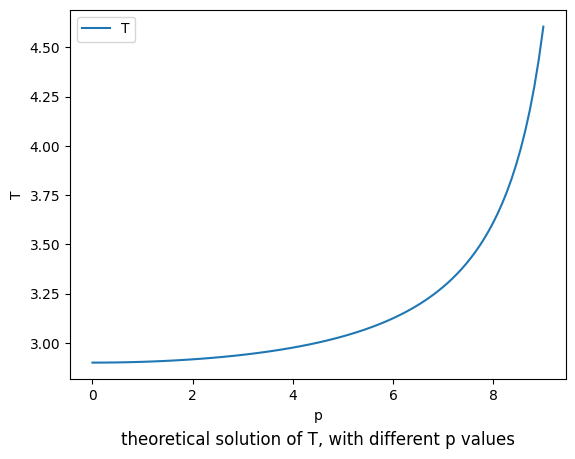
\includegraphics[width=12cm]{theory_T_diff_p.png}}
	\caption{The theoretical optimal T values against p values in the uncertainty set, from the formulation \ref{eq_Theory_T}}
	\label{theory_T_diff_p}
\end{figure}

We can also verify the accuracy of the theoretical solution through numerical means. To start, we showcase the behavior of the theoretical solution for $T$ as $p$ varies over the entire uncertainty set $\mathbb{P}=[0,9]$, as displayed in Figure \ref{theory_T_diff_p}. Next, we remove the uncertainty by presenting the solution to the original problem \ref{rc} for several selected $p_i$ values, where $p_i \in [p_0, p_1, ..., p_n] \subset \mathbb{P} = [0,9]$. To illustrate, we have chosen $p=0$, $p=5$, and $p=9$ as examples. Figures \ref{theory_ut_3p} demonstrate the theoretical $T$ values and corresponding $u(t)$ values for these three $p$ values.


\begin{figure}[h]
	\centerline{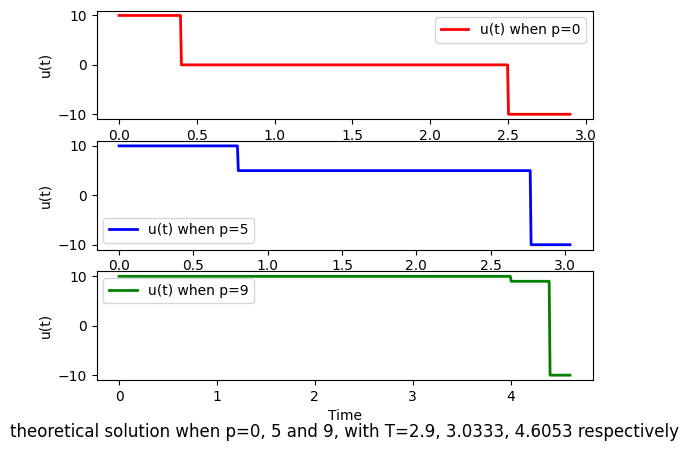
\includegraphics[width=12cm]{theory_ut_3p.png}}
	\caption{The theoretical u(t) values when p=0, p=5 and p=9, from the formulation \ref{eq_Theory_u}}
	\label{theory_ut_3p}
\end{figure}

When $p$ is fixed, the OCP under uncertainty reduces to a normal OCP problem, which can be solved directly with the numerical methods discussed in Chapter \ref{Chapter2}, without the need for bilevel optimization. We discretize $[0,1]$ into $500$ subintervals $\mathbb{I}j = [\tau{j-1}, \tau_j]$, with the discretization points as $0 = t_0 < t_1 < \dots < t_m = t_f = 1$. Using an error tolerance level of $1e-6$ and the Runge-Kutta RK4 method, the results obtained from solving the normal OCP with $p=0$, $p=5$ and $p=9$ are shown in Figure \ref{fig1_org_u10_p0}, Figure \ref{fig1_org_u10_p5} and Figure \ref{fig1_org_u10_p9} respectively.

These three figures \ref{fig1_org_u10_p0}, \ref{fig1_org_u10_p5}, and \ref{fig1_org_u10_p9} demonstrate that the results obtained from $p=0$, $p=5$, and $p=9$ are consistent with the theoretical results presented in formulations \ref{eq_Theory_T} and \ref{eq_Theory_u}, as shown in Figure \ref{theory_T_diff_p} and Figure \ref{theory_ut_3p}. This confirms two points: first, the theoretical results are correct, and second, the numerical methods we have selected can solve the rocket car problem for a fixed $p$ value. These methods can, therefore, be applied to solve general OCPs.


\begin{figure}[H]
	\centerline{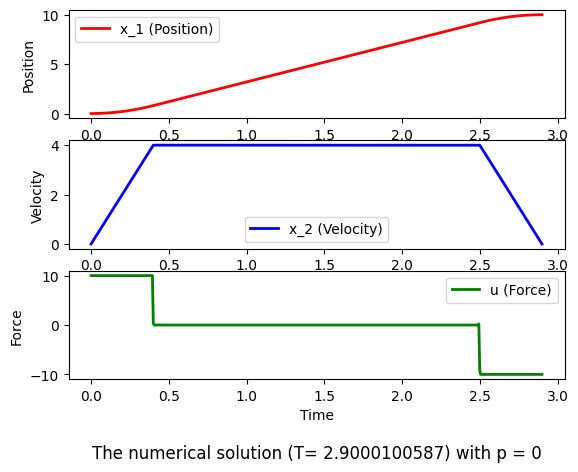
\includegraphics[width=10cm]{original_u10_p0.png}}
	\caption{Orginal rocket car problem \ref{rc} solution when p=0}
	\label{fig1_org_u10_p0}
\end{figure}

\begin{figure}[H]
	\centerline{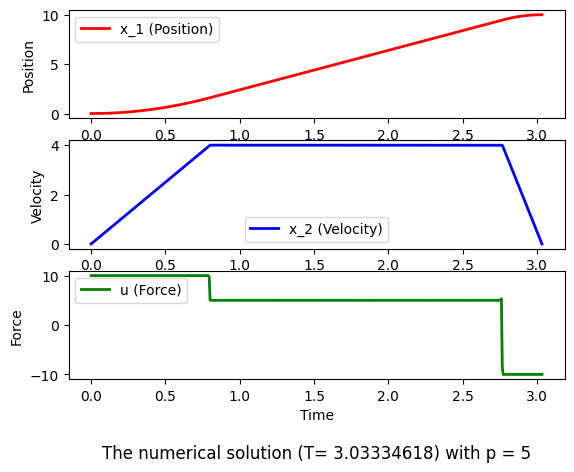
\includegraphics[width=10cm]{original_u10_p5.png}}
	\caption{Orginal rocket car problem \ref{rc} solution when p=5}
	\label{fig1_org_u10_p5}
\end{figure}

\begin{figure}[H]
	\centerline{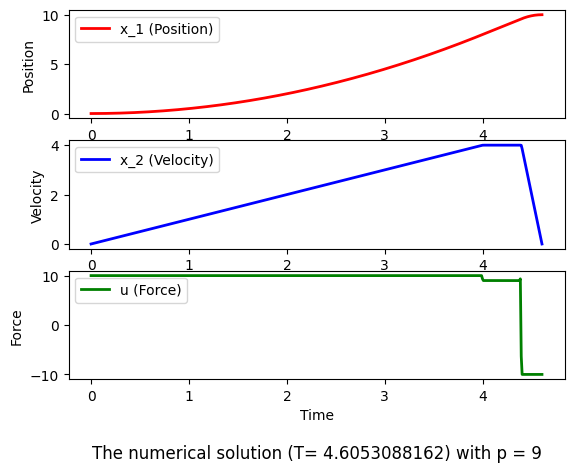
\includegraphics[width=10cm]{original_u10_p9.png}}
	\caption{Orginal rocket car problem \ref{rc} solution when p=9}
	\label{fig1_org_u10_p9}
\end{figure}

The rocket car case provides a simple problem for which we can obtain the theoretical solution to the original problem. However, in many real-life scenarios, finding a direct solution to the original problem is challenging and may not be feasible due to uncertainty in the parameter $p$. To address this challenge, the paper \cite{MatSch22} proposes both classical and training approaches, which yield conservative solutions to the original problem. A conservative solution is desirable as it reduces risk and improves robustness.

After discretizing the uncertainty set, the problem becomes a normal optimal control problem that can be solved using the multiple shooting and quasi-Newton (in the SQP framework) method. We utilize the open-source packages Casadi\footnote{Refer to https://web.casadi.org for more details} and Gekko\footnote{Refer to https://gekko.readthedocs.io/en/latest/ for more details} for solving the problem. These packages allow users to choose different nonlinear programming solvers and underlying numerical methods. For our problem, we have used the multiple shooting and sequential quadratic programming method with the underlying numerical integration using the Runge-Kutta RK4 method. We discretize $t \in [0,1]$ into $500$ subintervals $\mathbb{I}_j = [\tau_{j}, \tau_{j+1}]$, where $0 = t_0 < t_1 < ... < t_m = t_f =1$, and set the error tolerance level to $1e-6$. The numerical results from the classical and training approaches will be presented in the next two sections.


\section{Apply classical (minmax) approach}
In Section \ref{Sec:CA}, we explained the classical approach, and in this section, we present the numerical results of applying the classical approach to the chosen rocket car case.

First, we discretize the entire uncertainty set $\mathbb{P}$ into multiple points in increasing order $[p_0, p_1, \dots, p_n] \subset \mathbb{P}$ so that $p_i, i=0, 1, \dots, n$ can approximate the whole set $\mathbb{P}$ when $n$ is large enough. Here $p_0=p_l$ and $p_n=p_u$, with $[p_l, p_u]=[0,9]$, as shown in equation \ref{uncertainP}. We solve the $minmax$ problem in the following form
\begin{subequations}
	\begin{align}
		\underset{\epsilon, u(\cdot), x(\cdot)}{min}  \ \   &  \underset{p_i \in \mathbb{P}}{max}  \  \epsilon \\ 
		s.t.  &  \ \ T_i  \leq \epsilon \\
		&  \ \ x = (x_1, x_2),   \label{ca_rc_x} \\ 
		& \ \  \dot{x} = T_i  \begin{pmatrix}  x_2(t) \\ u(t)-p_i   \end{pmatrix}, &  \ \forall \   p_i, \  t \in [0,1],  \label{ca_rc_partial} \\
		& \ \ x(0) = 0, \label{ca_rc_t0}\\
		& \ \ x_1(1) \geq 10  \   \label{ca_rc_x1_t1} \\
		& \ \ x_2(t) \leq 4,  \    t \in [0,1] \label{ca_rc_x2_tc} \\
		& \ \ x_2(1) \leq 0,   \label{ca_rc_x2_t1}  \\
		& \ \ T \geq 0, \\
		& \ \ u(t) \in [-10, 10],  \ t \in [0,1]. 
	\end{align}
	\label{ca_rc}
\end{subequations}
for all $p_i$ where $p_i \in [p_0, p_1, ..., p_n] \subset \mathbb{P}$. Both $u(\cdot)$ and $x(\cdot)$ are functions of $t$ and need to be discretized in the time horizon (i.e., $500$ subintervals). In this classical approach, the driver has no prior knowledge about the value of the parameter $p$ and receives no feedback during the process, so they must set up the driving strategy in advance. Consequently, the realization of the trajectory of $u(\cdot)$ and $x(\cdot)$ for each $p_i$ may not be an optimal solution compared to the case when knowing the value of $p_i$ in advance.

\begin{figure}[H]
	\centerline{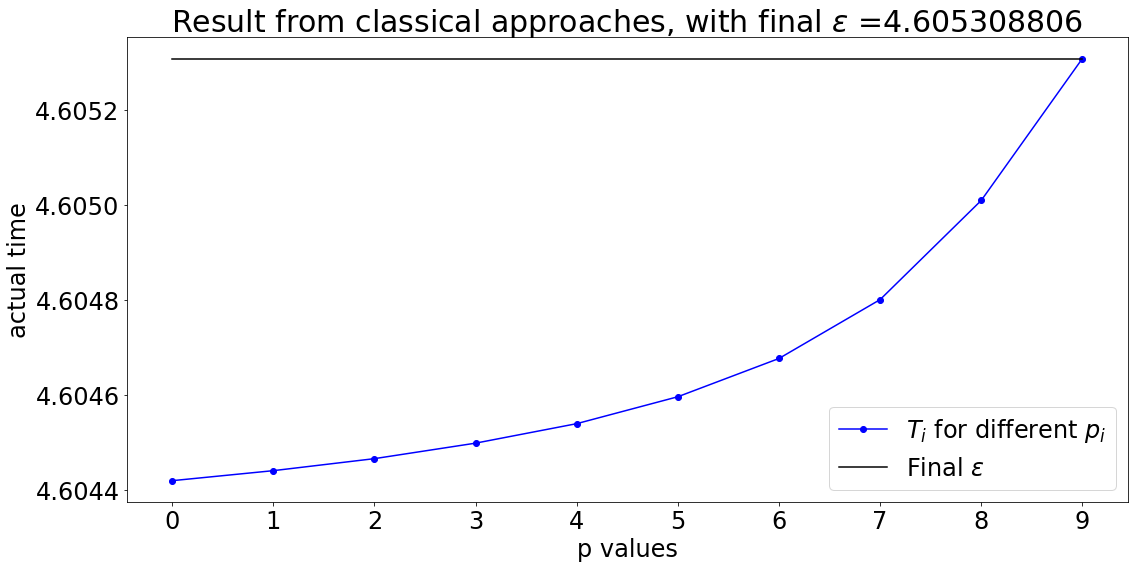
\includegraphics[width=13cm]{ca_result.png}}
	\caption{Final $\epsilon$ and $T_i$ for different $p_i$ values}
	\label{fig_ca_result}
\end{figure}


For each $p_i$ in the set $[p_0, p_1, ..., p_n] \subset \mathbb{P}$, we obtain a corresponding value of $T_i$, which we maximize over $T_i, i =0, 1, ..., n$. We aim to minimize $\epsilon$ ($\epsilon = \underset{i}{max} \ T_i$). Ultimately, we obtain a worst-case $\epsilon$ value over all $T_i$ for $i=0,1,...,n$, and for each $i$, we get a trajectory $(p_i, x(t;p_i), (t;p_i))$.

In our implementation, we set $n=40$, covering the entire uncertainty set $\mathbb{P}=[0,9]$. However, for the sake of readability, we only show results for $p_i=0, 1, 2, 3, 4, 5, 6, 7, 8, 9$. Figure \ref{fig_ca_result} displays the final time $\epsilon$ and $T_i$, where $\epsilon = \max_i T_i$ and the maximum value is achieved when $p_i=9$, with $\epsilon$ reaching a value of $4.6053$. Differences in $T_i$ mainly arise due to numerical errors, with our implementation using 500 subintervals and a numerical error tolerance of $1e-6$. Increasing the number of subintervals and decreasing the tolerance level should result in $T_i$ values for $p_i \neq 9$ converging to those of $p_i=9$.

The trajectories $(p_i, x(t;p_i), (t;p_i))$ for $p_i=0, 1, 2, 3, 4, 5, 6, 7, 8, 9$ are depicted in Figures \ref{fig_ca_ut_pis}, \ref{fig_ca_st_pis}, and \ref{fig_ca_vt_pis}. In all three figures, the standardized time $t \in [0,1]$ is used as the x-axis. Figure \ref{fig_ca_ut_pis} shows the $u(t)$ acceleration/deceleration force for each $p_i$ value, while Figure \ref{fig_ca_st_pis} displays the position $x_1(t)$ and Figure \ref{fig_ca_vt_pis} displays the velocity $x_2(t)$ for each $p_i$.



\begin{figure}[H]
	\centerline{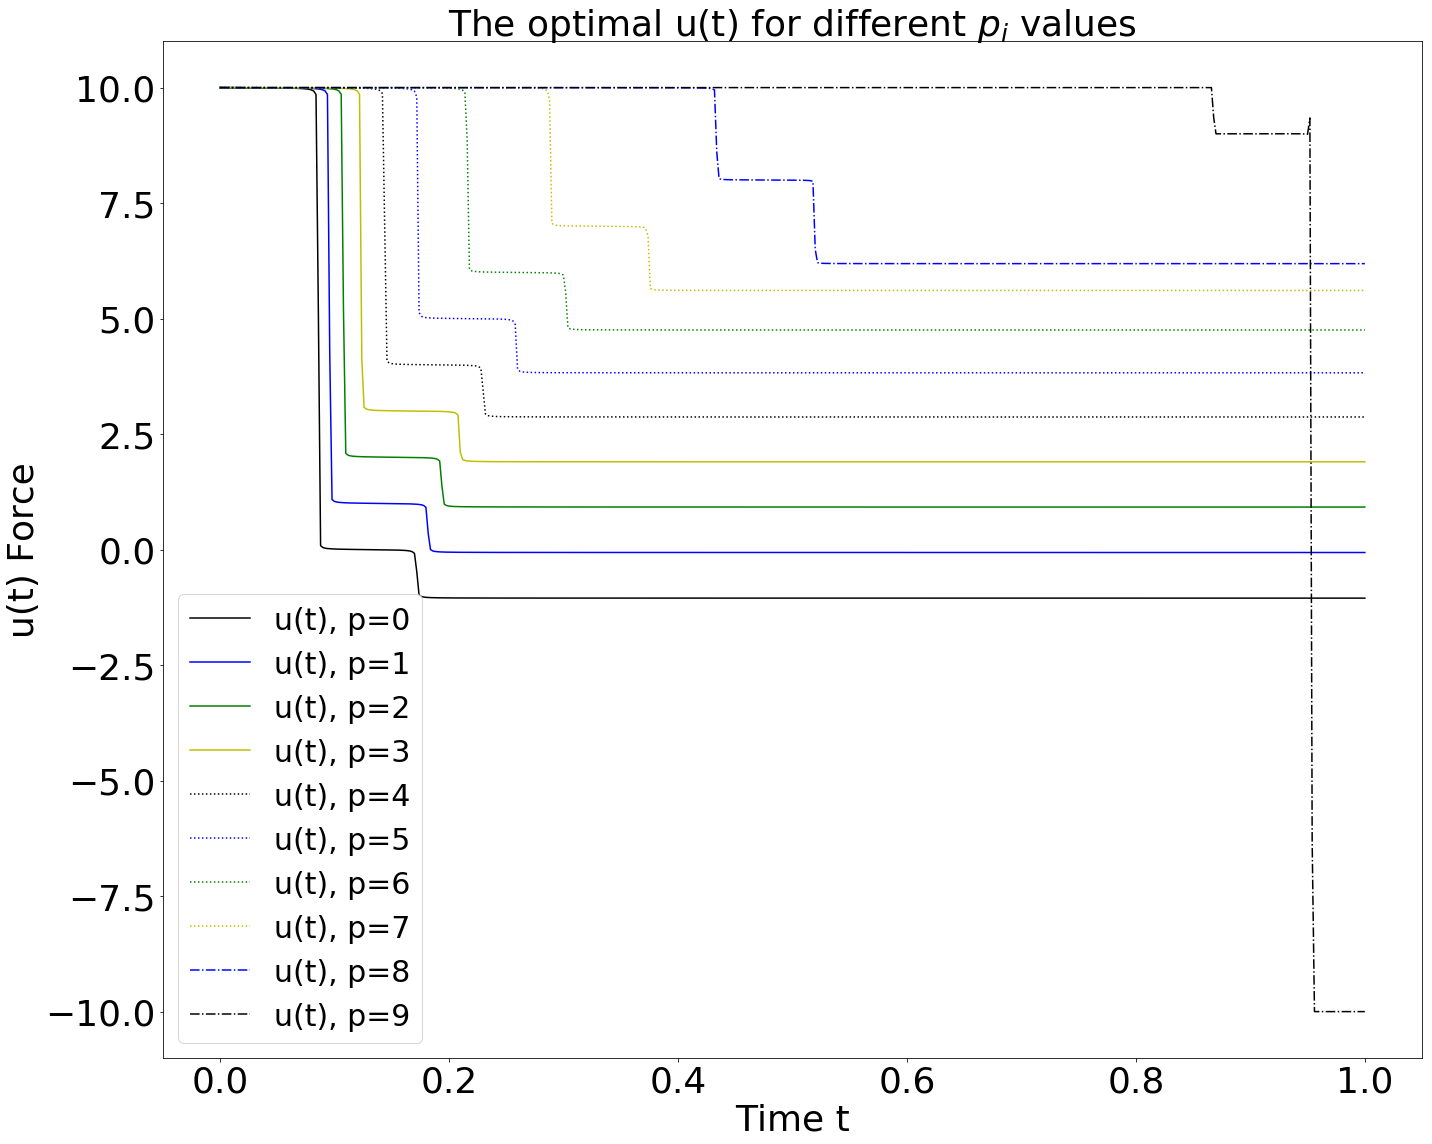
\includegraphics[width=13cm]{ca_ut_pis.png}}
	\caption{u(t) Force for different $p_i$ values}
	\label{fig_ca_ut_pis}
\end{figure}

\begin{figure}[H]
	\centerline{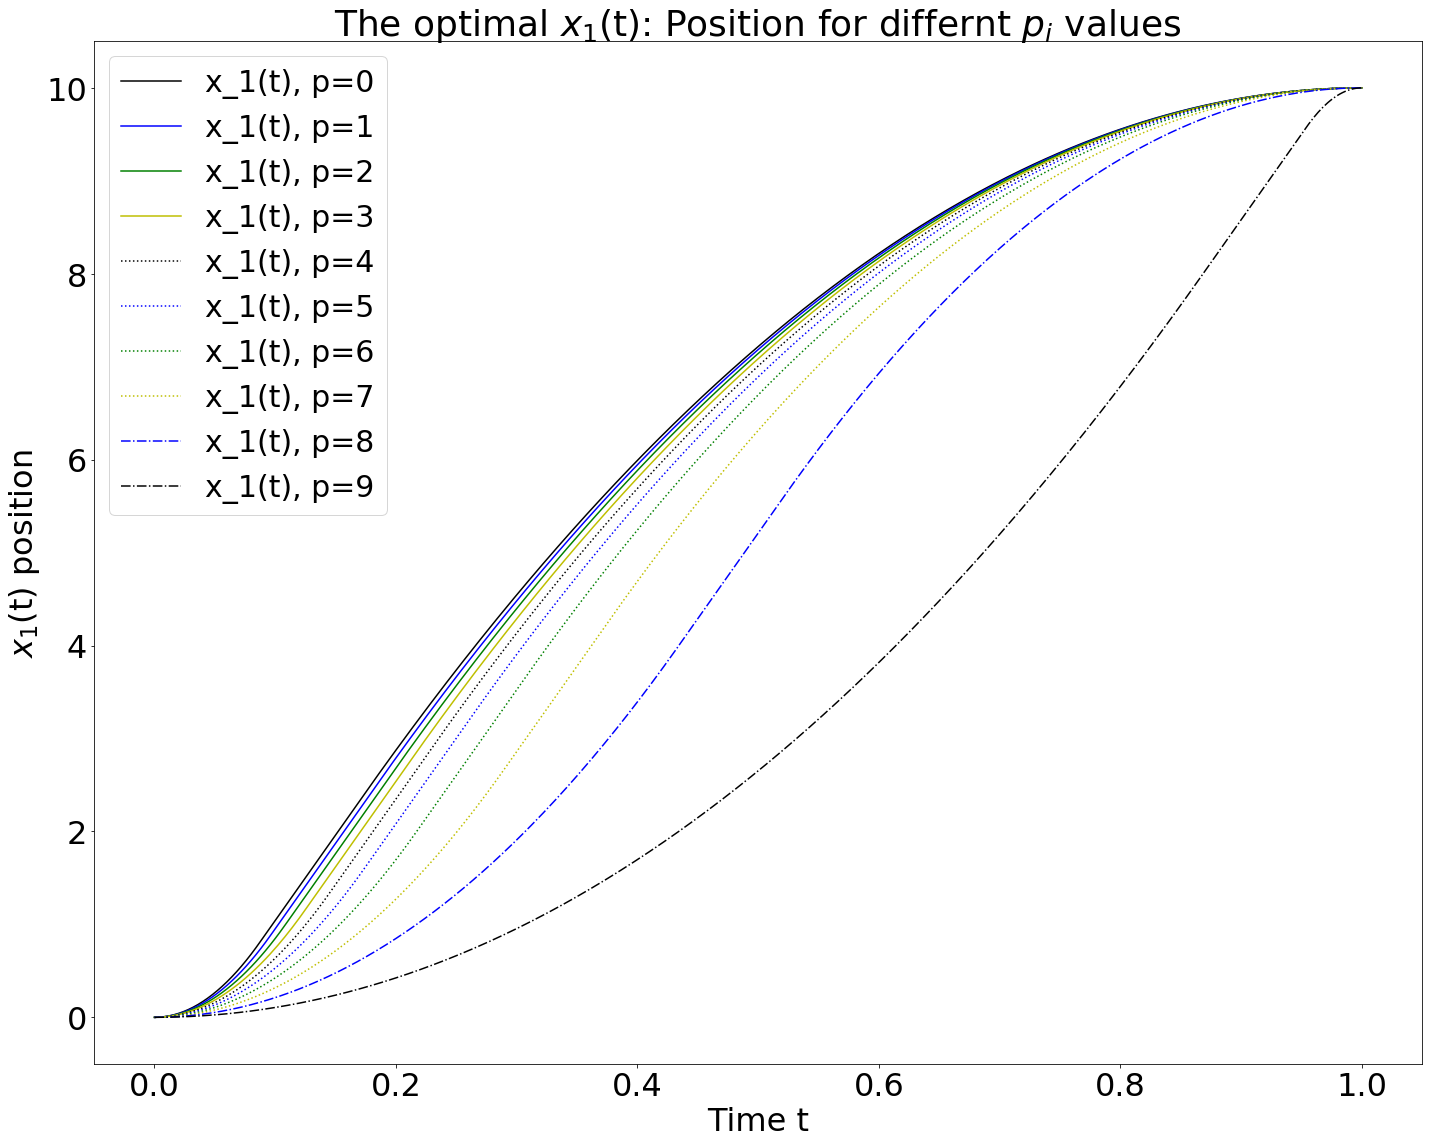
\includegraphics[width=13cm]{ca_st_pis.png}}
	\caption{$x_1(t)$ Position for different $p_i$ values}
	\label{fig_ca_st_pis}
\end{figure}

\begin{figure}[H]
	\centerline{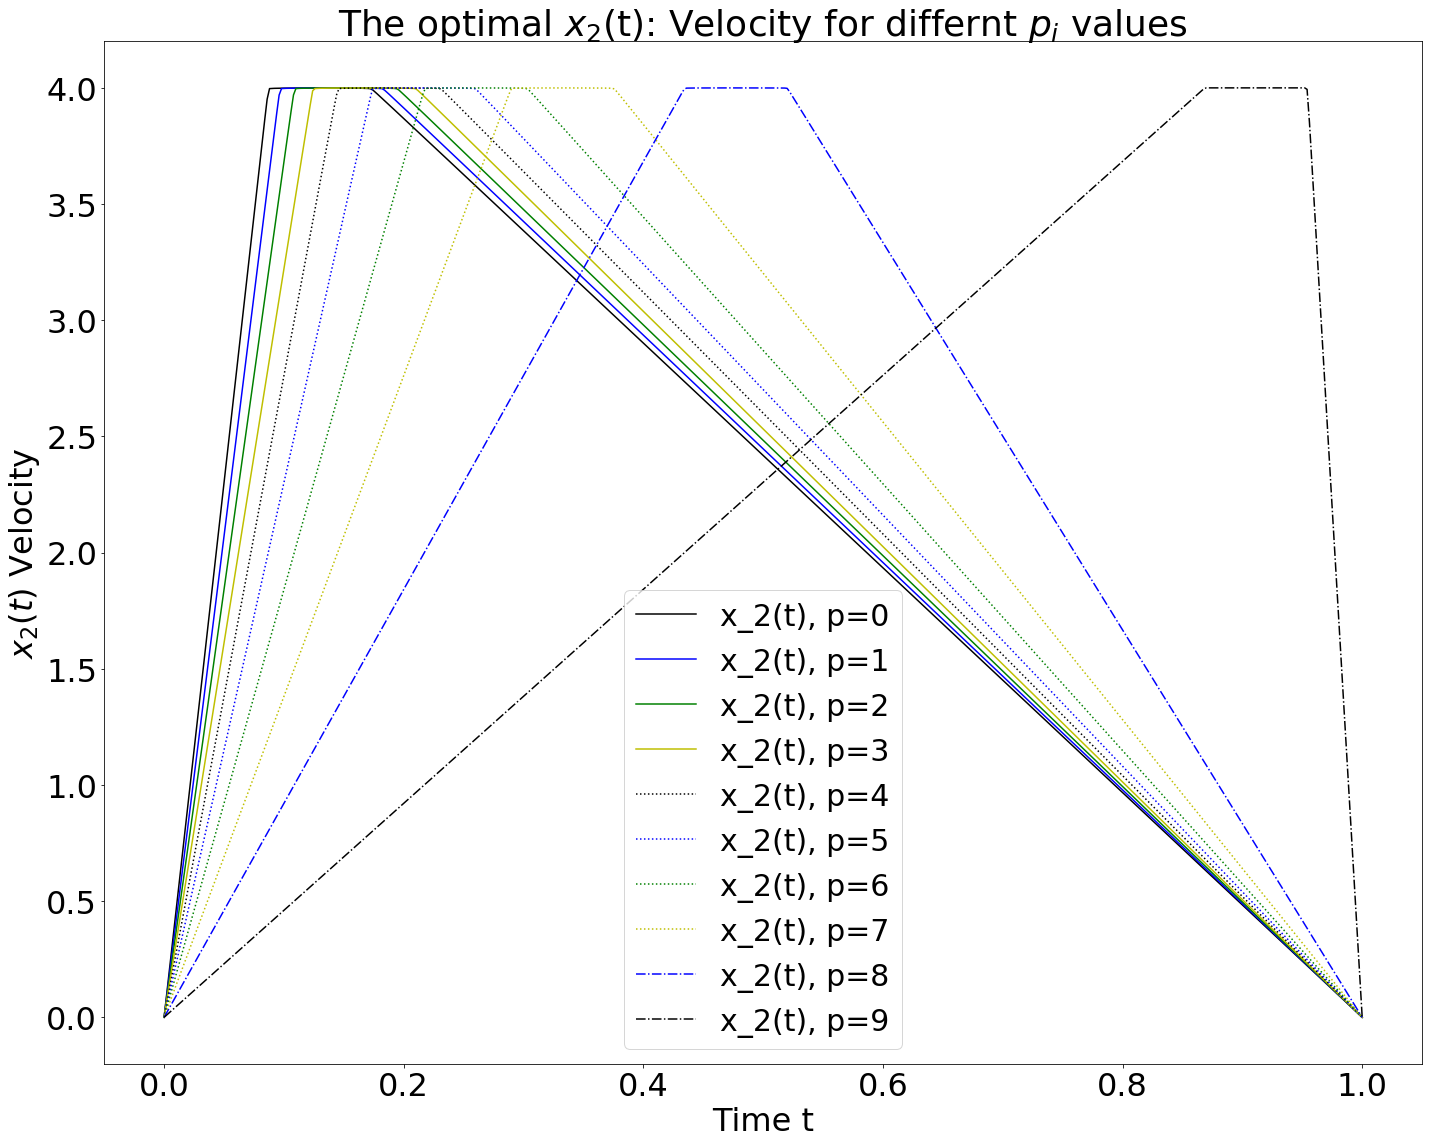
\includegraphics[width=13cm]{ca_vt_pis.png}}
	\caption{$x_2(t)$: Velocity for different $p_i$ values}
	\label{fig_ca_vt_pis}
\end{figure}


We have previously discussed that trajectories for different values of $p_i$ obtained using the classical approach may not be optimal compared to the solutions obtained by directly solving the OCP \ref{rc} with known values of $p_i$. In this section, we compare the trajectories obtained from the classical approach with the results of solving OCP \ref{rc} directly with $p_i=0$, $p_i=5$, and $p_i=9$. Figures \ref{fig1_org_u10_p0}, \ref{fig1_org_u10_p5}, and \ref{fig1_org_u10_p9} already show the results of solving OCP \ref{rc} directly with $p_i=0$, $p_i=5$, and $p_i=9$.

In Figures \ref{fig_ca_compare_p0}, \ref{fig_ca_compare_p5}, and \ref{fig_ca_compare_p9}, we present a comparison between the solutions obtained using the classical approach and the solutions obtained by directly solving OCP \ref{rc} for $p_i=0$, $p_i=5$, and $p_i=9$. From Figures \ref{fig_ca_compare_p0} and \ref{fig_ca_compare_p5}, it is clear that the classical approach leads to more conservative solutions than directly solving OCP \ref{rc} for $p_i=0$ and $p_i=5$, respectively. However, when $p_i=9$, as shown in Figure \ref{fig_ca_compare_p9}, the classical approach yields the worst-case scenario, and the corresponding $\epsilon=4.6053$ is equal to the result of directly solving OCP \ref{rc} with $p_i=9$. For any other value of $p_i \neq 9$, we can always find a feasible solution with a corresponding $T_i$, which will be less than or equal to $4.6053$.





\begin{figure}[H]
	\centerline{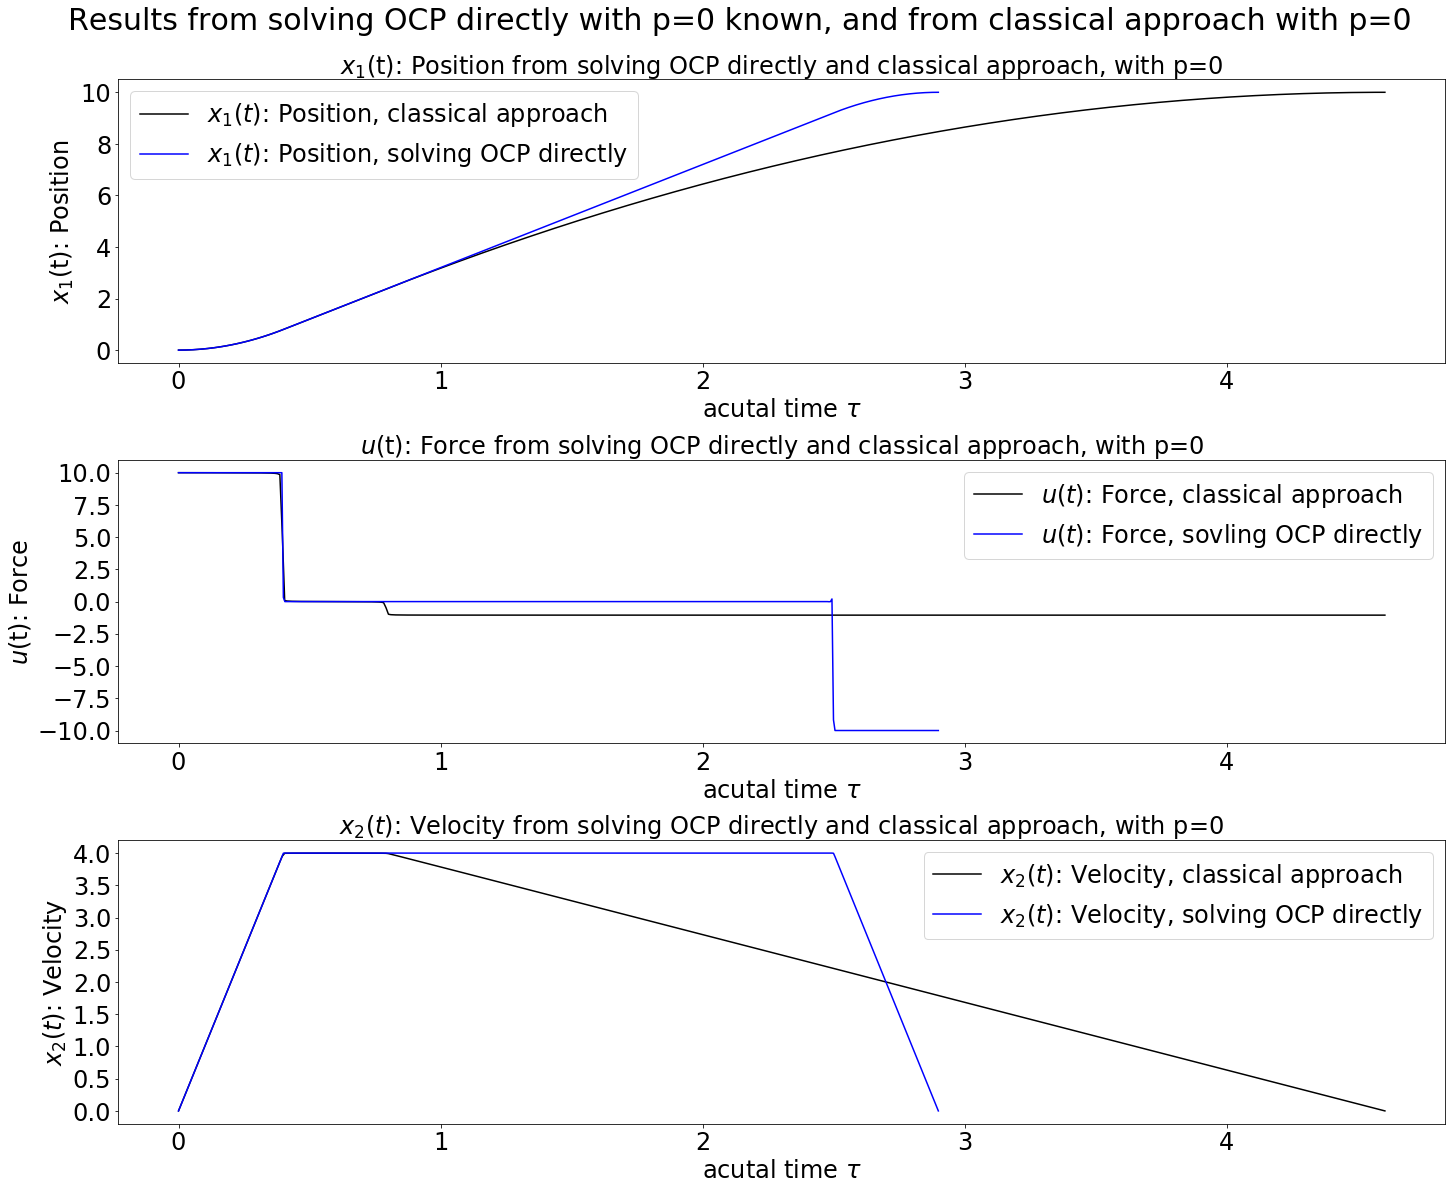
\includegraphics[width=12.5cm]{ca_compare_p0.png}}
	\caption{Compare the results from solving OCP \ref{rc} with $p=0$ and the result of applying the classical approach to problem \ref{ca_rc} with $p=0$}
	\label{fig_ca_compare_p0}
\end{figure}

\begin{figure}[H]
	\centerline{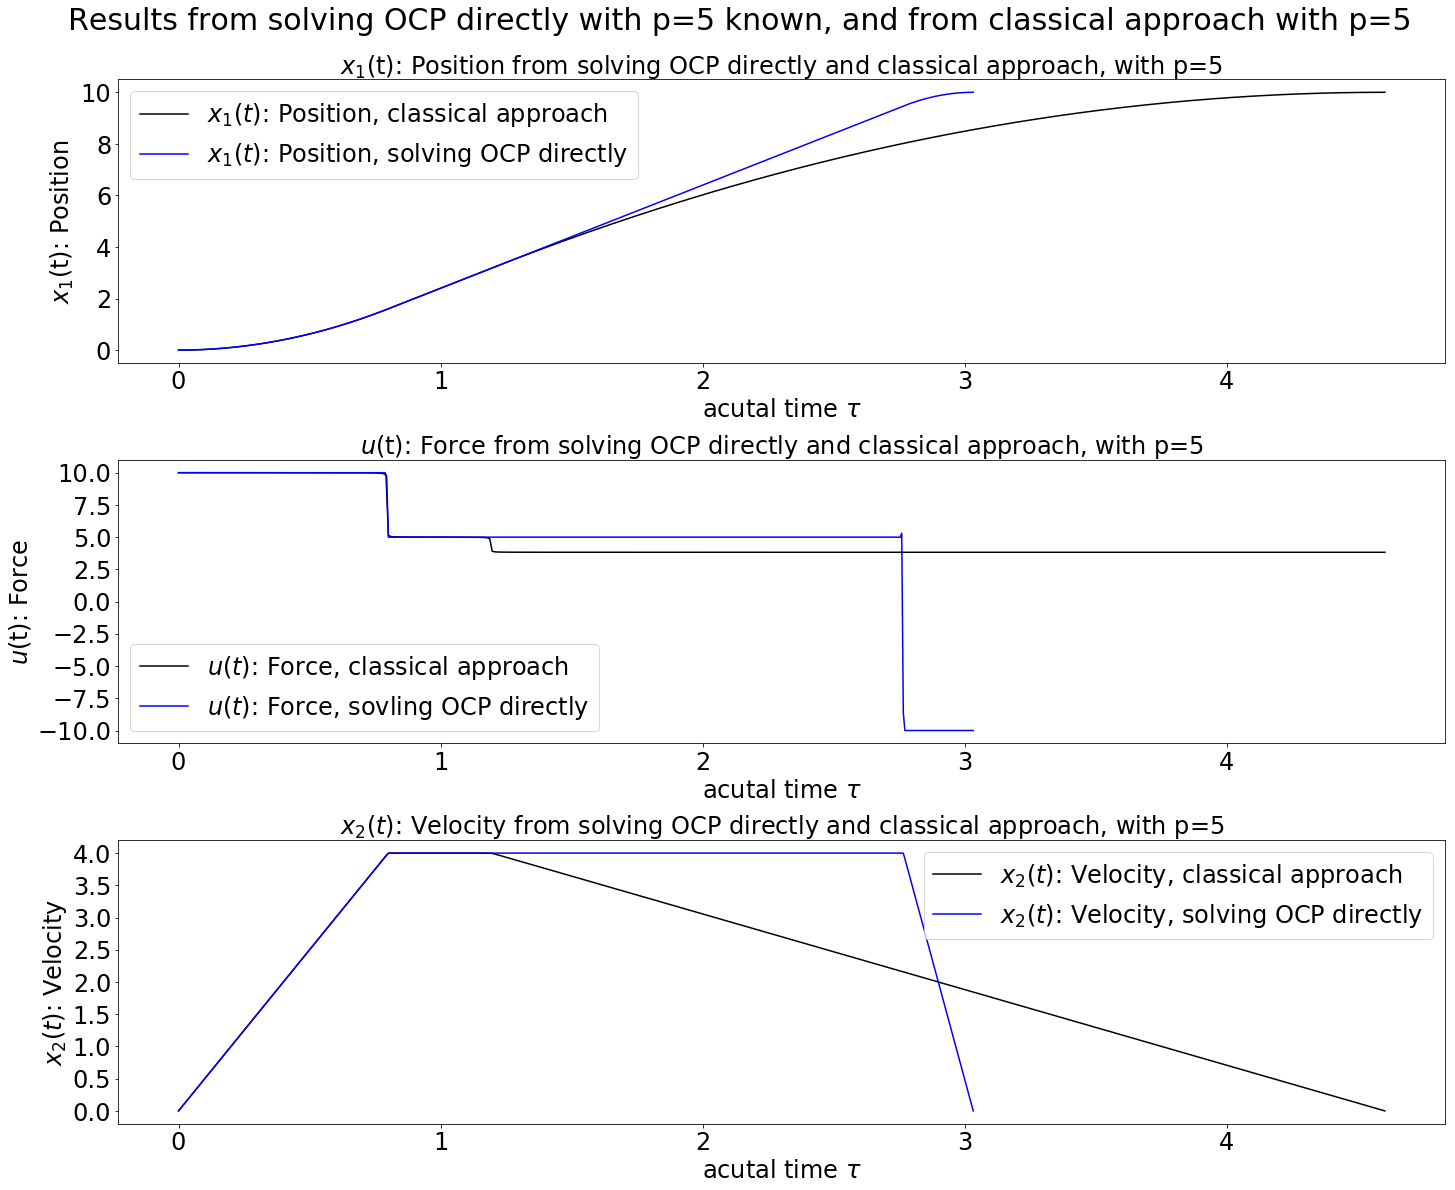
\includegraphics[width=12.5cm]{ca_compare_p5.png}}
	\caption{Compare the results from solving OCP \ref{rc} with $p=5$ and the result of applying the classical approach to problem \ref{ca_rc} with $p=5$}
	\label{fig_ca_compare_p5}
\end{figure}

\begin{figure}[H]
	\centerline{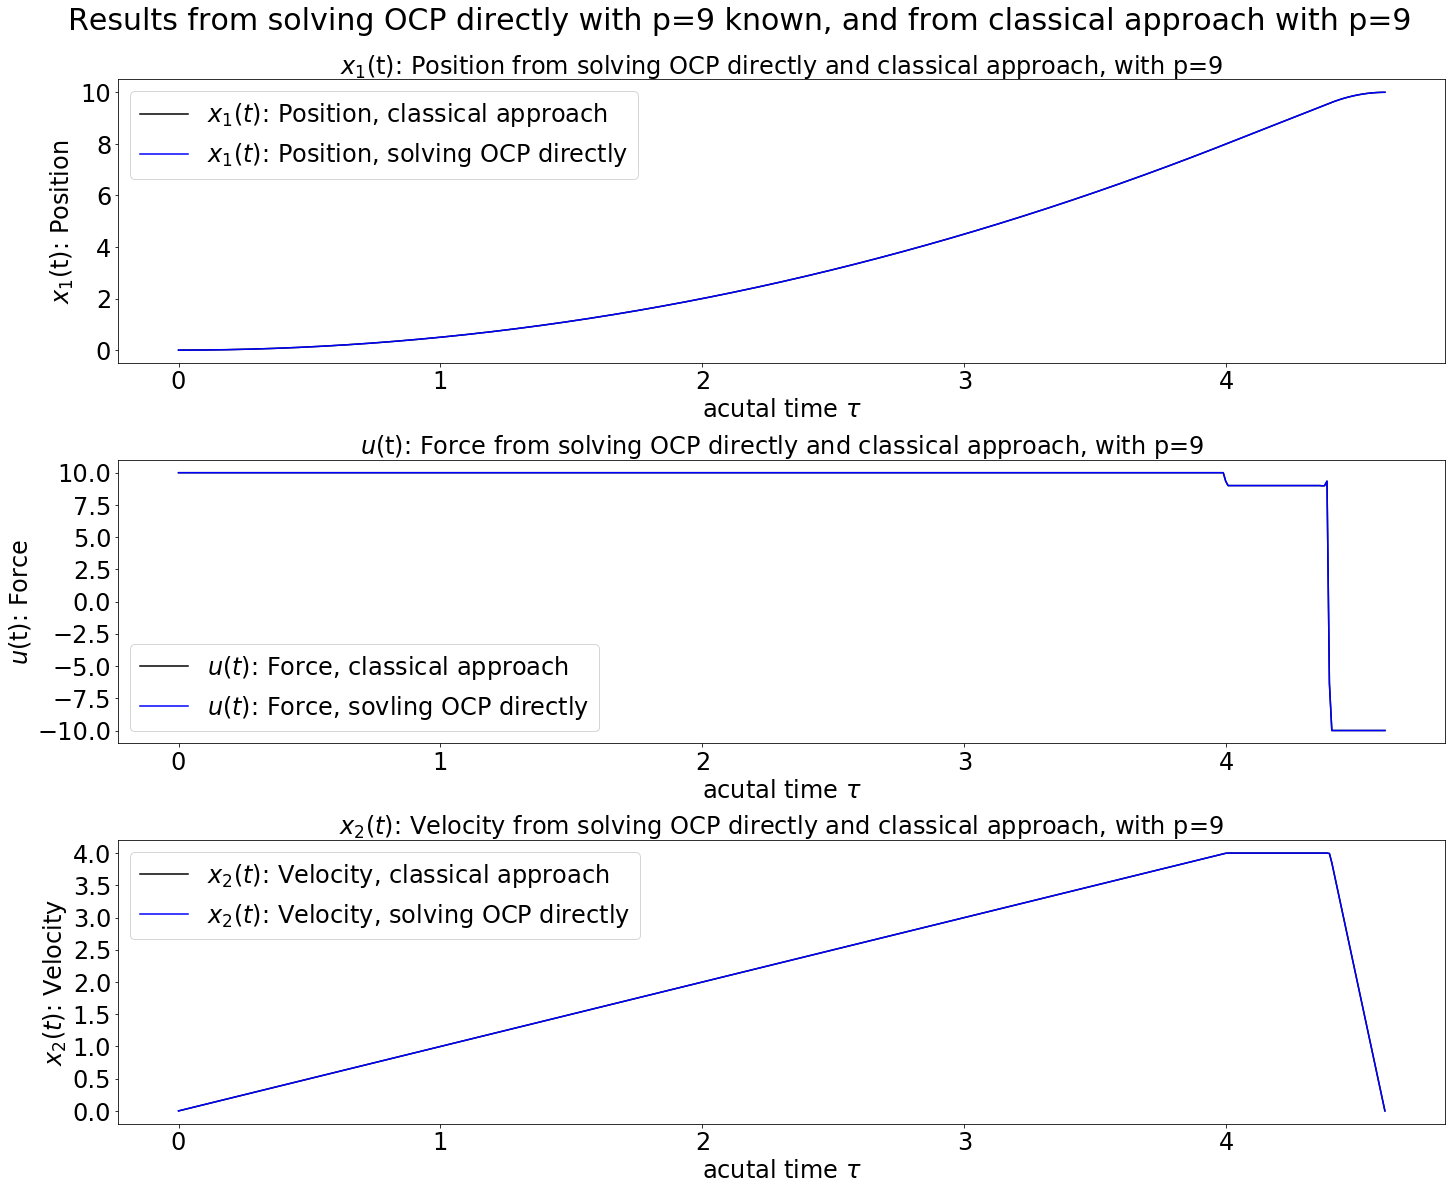
\includegraphics[width=12.5cm]{ca_compare_p9_old.png}}
	\caption{Compare the results from solving OCP \ref{rc} with $p=9$ and the result of applying the classical approach to problem \ref{ca_rc} with $p=9$}
	\label{fig_ca_compare_p9}
\end{figure}




 




\section{Apply training (maxmin) approach}
In contrast to the classical approach, the training approach assumes that the driver of the rocket car can perform optimally for any value of $p$, as a result of prior training. To discretize the uncertainty set $\mathbb{P}$, we use the same method as in the classical approach by selecting discrete points $p_0, p_1, ..., p_n$ that cover the entire uncertainty set $\mathbb{P}$. For each $p_i$ in the interval $[p_0, p_1, ..., p_n] \subset \mathbb{P}$, we solve the corresponding problem.
%Contrast to the classical approach, in the training approach it is assumed that the driver of the rocket car is able to perform optimally for every $p$ because of a preceding training period. We discretize the uncertainty set $\mathbb{P}$ the same as in the classical approach, i.e. we take the discretized points $p_0, p_1, ..., p_n$ which cover the whole uncertainty set $\mathbb{P}$.  For each $ p_i  \in [p_0, p_1, ..., p_n] \subset \mathbb{P}$, we solve the problem 
\begin{subequations}
	\begin{align}
		 \underset{p_i \in \mathbb{P}}{max}  \ \underset{T, u(\cdot), x(\cdot)}{min}  \ \   &   T  \\ 
		s.t.  & \ \ x = (x_1, x_2),   \label{ta_rc_x} \\ 
		& \ \  \dot{x} = T  \begin{pmatrix}  x_2(t) \\ u(t)-p_i   \end{pmatrix}, & \ t \in [0,1],  \label{ta_rc_partial} \\
		& \ \ x(0) = 0, \label{ta_rc_t0}\\
		& \ \ x_1(1) \geq 10, \label{ta_rc_x1_t1} \\
		& \ \ x_2(t) \leq 4, & t \in [0,1], \label{ta_rc_x2_tc} \\
		& \ \ x_2(1) \leq 0, \label{ta_rc_x2_t1}  \\
		& \ \ T \geq 0, \\
		& \ \ u(t) \in [-10, 10], & t \in [0,1]. 
	\end{align}
	\label{TA_rc}
\end{subequations}

\begin{figure}[H]
	\centerline{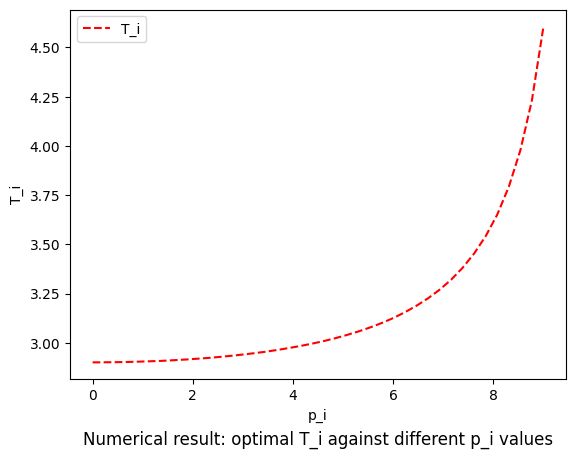
\includegraphics[width=10cm]{numerical_T_p.png}}
	\caption{Numerical result: different $T_i$ values against different $p_i$ values, with $p_i=9$ and  $T_i=4.6053$ the worst case}
	\label{fig_ta_numerical_T_p}
\end{figure}

After setting a value for $p_i$, we can solve a normal optimal control problem (OCP). Each $p_i$ value corresponds to one optimal $T_i$ value. Our goal is to find the worst-case scenario among all the optimal $T_i$ values, i.e., the largest among them. Similar to the discretization of the uncertainty set in the classical approach, here we also take $n=40$, i.e. in total $40$ $p_i$ points ranging the whole uncertainty set $\mathbb{P}=[0,9]$.  The resulting $T_i$ values for each $p_i$ are shown in Figure \ref{fig_ta_numerical_T_p}. This figure is almost identical to Figure \ref{theory_T_diff_p}, indicating that our numerical results with different $p$ values are consistent with the theoretical results. The worst-case scenario occurs when $p_i$ takes its maximum value of $9$, and in this case, $T_i=4.6053$. We have already shown the solution to the original problem for $p_i=9$ in Figure \ref{fig1_org_u10_p9}. Therefore, the worst-case scenario has the same solution as shown in Figure \ref{fig1_org_u10_p9} with $T=4.6053$, which we repeat in Figure \ref{fig1_ta_final}.

\begin{figure}[h]
	\centerline{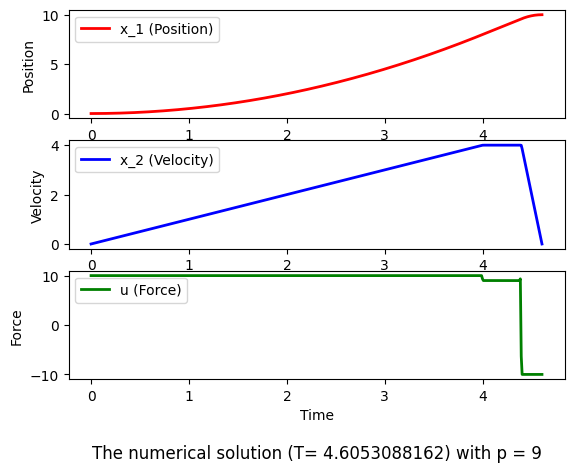
\includegraphics[width=10cm]{original_u10_p9.png}}
	\caption{Training approach to problem \ref{TA_rc}, final result, worst case happens when $p=9$}
	\label{fig1_ta_final}
\end{figure}


\section{Analysis the numerical results}
\label{Sec_NR}

In addition to the numerical results discussed above, this section includes additional numerical analysis and a discussion of all the numerical results.

\subsection{Sensitivity with initial value}

In this section, we demonstrate the stability of our numerical implementation with respect to different initial values $u(t_0) \in [0,10]$. As previously explained, the rocket car should accelerate as fast as possible at the beginning, i.e., $u(t_0)$ should take the maximum allowable value of $10$ in order to obtain the optimal/smallest $T$. With different $u(t_0) \in [0,10]$, the control variables $u(t)$ will move towards $10$ during the acceleration stage, as shown in the first subplot of Figure \ref{fig1_initialUt}. We have used only $100$ subintervals for $[0,1]$ in this plot. As demonstrated in the second subplot of Figure \ref{fig1_initialUt}, when the initial value of $u(t_0)$ deviates from the ideal initial value $u(t_0)=10$, it takes the longest time $T$, compared to other initial values. As the number of subintervals increases, the $T$ associated with initial values other than $u(t_0)=10$ converges to $T^\star(u(t_0)=10)$. The results of this section confirm the background knowledge discussed in this paper and the theoretical solution.



 \begin{figure}[h]
	\centerline{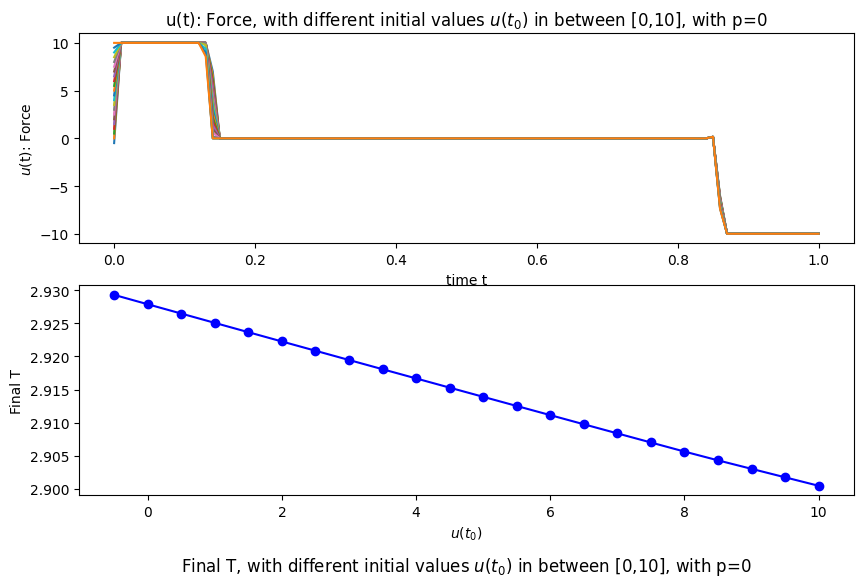
\includegraphics[width=12cm]{initial_value.png}}
	\caption{Results of solving OCP directly, with $p=0$ and different initial values $u(t_0)$ in the set [0,10]. }
	\label{fig1_initialUt}
\end{figure}\textbf{}



\subsection{Shared control $u(t)$ for classical approach}
\label{Sec_ShareUt}

In the classical approach, a feasible solution $u(:,p), x(:,p)$ can be found for each $p$ when solving the lower level part. However, if we force a unified $u(t)$ for all $p$ in the uncertainty set, we cannot find a feasible $u(t)$ that satisfies all $p$ values if the uncertainty set is too large. If we narrow down the uncertainty set, for example, by setting it to $\mathbb{P}=[0,1]$, we can still find a feasible solution with shared control states $u(t)$ for all the parameters within the uncertainty set, as shown in Figure \ref{fig1_ca_unifiedUt}. The trajectories for both $x(t)$ and the shared $u(t)$ at the boundary parameters $p=0$ and $p=1$ satisfy the constraints, as shown in the subplots for "$x_1:$ Position" and "$x_2:$ Velocity". However, if we increase the uncertainty set, we fail to find a shared $u(t)$ that leads to feasible solutions for all $p$ in $\mathbb{P}=[0,9]$. This is consistent with the theoretical analysis discussed in the next section, Section \ref{Comparison}, which shows that the classical approach will not yield a better solution than the training approach.



 \begin{figure}[H]
  	\centerline{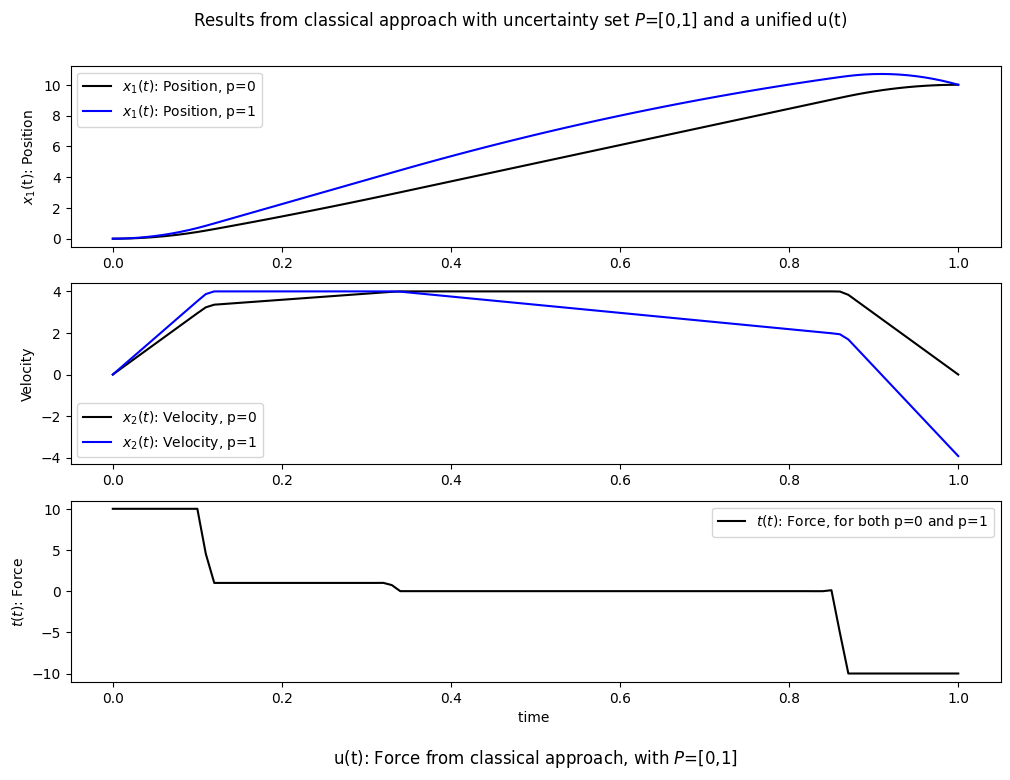
\includegraphics[width=10cm]{aunified_ut.png}}
  	\caption{Results from classical approach with a unified $u(t)$ with uncertainty set  $ \mathbb{P}=[0,1]$, with $T=2.9495636746$ when $p=0$, and $T=3.9240282505$ when $p=1$. }
  	\label{fig1_ca_unifiedUt}
  \end{figure}
  
  
\subsection{Comparison between classical approach and training approach]}
\label{Comparison}
In theory, the classical approach is expected to result in a solution that is inferior to the training approach. This is because in the training approach, the value of $p$ is known in advance, and the worst-case solution is obtained by maximizing over all $p \in \mathbb{P}$. However, in the classical approach, the value of $p$ is a priori unknown, and we must find solutions that yield parameter-dependent variables for all possible realizations of the uncertain parameters. Then, among these solutions, we need to find the optimal one. We won't go into the proof here, but we refer to \cite{MatSch22} for details. The conclusion of this theoretical result is shown directly in Theorem \ref{Theorem_compare}. In addition, we present an example to support this idea.



\begin{theorem} Let $\Omega_x \subset \mathbb{R}^{n_x}$ and $\Omega_p \subset \mathbb{R}^{n_p}$ be compact subsets and $f : \Omega_x *  \Omega_p \  \rightarrow \mathbb{R}$ a continuous function. Then we have
	\begin{equation}
	\underset{p \in \Omega_p}{max}\ \underset{x \in \Omega_x}{min}\ f (x,p) \leq \underset{x \in \Omega_x}{min}\ \ \underset{p \in \Omega_p}{max}\ f (x,p)
	\end{equation}
\label{Theorem_compare}
\end{theorem}

The optimal objective function value of the $max\ min$ problem in the training approach overestimates that of the $min\ max$ problem in the classical approach\footnote{The proof that $max\ min$  (training) approach over estimates that of $min \ max$ approach is given in paper \cite{MatSch22}}. Examples can be found easily where the gap between the two is greater than zero. For instance, suppose we take $\Omega_x=[-5,5]$ and $\Omega_p=[-1,1]$, and consider the function
$$
f : \Omega_x *  \Omega_p \  \rightarrow \mathbb{R}, \ (x,p) \rightarrow (x-p)^2 + p
$$
Then
$$	\underset{p \in \Omega_p}{max}\ \underset{x \in \Omega_x}{min}\ f (x,p) =1 \leq \frac{5}{4} = \underset{x \in \Omega_x}{min}\ \ \underset{p \in \Omega_p}{max}\ f (x,p)
$$

As shown above, both the classical and training approaches lead to an identical solution with a final time of $T=4.6053$, which is conservative with respect to the original OCP \ref{rc}. The time $T=4.6053$ is conservative regardless of how the uncertain parameter $p$ takes a value in the uncertainty set $\mathbb{P}$. We can always find a feasible solution that leads to a final time that is less than or equal to $T=4.6053$. Nevertheless, the classical and training approaches do not necessarily lead to an identical solution for a general OCP under uncertainty. In general, the classical approach should lead to a worse solution compared to the training approach. In our case, it just happens that both approaches lead to the same solution, and the worst-case scenario occurs when $p=9$ at the right boundary point.




\chapter{Conclusion}
\label{Chapter5}
In this paper, we have explained in theory how direct approaches can be used for solving optimal control problems. Within direct apporaches, mutiple shooting method is used to discretize the whole interval into subintervals, with the objective functions and constraints also discretized and applied piecewise for each subinterval. Matching condition is enforced at the boundary of each subinterval. With numerical methods such as Runge–Kutta method applied to the underlying dynamics system (i.e. differential equation) in each subinterval, the original OCP is turned into a piecewise nonlinear optimisation problem. We can, therefore, apply the KKT condition to incorporate the constraints and the objective function into a new Lagrange function, whose optimal solution can be found via its derivatives. Newton and quasi Newton is used and the Lagrange function optimal is found via the sequential quadrative approach. 

In real life, some OCPs may have uncertainty, in the form of unknown parameters $p$ in the uncertainty set  $\mathbb{P}$. Such problems is even harder to solve due to the uncertainty. In this case, we would like to have a conservative solution, which is worse than the optimal solution for a particular $p$ value regardless how the unknown parameter take values in the uncertainty set $\mathbb{P}$. There are two aproaches to reach the conservative solution, the classical approach and the training approach. 

For the numerical methods disscussed in this paper, their application is demostrated with a case study in state constrainted rocket car. When the unknown parameter $p$ takes a fixed value in the uncertainty set  $\mathbb{P}$, the OCP under uncertainty degenerates into a normal OCP problem and the solution can be obtained via mutiple shooting and quasi Netwon style method. The result have been shown in e.g.  Figure  \ref{fig1_org_u10_p0},  \ref{fig1_org_u10_p5} and \ref{fig1_org_u10_p9}. We have also perform a sensitivity analysis with respect to to the initial value, as shown in Figure \ref{fig1_initialUt}. The results confirms with our analysis that the numerical method we are using are stable and roubust.


We further continue the numerical implementation with classical approach and training approach, and both leads to a conservative solution. For our particular case, the conservative solutions from both approach are  the same. This is not contracdictory to our analysis that classical approach leads to a worse solution compared to traning approach. Actually, if we force the same control trajectory $u(t)$ for all the parameters $p \in \mathbb{P}$, no fesiable $u(t)$ can be found as explained in section \ref{Sec_ShareUt}, indicating the optimal $T$ is infinity. 

Therefore, we can conclude that our numerical results are consistent with our theorectical knowledge in the numerical methods discussed in this paper. These method can, therefore, be applied to more general optimal control problems and optimal control problems under uncertainty.  
   
\appendix
\chapter{Appendix  Runge–Kutta method}
  	\label{App1}
  	
  	The dynamic systems of the OCP in eqation \ref{P2_OPM} is defined in the subequation 
  	\ref{P2_sd}, which we show here independently
  	\begin{equation}
  		\dot{x} (t) = f(x(t), u(t)), \ \   t \in [t_0, t_f]
  		\label{eq_DS}
  	\end{equation}
  	If the initial value $x_0$ for \ref{eq_DS} is known, then equation \ref{eq_DS} becomes an initial value problem (IVP) and the solution can be found via numerical method. If analytical solutions exist for equation \ref{eq_DS}, then we can use the analytical solution directly. Nevertheless, for most real-life problems, the analytical solution either does not exist or is very difficult to find, and numerical method is the only practical way to find the solution. Given the initial value $x_0$, equation \ref{eq_DS} will have solution as 
  	%\begin{equation}
  	%	%	\begin{aligned}
  		%	x(t) -  x_0  &= \int_{t_0}^{t}  f(x(\tau), u(\tau)) d \tau,   \ \ t \in [t_0, t_f] \\ 
  		%	x(t) & = x_0  + \int_{t_0}^{t}  f(x(\tau), u(\tau)) d \tau,   \ \ t \in [t_0, t_f] 
  		%	\end{{aligned}
  	%	\label{eq_diffSolution}
  	%\end{equation}
  	\begin{equation}\label{eq_diffSolution}
  		\begin{aligned}
  			x(t) -  x_0  &= \int_{t_0}^{t}  f(x(\tau), u(\tau)) d \tau,   \ \ t \in [t_0, t_f] \\ 
  			x(t) & = x_0  + \int_{t_0}^{t}  f(x(\tau), u(\tau)) d \tau,   \ \ t \in [t_0, t_f] 
  		\end{aligned}
  	\end{equation}
  	
  	The integral in equation \ref{eq_diffSolution} can be approximated by numerical methods, and one simple approximation to the integral in equation \ref{eq_diffSolution} can be obtained via Euler method. The Euler method (also called forward Euler method) is a first-order numerical procedure for solving ordinary differential equations (ODEs) with a given initial value. Using a step size equal to 1, the approximation to equation \ref{eq_diffSolution} via Euler method is of the form
  	\begin{equation}
  		x(t)  = x_0  + \int_{t_0}^{t}  f(x(\tau), u(\tau)) d \tau \ \approx \   x_0  + t f(x(t_0), u(t_0))
  		\label{eq_Euler_approx}
  	\end{equation}
  	
  	Euler method is a first order and explicit method for approximating integrals, another widely used method is the trapezoidal rule, which is an implicit second-order method. The trapezoidal rule can approximate equation \ref{eq_diffSolution} as 
  	\begin{equation}
  		x(t)  = x_0  + \int_{t_0}^{t}  f(x(\tau), u(\tau)) d \tau \ \approx \   x_0  + \frac{t}{2}[f(x(t_0), u(t_0)) + f(x(t), u(t))]  
  		\label{eq_trapezoidal_approx}
  	\end{equation}
  	Notice, the soultion $x(t)$ becomes an input in the approximation in equation \ref{eq_trapezoidal_approx}, and that is why this method is classified as an implicit method. The trapezoidal rule belongs to the family of Runge–Kutta method, which is a family of implicit and explicit iterative methods, with various order of derivatives used. Among them, the Runge–Kutta  RK4 is the most widely used, which we describe in the following text. Let an initial value problem be specified as follows:
  	\begin{equation}\label{eqn:RK4_diff}
  		\dot{y} = f(t, y) , \ \  y(t_0) = y_0  
  	\end{equation}
  	
  	Here $y$ is an unknown function (scalar or vector) of time $t$, which we would like to approximate; we are told that $\dot{y} = \frac{dy}{dt}$, the rate at which $y$ changes, is a function of $t$ and of $y$ itself. At the initial time $t_0$ the corresponding $y$ value is $y_0$. The function $f$ and the initial conditions $t_0$, $y_0$ are given. Now we pick a step-size $h>0$ and define:
  	\begin{align}
  		y_{n+1} &= y_n + \frac{1}{6}\left(k_1 + 2k_2 + 2k_3 + k_4 \right)h,\\
  		t_{n+1} &= t_n + h
  	\end{align}
  	for $n = 0, 1, 2, 3, ...,$ using
  	\begin{align}
  		k_1 &= \ f(t_n, y_n), \\
  		k_2 &= \ f\!\left(t_n + \frac{h}{2}, y_n + h\frac{k_1}{2}\right), \\ 
  		k_3 &= \ f\!\left(t_n + \frac{h}{2}, y_n + h\frac{k_2}{2}\right), \\
  		k_4 &= \ f\!\left(t_n + h, y_n + hk_3\right).
  	\end{align}
  	
  	Here $y_{n+1}$ is the RK4 approximation of $y(t_{n+1})$, and the next value ($y_{n+1}$) is determined by the present value $(y_n)$ plus the weighted average of four increments, where each increment is the product of the size of the interval, $h$, and an estimated slope specified by function $f$ on the right-hand side of the differential equation.
  	\begin{itemize}
  		\item  $k_1$ is the slope at the beginning of the interval, using $y$  (Euler's method);
  		\item  $k_2$ is the slope at the midpoint of the interval, using $y$ and $k_1$;
  		\item  $k_3$ is again the slope at the midpoint, but now using $y$ and $k_2$;
  		\item $k_4$ is the slope at the end of the interval, using $y$ and $k_3$.
  	\end{itemize}
  	
  	
   % \chapter{Lists}
    %\listoffigures
    %\listoftables
    \newpage
    \bibliography{references}{}
     \newpage
    \citestyle{egu}
    \bibliographystyle{plainnat}
    \setlength{\parindent}{0em}

Erkl\"{a}rung:\par
\vspace{3\baselineskip}
Ich versichere, dass ich diese Arbeit selbstst\"{a}ndig verfasst habe und keine
anderen als die angegebenen Quellen und Hilfsmittel benutzt habe.\par
\vspace{5\baselineskip}
Heidelberg, den (Datum)\hspace{3cm}\dotfill
%
\vspace{8\baselineskip}

Declaration:\par
\vspace{3\baselineskip}
I hereby confirm that I wrote this work independently and did not use any sources other than those indicated.\par
\vspace{5\baselineskip}
Heidelberg, (Date)\hspace{3cm}\dotfill



  %\end{appendix}
 \newpage
\end{document}

